\documentclass[a4paper,12pt,twoside]{report}
\renewcommand{\baselinestretch}{1}

\usepackage{titlesec}

%all the other includes etc. are done in the thesis.sty file.
\usepackage{thesis}

%
% These commands need to be defined in order to produce a correct and personalized document
%
\newcommand{\shortdoctitle}{Improving Backtesting Environment}
\newcommand{\doctitle}{Aggressive Trade Prediction in the Foreign Exchange Market using XGBoost-Enhanced Neural Hawkes Process}
% \newcommand{\docsubtitle}{Under Extreme Class Imbalance, with Application in the FX Spot Market}
                       
\newcommand{\me}{Jiaxuan Zhu}
\newcommand{\stnumbr}{2838063}
\newcommand{\keywords}{Limit Order Book, Prediction, XGBoost, GRU, Hawkes Process
Foreign Exchange Market, Algorithmic Execution}

\newcommand{\customDate}{February 10, 2025}
\author{\me}

%
% PDF settings
%
\hypersetup
{
    pdfauthor={\me},
    pdftitle={\shortdoctitle},
    pdfsubject={\doctitle},
    pdfkeywords={\keywords}}




\makeatletter
\@removefromreset{page}{chapter}
\renewcommand{\thepage}{\arabic{page}}
\makeatother


\begin{document}
\renewcommand\bibname{References}
%use this include for PDF and distribution versions
%\pagenumbering{roman}
\begin{titlepage}
\begin{center}
% 
\includegraphics[height=2cm]{figures/Vu logo.png}\\
% 
\includegraphics[height=2cm]{figures/MN logo.png}\\
\begin{minipage}{0.5\linewidth}
    \centering
    
\includegraphics[height=2cm]{figures/Vu logo.png}
\end{minipage}%
\begin{minipage}{0.5\linewidth}
    \centering
    
\includegraphics[height=2cm]{figures/MN logo.png}
\end{minipage}

%\LARGE
%\VU Amsterdam \\
 \vspace*{10mm}
\large
Vrije Universiteit Amsterdam\\
School of Business and Economics\\
Master of Science in Econometrics\\


\vspace*{10cm}

\setlength{\TPHorizModule}{1mm}
\setlength{\TPVertModule}{\TPHorizModule}
% Set the Paragraph Indent to zero, so the first line is not Indented
% Back-up the current value so it can be put back at the end of the title page
\newlength{\backupparindent}
\setlength{\backupparindent}{\parindent}
\setlength{\parindent}{0mm}			
% Begins a textbox at 72 mm from the left of the edge of the paper and 89 mm from the top
% The width of the textbox is 95 mm (167 - 72 mm)
% The height of the box cannot be defined, so it is your task to keep the text not too long
\begin{textblock}{120}(50,109)
% \begin{textblock}{95}(62,109)

    \vspace*{1mm}
    \huge
    \textbf{\doctitle \\}
    \Large
    \vspace*{5mm}
    \textit{\docsubtitle}\\
    \vspace*{10mm}
    \Large
    \me\\
    Student number: \stnumbr\\
    \vspace*{5cm}
   
\end{textblock}

% \begin{textblock}{95}(62,209)
%     \vspace*{1mm}
%  \large
%     Supervisors: \firstCommitteeMember\\
%     \vspace*{5mm}
%     Policy Seminars and Policy Brief\\
%     \vspace*{5mm}
%     Location, \customDate\\
% \end{textblock}
% \vfill
\vspace{5cm}
\begin{tabular}{l l l}
    Thesis committee: & Dr. Ronald de Vlaming, & VU, supervisor \\
                      & E. Hazeveld, & MN, supervisor \\
\end{tabular}







% Put the Paragraph Indent back to its original value
\setlength{\parindent}{\backupparindent}
\end{center}

% Word count: xxxx

\end{titlepage} 

\normalsize
\begin{abstract}
\noindent 
% This thesis improves the high-frequency backtesting environment for Foreign Exchange markets by predicting realistic and dynamic aggressive trade patterns. The model is a novel XGBoost-Enhanced Neural Hawkes Process. It combines a neural Hawkes process with XGBoost to predict the occurance of aggressive trade based on the information in the limit order book.

% The main contribution is that the new framework enhances the standard Hawkes process by adding an XGBoost classifier and a neural kernel from GRU. The XGBoost first-filter solves the extreme trade and non-trade imbalance in the limit order book. The GRU neural kernel embeds the dynamic market features. The neural Hawkes process captures temporal dependency and clustering, and provides an interpretable outcome of when aggressive trades are likely to occur in the order flow. Unlike previous backtesting mechanism which uses static order filling rates, this approach gives more realistic and dynamic prediction of order filling status.

% Results show that the model captures the complex dynamics and patterns of aggressive trade perfectly. This can support better order filling methods for trading strategy backtesting.

% This work is relevant for those who want more realistic, dynamic and interpretable backtesting tools. Future work could extend the model to multi-asset settings or include more advanced market features.


This thesis improves backtesting environments for foreign exchange markets by predicting when aggressive trades will occur. The main problem is that when executing trades, aggressive traders often take passive orders out of the order book, but these events are difficult to predict. Aggressive trades are rare in the context of the overall order flow, cluster together in time, and depend on market conditions. Current backtesting systems use simple rules to decide when orders get filled, such as fixed probabilities based on bid-ask spreads. These methods do not capture the real dynamics of how trades happen in markets. When backtesting systems cannot predict these aggressive trades, the backtesting results underestimate filling rates and provide misleading performance results.

This study develops a novel framework with two stages to predict aggressive trades. First, an XGBoost filter addresses the extreme class imbalance problem. Second, a neural network captures embedded market features over time and passes the kernel to a Hawkes process, creating a neural Hawkes process. 

Results show that the model successfully captures the temporal dependencies, clustering patterns and statistical distributions of aggressive trades. The framework provides more realistic and dynamic backtesting results compared to traditional methods. This helps institutional investors develop better trading strategies and reduce execution costs. The approach can be applied to other high-frequency trading environments where rare events influence future market behavior. \\[1ex]
%This combination shows how aggressive trades are influenced by market conditions, how they cluster together and influence each other.

\noindent\textbf{Key words: } Aggressive Trade Prediction, Neural Hawkes Process, Limit Order Book, Backtesting, XGBoost, Extreme Class Imbalance, High-Frequency Trading, Foreign Exchange Markets.
\end{abstract}

\newpage

%Sometimes line numbers are nice, uncomment the next line to enable:
%\linenumbers

%It could be handy to have a list of todos and brainstorms in your thesis
%\chapter*{*General todos*}\todo{remove this chapter}
%\input{chapters/general_todos}

%An executive summary if you want:
%\chapter*{Executive summary}\label{chapter:executive_summary}
%\input{chapters/executive_summary}

%\clearemptydoublepage

\hypersetup{linkcolor=.}
\tableofcontents 
\listoffigures
\listoftables
\hypersetup{linkcolor=blue}


%\pagenumbering{arabic}
\chapter{Introduction}\label{chapter:introduction}
% add the financial market is like, the purpose is to find...
% [Main idea: Context - Modern trading challenges for large institutional orders]
Trading in financial markets has become increasingly automated and high-frequent, especially foreign exchange markets. When institutional investors like pension funds want to buy or sell large amounts of currency, they cannot simply place one big order at once. This would cause large market impact and cost a lot of money. Instead, they split large orders into many smaller ones and execute them over time using trading algorithms.

%[Main idea: Problem - Current backtesting systems are too simplistic]
To test these trading strategies before using them with real money, investors use backtesting. Backtesting means running the strategy on historical market data to see how it would have performed. However, current backtesting systems have a major problem. They use simple rules to decide whether orders get filled. For example, some methods rely on simple assumptions, such as filling possibilities based on the static bid-ask spread at each timestamp or using basic queue rules like time-priority and price-priority. However, these approaches do not capture the real dynamics of how trades happen in real markets.

%[Main idea: Gap - Missing aggressive trade prediction makes backtesting unrealistic]
In real markets, there come aggressive traders taking orders out of the order book. These aggressive trades are not random. Aggressive trades cluster together in time and depend on market conditions. But current backtesting systems cannot mimic the reality and predict when these aggressive trades will happen. These systems make costly mistakes in both filling rates and time costs. As a result, fewer orders are filled compared to real markets, and some may never be filled at all in high-frequency trading scenarios. This makes the backtesting results unrealistic and less useful for strategy development. Moreover, it leads to higher trading costs and lower profits for institutional investors. This thesis focuses on Foreign Exchange markets, because for pension funds managing billions of euros, even small improvements in execution can save millions in trading costs. 

%[Main idea: Scientific importance - Understanding market microstructure and timing patterns]
From a scientific standpoint, predicting aggressive trades helps us understand how financial markets really work. By studying aggressive trade patterns, researchers can build better models of trader behaviors and price dynamics. This knowledge is valuable for regulators who want to monitor market trends and for academics studying market microstructure. Additionally, when framed as a classification problem between aggressive and non-aggressive trades, the order book flow often shows severe class imbalance. It is therefore important to explore how model-based solutions can help address this issue.

%[Main idea: Literature gap - Existing approaches have limitations]
Previous research has tried to model order book using different approaches. Some studies use traditional statistical models, but these often assume fixed patterns that do not change over time. Other studies use machine learning methods, but these are hard to interpret and may not capture the timing patterns that are important in trading. 

%[Main idea: Research objective - Predict aggressive trades for better backtesting]
This thesis addresses the problem of predicting aggressive trades in foreign exchange (FX) markets. The goal is to create a more realistic and dynamic backtesting environment by predicting when aggressive traders will take passive orders out of the order flow. This is important because it helps trading algorithms better estimate when their orders will be filled and make smarter decisions about order timing and pricing. This leads to better execution performance and higher profits.

%[Main idea: Methodology - Two stage hybrid approach]
The approach of this thesis contains two stages. First, an XGBoost classifier handles the imbalance-problem. Aggressive trades are rare in the context of the overall order flow, as the vast majority of events in the limit order book are submissions, cancellations, or modifications of limit orders that do not result in immediate trades. Second, a neural network captures embedded market features over time and passes the kernel to a Hawkes process. The result shows how aggressive trades are influenced by market conditions, how they cluster together and influence each other. This combination provides both dynamic predictions and clear explanations of why aggressive trades happen.

%[Main idea: Contribution - Dynamic backtesting framework]
The main contribution is a new framework that makes backtesting more realistic and dynamic. The framework originates from a practical problem faced by MN, a pension fund service provider managing €150 billion in assets, and aims to bridge this real-world challenge with an academic contribution in the area of predictive modeling. Instead of using fixed filling probabilities, the new framework predicts aggressive trade patterns based on actual market conditions and temporal dependencies. This helps traders develop better strategies, reduce unexpected losses from poor execution, and understand the true performance of their trading approaches. More generally, the framework is suitable for classification tasks where rare events, such as aggressive trades, not only occur infrequently but also influence the likelihood of future similar events. The model takes into account both the practical context and the temporal dependency between such events. This is why the framework can be applied to any high-frequency trading environment where execution quality is important, especially in settings with severe class imbalance. 

% [how the rest of the thesis is set up]
The remainder of the thesis is organized as follows. Chapter~\ref{chapter:business} introduces all the related business contexts. Chapter~\ref{chapter:literature} surveys current literature and compares them with my research. Chapter~\ref{chapter:preliminary} depicts details data sources and visualization. Chapter~\ref{chapter:methodology} is the most important part and presents the core methodology of this thesis. It introduces the definition and modeling of aggressive trades, the data processing pipeline, a framework that integrates XGBoost and GRU-based Neural Hawkes Process and the evaluation metrics. Chapter~\ref{chapter:experiments} presents the empirical based on certain trading days. It includes model training and the evaluation of predictions, followed by conclusions, possible improvement and recommendations for future research in Chapter~\ref{chapter:cd}.

\chapter{Business Context}\label{chapter:business}

\section{Limit Order Book}
% Definition
This section explains the definition of the limit order book, its price mechanism and market impact, key challenges such as cancellations and hidden orders, and stylized facts, including volatility clustering, long memory in order flow, and the convergence of prices. The limit order book is dynamic updates of transactions in \textit{order-driven marketplaces}, marking an evolution from \textit{quote-driven marketplaces}.

\subsection{Structure, Price Levels and Key Metrics}
The three pillars of limit order book data are time, price and volume. An order $x$ submitted at time $t$ represents a commitment to buy/sell up to a maximum volume $v$ with price $p$. Orders arrive in the set of queues \citep{gould_limit_2013}, where each remains active as either a buy or sell order until it is executed or canceled. 

% bid/ask direction, best bid/ask, 5 levels
The direction of price is an important aspect of the order book flow. The \textit{bid price} represents the price at which traders are willing to buy a given asset, while the \textit{ask price} represents the price at which traders are willing to sell. I only consider the first five price levels in this thesis, belonging to bid/ask price respectively. They are denoted as $\{P_B ^ {i}$, $i = 1, \dots, 5\}$ on the bid side, and $\{P_A ^ {i}$, $i = 1, \dots, 5\}$ on the ask side. From an order book perspective, the first level of bid price $P_B^1$ is the best (highest) bid where traders are willing to buy, while the first level of ask price $P_A^1$ is the best (lowest) ask where traders are willing to sell. As the level increases, bid prices decrease, and ask prices increase, indicating that traders are willing to buy at lower prices or sell at higher prices. The structure of limit order book at time $t$ is shown in the Figure~\ref{fig: order_book_t}. More elements in it will be illustrated below.

\begin{figure}[h]
    \centering
    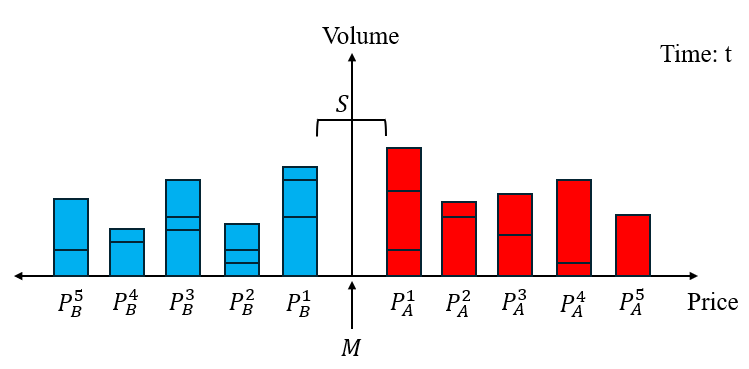
\includegraphics[width=0.8\linewidth]{figures/order_book_t.png}
    \caption{Limit Order Book Flow at Time $t$} 
    \caption*{\textit{Note:} The structure of the limit order book at time $t$, includes the first five levels on both the bid side ($P_B^1$ to $P_B^5$, in blue) and ask side ($P_A^1$ to $P_A^5$, in red). Each bar represents the volume of outstanding limit orders at the corresponding price level. The size of bars shows how large is the volume. $P_B^1$ is the best (highest) bid price, and $P_A^1$ is the best (lowest) ask price. The spread $S$ is defined as $P_A^1 - P_B^1$, and the midpoint $M$ is the average of the best bid and ask prices. Bid prices decrease with level, and ask prices increase. }
    \label{fig: order_book_t}
\end{figure}

From the perspective of buyers, placing orders in the bid range reflects a more neutral or passive opinion, as these orders wait to be matched rather than executed immediately. This provides liquidity to the market. Conversely, when buyers want to execute orders more aggressively, they place orders at the ask price range, increasing the likelihood of immediate execution. Aggressive buy orders take ask orders out of the order book flow and consume market liquidity. In other words, $P_A ^ {1}$ is the lowest price at which it is immediately possible to buy the traded asset. This also leads to a concept of \textit{market orders}, contrary to which are the \textit{limit orders}. Market orders stand for orders which are filled immediately after submission, while limit orders become the available liquidity active in the order book. However, aside from immediacy of execution, there is no fundamental difference between the two order types. The same mechanism applies to sellers, where passive sell orders provide liquidity at the ask price, while aggressive sell orders execute against bid prices.

The \textit{bid-ask spread} $S$ and \textit{mid-price} $M$ are fundamental metrics derived from the best bid price $P_B ^ {1}$ and best ask price $P_A ^ {1}$. Despite their mathematical simplicity, as expressed in Equations \ref{eq:spread} and \ref{eq:mid price}, these two metrics play a crucial role in the \gls{microstructure of financial markets}, much like how the Einstein field equations support the theoretical framework of general relativity. They serve as a bridge between market activity interface and the underlying mechanisms of price formation, liquidity, and trading dynamics. Every study on the limit order book certainly involves these measures, as they illustrate essential market characteristics.
\begin{align}
    S = P_A ^ {1} - P_B ^ {1}  \label{eq:spread}\\
    M = (P_A ^ {1} + P_B ^ {1})/2
    \label{eq:mid price}
\end{align}

The bid-ask spread is a key indicator of market liquidity and transaction costs. A narrower spread suggests higher liquidity and lower execution costs, while a wider spread may indicate market inefficiencies or heightened uncertainty \citep{GLOSTEN198571}. Moreover, changes in the spread are closely linked to market sentiment, as it tends to widen during periods of volatility and tighten when market conditions stabilize.

The mid-price, on the other hand, is a fair valuation across the order book flow. It serves as a benchmark for price movements and is widely used in empirical research to model order flow dynamics, volatility, and high-frequency trading strategies. Statistical properties, like stability and convergence, of mid-price provide insights into price simulation and prediction. More stylized facts are demonstrated in Chapter~\ref{cp: facts}. 

\subsection{Price Mechanism and Market Impact}
%how to match, how to fill, how to disappear, auction
In the limit order book, price matching mechanism take the lead of the evolution of bid/ask prices over time. The most common rule is that orders follow a \textit{price-time priority}, meaning higher bid prices and lower ask prices get matched first. When multiple orders are placed at the same price, they are executed following a first-come, first-served rule. 

When a limit order is placed, it is not immediately matched and stays in the order book, adding liquidity and waiting for future trades. When a market order is placed, it is executed at the best available price on the opposite side of the book. If the order is larger than the available volume at that price, the rest moves to the next best level until it is fully executed, or no more matches are found. 

To illustrate the order book flow more clearly, Figure~\ref{fig: order_book_t_1} shows the state of the book at time $t+1$, following Figure~\ref{fig: order_book_t}. When a buy limit order is placed at bid price level 1 ($P_B^1$), it means a trader wants to buy but prefers a better price over immediate execution. This order follows the time priority and remains active until either the market moves downwards or aggressive traders occur to take this order out directly. But the order can only be filled after all earlier orders at the same price level are filled or canceled. Such a passive limit order does not cause $\{P_B ^ {i}$, $i = 1, \dots, 5\}$ or $\{P_A ^ {i}$, $i = 1, \dots, 5\}$ to change. 

\begin{figure}[h]
    \centering
    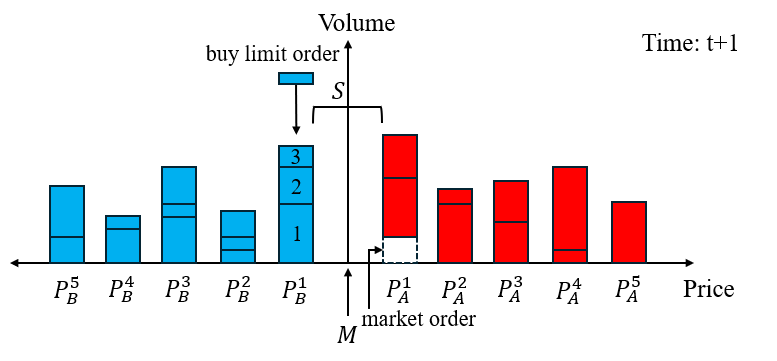
\includegraphics[width=0.8\linewidth]{figures/order_book_t_1.png}
    \caption{Limit Order Book Flow at Time t+1}
    \caption*{\textit{Note:} The state of the limit order book at time $t+1$, follows the submission of a passive buy limit order at the best bid price level $P_B^1$. The order joins the existing queue without changing the current bid or ask prices, $\{P_B^i\}_{i=1}^5$ and $\{P_A^i\}_{i=1}^5$. The order remains active until it is matched by an incoming market sell order or cancelled. At $P_A^1$, a market order consumes the bottom order due to price-time priority.}
    \label{fig: order_book_t_1}
\end{figure}

There is also a market order filled at ask price level 1 ($P_A^1$) in Figure~\ref{fig: order_book_t_1}. This represents a trader who wants to buy aggressively, matching against the highest priority active sell order in the order book. As a result, it is executed immediately at $P_A^1$. Whether the best ask price ($P_A^1$) changes depends on how big the market order is compared to the number of active sell orders at $P_A^1$. If the market order is larger than the available sell volume at this price, the remaining part of the order will continue to match with the next best ask price ($P_A^2$), and then $P_A^3$, and so on. The process will continue until the entire order is filled. But in the case that there is a no-worse-than price applied to the market order, the process will end when there are no more sell orders at reasonable prices. If all the sell orders at $P_A^1$ are used up, the best ask price will move to the next available sell order ($P_A^2$) in the book. This means that large market orders can push prices up by removing sell orders at multiple levels.

Moreover, when a buy (respectively, sell) order is placed between best bid (respectively, ask) price and best ask (respectively, bid)price, it will cause the $\{P_B ^ {i}\}$ to move right and best bid price to increase (respectively, the $\{P_A ^ {i}\}$ to move left and best ask price to decrease). 

Other actions, such as canceling, changing, or placing new orders, along with order filling, constantly update the order book, influencing price movements and order book dynamics.

% \subsection{Stylized Facts} \label{cp: facts}
% %heavy-tailed, volatility clustering, long memory in order flow, autocorrelation, Brownian motion of mid-price
% As mentioned at the end of Chapter 1.1.1, the limit order book exhibits various statistical properties which are the so-called \textit{stylized facts}. \cite{vyetrenko_get_2019} reviewed a wide range of stylized facts, but I focus on a concise subset that is the most relevant to limit order book simulation:
% \begin{enumerate}
%     \item Arrival rates: Orders do not arrive randomly but follow patterns. The frequency of order arrivals follows statistical patterns and is commonly modeled using point processes.
%     \item Autocorrelation of price changes: Price changes tend to slightly reverse in the short term due to bid-ask spread effects, but over longer periods, price changes are mostly independent.
%     \item Volatility clustering: When prices move a lot in one period, they tend to keep moving a lot in the next. When price changes are small, they stay small for a while.
%     \item Heavy-tailed distributions: The distribution of price returns, order sizes, and waiting times exhibits heavy tails. Extreme values price movements happen more often than expected in a normal distribution.
%     \item Average shape of the book: The number of buy and sell orders at different price levels is not balanced. Some price levels have more orders than others, creating a typical shape.
%     \item Price paths: Prices do not move randomly but follow patterns influenced by order flow. Over long periods, mid-price is convergent to a Brownian motion in a complete limit order book. 
%     \item Long memory in order flow: Buy and sell orders are not placed randomly. The way orders are placed, canceled, and executed depends on past order activity and follows long-term patterns.
% \end{enumerate}


\subsection{Challenges in Limit Order Book}
Due to the high frequency of trading, the presence of algorithmic strategies, and the participation of multiple traders, studying \gls{lob} is difficult. There are various problems challenging the analysis. \cite{drame2020limitorderbooklob} thinks the presence of both informed and uninformed traders causes information asymmetry on \gls{lob} dynamics. \cite{gould_limit_2013} further discuss the balance between perfect rationality and zero intelligence when describing trader behavior. However, this section focuses on the structural and operational challenges of the \gls{lob} itself, particularly those that affect simulation and its application in back testing trading strategies.
\begin{enumerate}
    \item State-space complexity: The \gls{lob} has a huge number of possible states at any given moment. The continuous updates of orders results in a dynamic system with high-dimensional complexity, which increases the computationally difficult. To make analysis feasible, simplifying assumptions are necessary. But preserving essential structures and statistical properties of the \gls{lob} is also indispensable.

    \item Incomplete order book along with aggressive trades: The visible limit order book does not show all trading intentions. Additional transaction details exist in trade book data, which are not reflected in the standard order book view. On the one hand, it's because some \gls{venues} allow traders to submit hidden-size orders that do not appear in order book updates. But these hidden passive orders are not important in our backtesting. On the other hand, aggressive trading events shot specific orders immediately. Such orders tend to be market orders, directly taking active orders out. As a result, researcher can't make sure that the observed \gls{lob} are actually the real activities happening in the realistic market. To address this issue, trade book data can be compared with order book records to identify missing events, and efforts can be made to reconstruct the true order flow by incorporating aggressive trades.

    \item Cancellation: Studies have indicated that most orders end in cancellation rather than filling. This seems to show a high level of trader disappointment. However, cancellations are not always due to unfulfilled intentions, some traders place and then cancel orders on purpose in order to gauge market trends and hidden liquidity. The meaning of volume changes in the \gls{lob} vary: some orders are fully or partially filled, some are canceled, and others remain unchanged. These possibilities contribute to the complex volume dynamics at each price, making it difficult to distinguish order filling from cancellation. Trade book data is crucial in addressing this issue, as it provides additional information on whether volume changes result from actual trades or cancellations.

    \item Differences among venues: The \gls{lob} updates are different across venues due to variations in market structure and transparency. Some venues allow more hidden orders and do not provide detailed order messages, making it harder to reconstruct the full order flow. Moreover, rules about the order book types vary significantly from one venue to another.
    About liquidity, some venues provide \textit{firm liquidity}, meaning that once an order is matched, it becomes a trade. In contrast, others offer \textit{last look liquidity}, where even if an order is matched, the liquidity provider or market maker can reject the trade. For example, the market price changes right after the match. In theory, last look liquidity venues tend to have a smaller bid-ask spread compared to firm liquidity venues.
\end{enumerate}

% \section{Algorithmic Execution}
% 1. different types

% Time Weighted Average Price aims to execute a given order in a given time frame and approach the time weighted average price during this time frame.

% Volume Weighted Average Price




\section{FX Smart Order Execution Platform}
MN is a Netherlands-based company that provides services to pension funds and other institutional investors. MN works closely with its clients to help them reach their long-term goals. What makes MN stand out is its strong understanding of pensions and the practical challenges that pension fund boards face. In order to offer more reliable and innovative investment solutions, MN has developed the FX Smart Order Execution Platform (Algo), an automated execution engine that can perform algorithmic execution of orders in the FX spot market. By building this automatic execution platform, they managed to lower trading costs which was used to pay for the banks. Also, this platform helps traders have more transparent decision-making power. They can literally decide the trading strategies and execution algorithms.

\subsection{Application Infrastructure}
The platform has a modular design, cloud infrastructure, and exchange connectivity. It includes three main components: the frontend, which features a graphical user interface (GUI); the backend, which is hosted on Amazon Web Services (AWS); and the smart execution engine, which operates on a remote server located in London.
% The work flow of the platform is shown in Fig.~\ref{fig:application infrastructure}. 

% \begin{figure}[h]
%     \centering
%     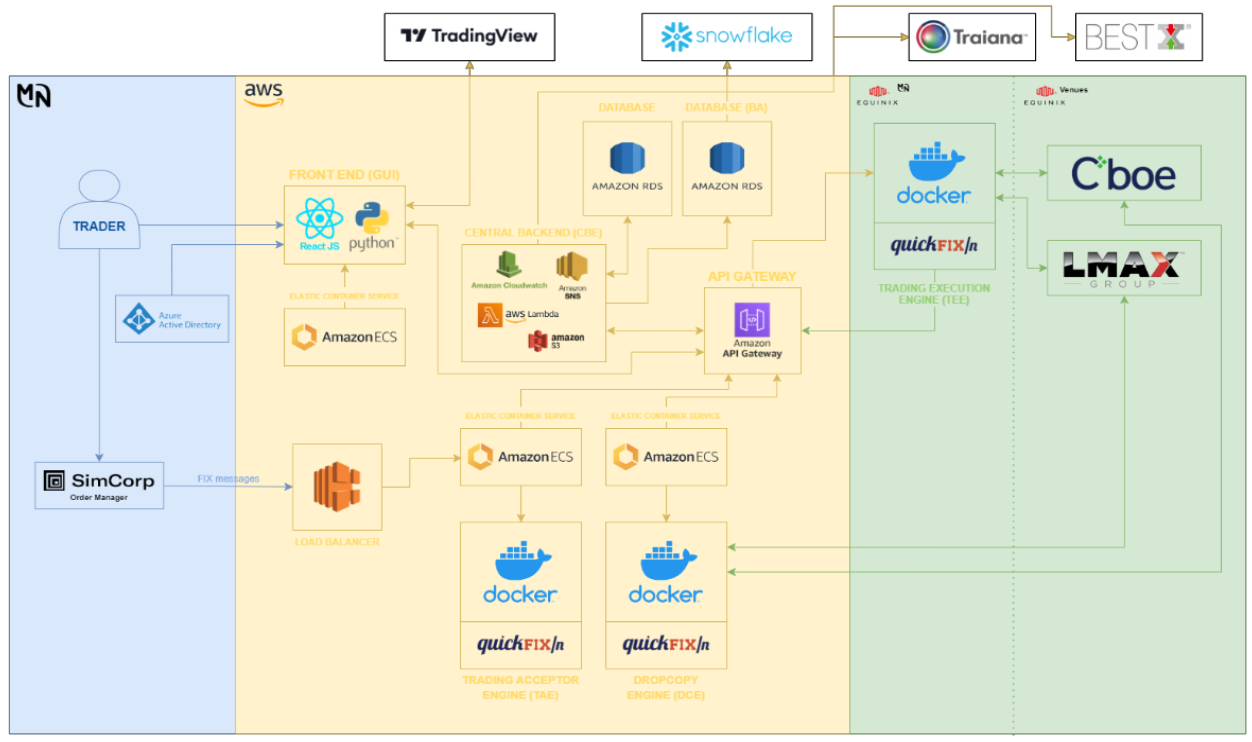
\includegraphics[width=\linewidth]{figures/Application Infrastructure.png}
%     \caption{Application Infrastructure of Algo}
%     \label{fig:application infrastructure}
% \end{figure}

The frontend, built with ReactJS and Python, provides an interface for traders and runs on AWS. Orders are processed through SimCorp Order Manager and authenticated via Azure Active Directory. The backend, hosted on AWS, handles data processing, trade execution, and market data storage using Amazon RDS and S3. It connects to the frontend and external services through an API gateway. The trading execution engine operates on Equinix, using Docker and QuickFIX/n for low-latency order processing. It connects to major venues like Cboe and LMAX Group. The system also integrates TradingView for market data, Snowflake for data storage, and Traiana and BestX for trade reconciliation and cost analysis.

\subsection{Execution Algorithm}
Putting a large order in the market all at once could result in unwanted high market impact and high costs, so instead, an order (parent order) is divided into multiple smaller child orders. These child orders are then executed according to the specific algorithm chosen by the trader. As long as child orders are not filled, they are refreshed every 50 milliseconds. 

Two execution algorithms are implemented in the Algo trading pool. They can take orders aggressively out of the order book at a certain price with a market order (resulting in spread costs) or can place limit orders in the order book, passively waiting for the order to be executed at a favorable price (resulting in opportunity costs). To maintain efficiency, child orders are refreshed every 50 milliseconds, updating their price according to market conditions while staying within the predefined limit price $L$. If the refreshed price exceeds the limit price, the order remains pending until the next update.

One algorithm is Time Weighted Average Price (TWAP) algorithm. This algorithm replicates traditional TWAP, but uses parameters to control passive, neutral and aggressive execution of child orders. It is designed to execute a trade over a fixed time period while aiming to match the time-weighted average mid-price. It splits a large order into multiple smaller child orders that are executed parallelly to minimize market impact and reduce price deviation.

TWAP algorithm requires four main inputs: the start time $t_0$, the total order volume $Q$, the execution duration $T$, and the limit price $L$. The TWAP price is defined as the time-weighted integral of the mid-price $M(t)$ over the trading period:

\begin{equation}
    p_{\text{TWAP}} = \frac{1}{T} \int_{t_0}^{t_0+T} M(t) dt.
    \label{eq: TWQP price}
\end{equation}

To approximate this price, the algorithm partitions the total volume into $n$ child orders, where $n$ is determined by the ratio of $Q$ to the minimum allowed child volume $Q_{\min}$:

\begin{equation}
    n = \left\lfloor \frac{Q}{Q_{\min}} \right\rfloor, \quad Q_n = Q - (n-1) Q_{\min}.
    \label{eq: Q_n}
\end{equation}

Each child order follows a randomized start time to reduce signaling risk. A random value $a_i$ is assigned to each child within a predefined range, and the duration of each child order is computed as:

\begin{equation}
    \delta_i = \frac{a_i T}{A}, \quad A = \sum_{i=1}^{n} a_i.
    \label{eq:sigma and A}
\end{equation}

The execution of each child order follows an adaptive approach, starting with a passive strategy and increasing aggressiveness over time. The aggressiveness is controlled by three parameters: $\alpha$, $\beta$, and $\gamma$. The order initially starts at $\alpha$ and, if unfilled, transitions to $\alpha + \beta$ after a fraction $t_{\beta}$ of its duration. If the order remains unfilled, the price fraction further increases to $\alpha + \beta + \gamma$ at time $t_{\gamma}$.

% \begin{table}[h]
%     \centering
%     \begin{tabular}{|c|l|}
%         \hline
%         \textbf{Symbol} & \textbf{Description} \\ \hline
%         $\alpha$ & Initial price fraction \\ \hline
%         $\beta$ & Increment for the second phase \\ \hline
%         $\gamma$ & Increment for the third phase \\ \hline
%         $t_{\beta}$ & Time fraction before increasing aggressiveness \\ \hline
%         $t_{\gamma}$ & Time fraction before final aggressiveness step \\ \hline
%     \end{tabular} \label{tb:TWAP parameters}
%     \caption{TWAP execution parameters}
%     \caption*{\textit{Note:}}

% \end{table}

In the passive mode, orders begin at $\alpha$ and transition through all phases. The neutral mode omits the passive phase and starts at $\alpha + \beta$, while the aggressive mode starts directly at the highest level of aggressiveness. This approach ensures the order is executed in a controlled manner while adapting to market conditions, reducing the risk of price deviation and improving execution efficiency.

Figure~\ref{fig:order placement} shows the definition of order aggressiveness of Algo.

% order placement picture in the ppt
\begin{figure}[h]
    \centering
    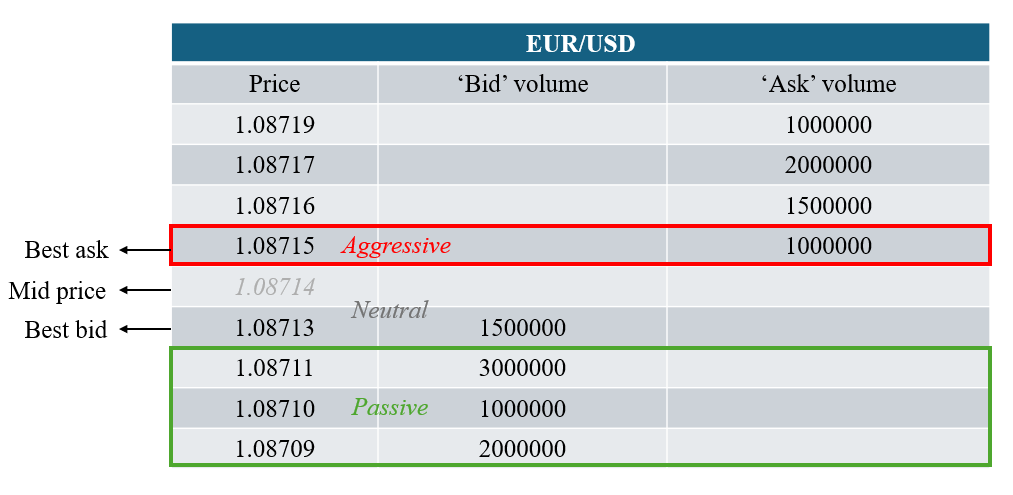
\includegraphics[width=\linewidth]{figures/order placement.png}
    \caption{Order placement for buyers of Algo}
    \caption*{\textit{Note:} Demonstration of traders who want to buy orders. Aggressive order is placed at the best ask. Neutral order is placed at the mid-price or best bid. Passive order is placed near the best bid.}
    \label{fig:order placement}
\end{figure}

The other one is Float algorithm. Different from TWAP, it lets the child order 'float' at a specific price level until executed. This approach reduces market impact and lowers spread costs. Since execution speed is not a priority, the algorithm is categorized as a \textit{liquidity-seeking} strategy. This algorithm allows child orders wait passively at a predefined level in the order book and adjusts its position dynamically.

The Float algorithm requires the following inputs:
\begin{itemize}
    \item A start time $t_0$.
    \item A total order volume $Q$.
    \item A price fraction $\phi$, which defines the floating position in the order book.
    \item A limit price $L$, ensuring the order does not execute at an unfavorable price.
\end{itemize}

The execution process begins by setting the remaining volume $R = Q$. The algorithm then continuously executes child orders until the total volume is filled. The volume of each child order is determined dynamically using the remaining volume:

\begin{equation}
    Q = 
    \begin{cases} 
        Q_{\text{float}}, & \text{if } R - Q_{\text{float}} \geq Q_{\text{float}}, \\
        R, & \text{otherwise}.
    \end{cases}
\end{equation}

Each child order keeps the same price fraction $\phi$ throughout its lifespan. Orders are refreshed every 50 milliseconds to ensure they remain valid under current market conditions. If a child order executes too quickly, the algorithm enforces a minimum execution duration $\delta_{\text{min}}$, delaying the next child order until sufficient time has passed.

In some cases, the market may move beyond the limit price, preventing further execution. If this happens, the order becomes stuck, meaning it will not execute unless the market returns to a favorable level. To prevent unfilled orders from persisting indefinitely, any remaining float orders are canceled at the end of each trading day.

The key differences between Float and TWAP are:
\begin{enumerate}
    \item Dynamic Timing: In TWAP, child orders have pre-defined execution times, while in Float, a new child order is only created when the previous one is filled.
    \item Remaining Volume Handling: In TWAP, unfilled portions of child orders are added to the last order. In Float, unfilled portions are returned to the remaining volume and used to calculate the next child order.
\end{enumerate}

\subsection{Parallel Venue Submission}
The MN Algo uses two trading venues: \acrshort{lmax} and \acrshort{cboe}. These venues provide real-time market updates at the millisecond level, ensuring that trading decisions are based on the most recent market conditions. 

When a trader submits an order, the execution engine determines the venue for submitting the child order. To make order submission more efficient, parallel execution is implemented to meet the business need for higher trading volume and faster execution while keeping stable spreads.

The venue submission algorithm has experienced four stages of evolution. Initially, the algorithm submitted orders to the venue with the worst best bid/ask prices. This method made sure orders are placed in the less competitive venue, so they can be filled as soon as possible. But it did not optimize execution speed or market impact. The process is illustrated in Figure~\ref{fig:venue_submission_1}, where the parent order is divided into child orders, and each child order is sent to a single venue depending on the best bis/ask prices.

\begin{figure}[h]
    \centering
    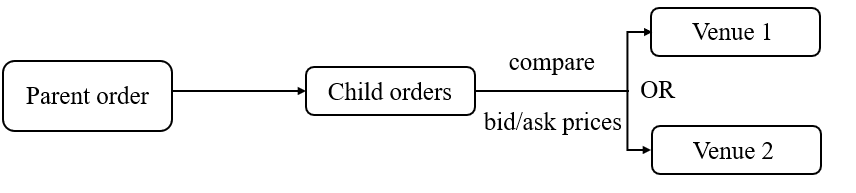
\includegraphics[width=0.8\linewidth]{figures/venue_submission_1.png}
    \caption{Initial venue submission method}
    \caption*{\textit{Note:} First version of parallel execution split the parent order into a set of child orders. Then child orders are sent to different venues after comparison of the bid/ask prices.}
    \label{fig:venue_submission_1}
\end{figure}

A later study \citep{romy2023} found that randomly selecting a venue for each child order resulted in better performance. This randomization changed the systematic disadvantages of initial method, leading a better execution performance. Further refinement is the use of \gls{parallel execution}, which significantly improved the performance of venue submission. Instead of submitting a single child order at a time, the algorithm places multiple child orders simultaneously across different venues. 

The first version of parallel execution split the parent order into multiple secondary parent orders, each assigned to a specific venue. Figure~\ref{fig:venue_submission_2} shows its execution process. If only one secondary order remains active, the algorithm reverts to the previous random execution method to prevent delays and ensure timely order completion. 

\begin{figure}[h]
    \centering
    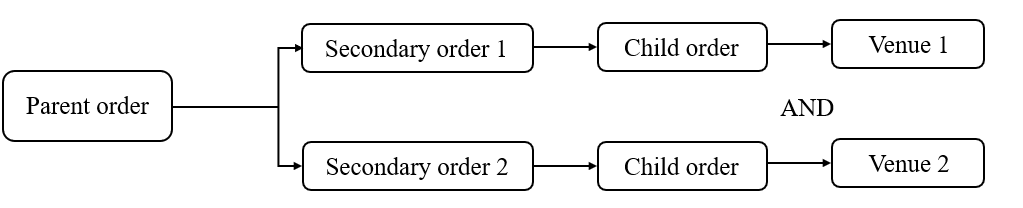
\includegraphics[width=0.8\linewidth]{figures/venue_submission_2.png}
    \caption{Parallel execution strategy version 1}
    \caption*{\textit{Note:} The parent order is split into two secondary orders. Each secondary order creates its own child order for execution. The two child orders are processed in parallel at Venue 1 and Venue 2. If only one secondary order remains active, the strategy switches to a random single-venue execution to reduce delay and complete the order on time.}
    \label{fig:venue_submission_2}
\end{figure}

Building upon this, the second version of parallel execution adjusts order execution dynamically based on venue performance. Since each venue or secondary order may have different execution speeds, the algorithm monitors execution at predefined intervals, referred to as pillars, and modifies execution settings in response to key triggers such as volume, price, and spread. The execution process is shown in Figure~\ref{fig:venue_submission_3}.
\begin{figure}[h]
    \centering
    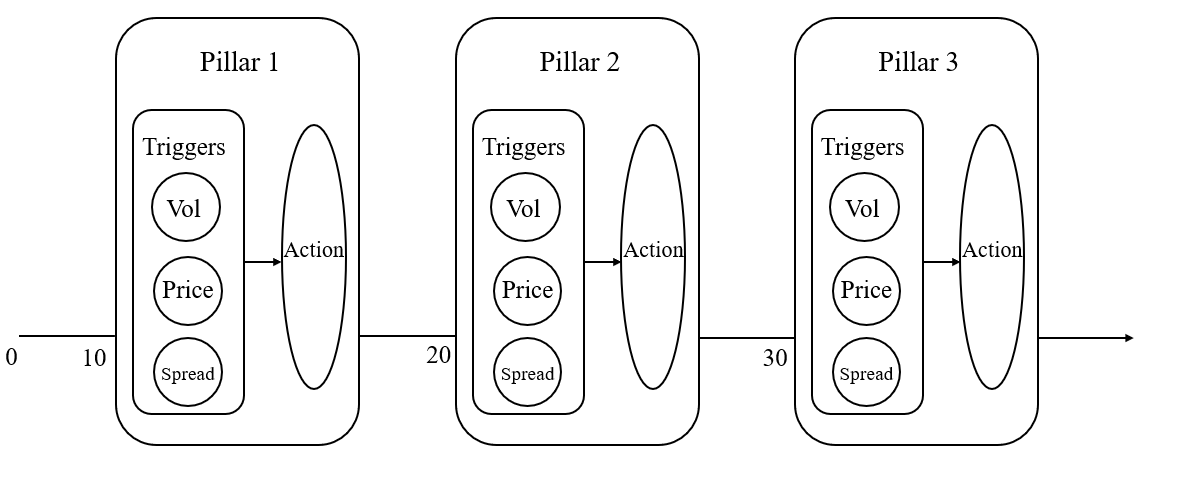
\includegraphics[width=0.8\linewidth]{figures/venue_submission_3.png}
    \caption{Parallel execution strategy version 2}
    \caption*{\textit{Note:} Three monitoring stages, called Pillars, each represents a predefined time point (e.g., 10, 20, 30 seconds) where venue performance is evaluated. The triggers (volume, price and spread) are used to decide the next action. This version reacts to real-time market conditions compared to version 1 and is currently used in the Algo.}
    \label{fig:venue_submission_3}
\end{figure}

% The transition from single-venue submission to randomized venue selection and ultimately to parallel execution has led to more efficient order processing, lower latency, and improved fill rates. Current parallel venue submission ensures that the trading strategy adapts to dynamic market conditions and optimizes execution quality.


\section{Back Testing}
Backtesting is a fundamental method used in quantitative trading to evaluate the performance of trading strategies based on historical market data. By predicting past trading conditions, backtesting provides evaluation of a strategy's performances before using it in live markets. A reliable backtesting environment should be both \textbf{realistic} and \textbf{dynamic}.

Companies have various systems for backtesting. MN has developed a back testing environment for FX spot trading, called \textit{FX Smart Execution Backtester} (referred to as the \textit{backtester} hereafter). This engine is designed to assess the performance of changes in execution strategy parameters, including the optimization of child order aggressiveness and the changes of order information. 

% The backtester aims to make use of complete market data:
% \begin{enumerate}
%     \item Historical data: Past \gls{lob} from LMAX and CBOE stored in the Snowflake.
%     \item Simulated data: Synthetic \gls{lob} generated to test hidden aggressive events beyond observation.
%     \item Model data: Data produced by algorithmic models to enhance market simulations.
% \end{enumerate}
Currently, the backtester only uses historical LOB data to execute testing of strategies. The execution engine processes order updates, places child orders at certain timestamps, and decides the rules of order matching. The order matching rule is now based on filling possibility depending on spread. The mechanism is:
\begin{itemize}
    \item Given an order information, including price, volume, trading algorithm, starting time and backtesting time range.
    \item Use best bid-ask spread to decide the filling chance of each order. As can be seen in Table~\ref{tab:filling_spread}, the narrower the spread, the higher the chance of an order being filled.
    \item Execute the order based on historical order book data.
\end{itemize} 
    \begin{table}[h]
        \centering
        \caption{Filling Probability and Bid-Ask Spread}
        \caption*{\textit{Note:} The spread values are in pip units, where $S=1$ corresponds to $0.0001$. Thus, $S \geq 5$ means $S \geq 0.0005$. When $S \geq 5$, the possibility of orders getting filled is $0$. The same as the following situations. When $S < 1$, the filling possibility is the highest ($20\%$).}
        \begin{tabular}{c|c|c|c|c|c|c}
            \hline
            Spread & $S \geq$ 5 & $S \geq$ 4 & $S \geq$ 3 & $S \geq$ 2 & $S \geq$ 1 & $S <$ 1 \\
            \hline
            Possibility of orders being filled & 0\% & 0.50\% & 1\% & 2\% & 5\% & 20\% \\
            \hline
        \end{tabular}
        \label{tab:filling_spread}
    \end{table}



% So, whether an order would be filled or not is decided by market trend and other market participators under the simulated market order book flow. 

\chapter{Literature Review} \label{chapter:literature}
To position this study within the broader context of existing research, I begin by reviewing the relevant literature on limit order book modeling and aggressiveness analysis in Section~\ref{sec:relatedwork}. In Section~\ref{sec:maincontributions}, I discuss the main contributions of this thesis compared to related work of others. In Section~\ref{sec:researchobjectives}, the main purpose of the thesis is stressed.                                                                                  
\section{Related Work} \label{sec:relatedwork}
% [why the LOB is important to consider][high-frequenct][imbalance]
Today, limit order book (LOB) is important to consider and model. More than half of highly competitive financial markets use the LOB mechanism to match buy and sell trade \citep{lob2009}. The LOB records rich, detailed, and high-quality historic data \citep{gould_limit_2013}. LOB-related modeling work can help in many ways. It can give better ideas on how to trade in different market conditions \citep{SuperDOT1996}, choosing good order execution strategies \citep{OBIZHAEVA20131} and reducing market impact \citep{Eisler01092012}. \cite{cvitanic_high_nodate} studied the distribution of transaction prices generated in a LOB market populated by orders from high frequency traders (machines) and low frequency traders (humans). They confirmed the limit order book is central to understanding how different trader types affect transaction prices. These are the reasons that the LOB data is useful for testing theories about common patterns found across a wide range of markets, thus important in this thesis research contents. 

% [limit order book modeling] what they do, what they find
There are many works devoted to modeling limit order book data. These models are typically based on either classical stochastic processes, machine learning methods, or hybrid approaches. In this section, I summarize key contributions in the literature, highlight their targets and modeling methods, and point out their limitations. How our approach improves upon them is discussed in Section~\ref{sec:maincontributions}.

A popular direction in the previous work is to model the LOB using stochastic processes, such as Poisson processes, Hawkes processes, or Markov models. For example, \cite{cont_stochastic_2010} introduced a continuous-time stochastic model for the dynamics of a limit order book. This approach allows for analytical explanation but ignores clustering and feedback effects. 
\cite{bleher_orders_2021} proposed a Markov process LOB model. While it is theoretically rich, their model assumes exponential timing and lacks nonlinear pattern recognition.
\cite{lu_order-book_2018} analyzed and enhanced the original Markovian model based on non-Markovian features of empirical observations. The model adds dependency on past events, thus significantly improving the realism of LOB simulations and the profitability of market making strategies. 
Market and limit order flows play an important role in LOB modeling. \cite{bechler2017orderflowslimitorder} studied limit order book behavior over short timescales using volume-based data. They found that trade imbalance and price change are nonlinearly related, but this becomes linear when combining market and limit order flows. 
Regarding the clustering property, \cite{vinkovskaya_point_nodate} found orders and cancellations cluster in time, are interdependent, and influenced by the bid-ask spread by a self-exciting point process model with multiple regimes. But the model didn't consider more complex market features and dynamics.
A more mathematical modeling is done by \cite{cont_mathematical_2023}. They developed a general and flexible framework to model the dynamics of limit order books by combining two key components: order flow, modeled as a spatial point process (random arrival of buy/sell orders across price levels), and market clearing, represented as a 'mass transport' operator that matches orders. Their model brings together and extends earlier LOB models, making it easier to study how trades affect prices using math or simulations.
In high-frequent market, discrete models are helpful and effective. \cite{bayraktar_liquidation_2012} studied how to optimally sell a large position in a limit order book where order intensity depend on the price. They proved why discrete model is valid for LOB modeling by analyzing a continuous limit and showed that the discrete model's solution converges to the limit using viscosity solution techniques. 

Hawkes processes have become popular and useful because they can capture self-exciting behavior and clustering, which are vital properties in LOB. \cite{fonseca_clustering_2015} introduced clustering behavior captured by Hawkes process. However, these models usually assume static exponential kernels and cannot capture more complex dynamics. A Hawkes process-based LOB model is used by \cite{abergel_long-time_2015} highlight the long-time behaviour of the limit order book and the corresponding dynamics of the suitably rescaled price. \cite{zheng_ergodicity_2013} used multivariate Hawkes processes to model mutual excitations between market and limit orders. Their model captures self- and cross-exciting behavior, but the order flow kernels are still simple. \cite{lalor_algorithmic_2025} modeled LOB prices using semi-Markov and Hawkes jump-diffusion processes to capture jumps and clustering but lacks data-driven components and real feature inputs.

% [extensions of Hawkes process]
% \cite{kumar2021deephawkesprocesshighfrequency}
% \cite{magris_simulation_nodate}
% \cite{shi_neural_2023}

There are many extensions of traditional Hawkes process model. The Buffer-Hawkes model \citep{kaj_buffer_2017} extends the Hawkes process by including a buffer state that connects order flow with market executions. It models mutual excitation and execution feedback but is still limited to Markovian settings. Similarly, a LSTM-based Neural Hawkes Process \citep{lalor_event-based_2025} aim to generate realistic multi-event LOB environments for testing market-making strategies. These works are powerful but usually require a lot of computation and not suitable for high-frequent FX trading. Another extension of the Hawkes process is non-parametric marked Hawkes models \citep{joseph_non-parametric_2024}. They use neural networks to learn the kernel functions. This improves flexibility but requires a lot of data and computation.

% [machine learning tools]
\cite{coletta2021towards}
Machine learning methods are widely used in recent years. \cite{briola_deep_2024} uses convolutional and LSTM layers to predict mid-price movements. While it gives good accuracy, it lacks interpretability. Other works use GANs \citep{brophy_quick_2019} or Neural SDEs \citep{issa_non-adversarial_2023} to generate realistic time series, but training is often unstable and not efficient for high-frequency tasks. \cite{huang_simulating_2014} proposed the queue-reactive model. This approach is simple and gives good estimates of execution probability and market impact, but it ignores deeper temporal patterns.

% other fields
% \cite{esteban_real-valued_2017}
% \cite{brophy_quick_2019}

To evaluate the quality of simulations, \cite{vyetrenko_get_2019} introduced realism metrics that test both macro and micro features. This work shows that many GAN-based simulators lack realism and produce agents that fail when tested on real markets. This is the reason that I do not apply GANs in our study. Even though it has strong generation ability, reality is an important factor for our model.



% [why the study of aggressive trades is interesting]
Other empirical works analyze order placement and aggressiveness. A key reason for studying the aggressive trade in LOB is that it connects individual trading activity with overall price dynamics. \cite{xu2019multilevelorderflowimbalancelimit} found how order-flow activity deep into the LOB can influence the price-formation process by trade imbalance and order-flow Imbalance modeling. More specifically, \cite{OrderAggressiveness2010} found that more aggressive orders are usually smaller. When there are many orders on the same side, traders place smaller and less aggressive orders. But when the other side is deeper, they place larger and more aggressive ones. The finding also shows the volume ratio is a critical factor when modeling aggressiveness, which will be considered in next modeling. 
% \cite{chiu_order_2017}
% \cite{HUNG2019231}
% \cite{RANALDO200453}





\section{Main Contributions} \label{sec:maincontributions}
While previous studies have made significant progress in understanding [briefly summarize what's been done], important gaps remain — particularly in terms of [highlight the limitation]. This thesis addresses these gaps and contributes to the literature in the following ways. In the literature review section, popular LOB models in the literature often rely on fixed stochastic structures or black-box machine learning, typically ignoring important market features, temporal dependency, clustering, and interpretability. For instance, models based only on single Hawkes processes cannot capture nonlinear relations in market conditions. On the other hand, deep learning models like GANs or LSTMs are hard to interpret and expensive to train.

In this thesis, I propose a novel approach that integrates a GRU-based Neural Hawkes Process with XGBoost to solve extreme class imbalance. It captures not only market features (e.g., spread, volume, imbalance), but also temporal dependencies and clustering behavior. Moreover, GRU is lighter than LSTM and more efficient for high-frequency data. Compared to GANs, it is easier to train and more stable. Compared to traditional Hawkes models, it is more flexible and dynamic. Compared to pure machine learning, it is not a black box and the intensity function has clear structure. It is fair to expect our method provides a better framework for predicting pattern of the aggressive trade.

\section{Research Objectives}\label{sec:researchobjectives}
% Define the limitations of existing backtesting frameworks, particularly their inability to capture realistic market responses.
Based on these contributions, we formalize the research objectives of this thesis. These objectives guide the development of our methodology and the design of our empirical analysis.
% Our mission starts from a company needs...
As discussed in the last section, the MN backtester is only based on historical \gls{lob} and simple filling possibility rules to match order. A big problem is that the filling possibilities cannot capture the sophisticated what-if scenarios accurately, like when market conditions differ, how trader's behaviors will change. This is especially intractable when back testing the execution of passive child orders, because they require aggressive market participants to trade through the spread and remove them from the order book. I can't know when aggressive trades take place only from current \gls{lob}, whether on LMAX or CBOE. The issue is even more obvious in CBOE, as it allows for a greater number of trading activities that do not appear in order book updates, further decreasing the backtesting accuracy. 

Hence, the objective of this thesis is to improve the MN backtester from the aspect of predicting if other market participants would aggressively take out our passive orders from the order book. The main idea involves developing models to analyze the distributional pattern of aggressive trades in real \gls{lob} dynamics. This will mimic the real market reaction to changes in the execution strategies. A naive idea would be to insert these aggressive trades randomly throughout the updates of order book. However, a more realistic and dynamic approach need to consider the self-exciting, clustering properties and distribution of aggressive trades, including how frequently they occur, under what conditions, and how they interact with existing order flow.

The challenge then becomes determining the distributional pattern of aggressive trades in the \gls{lob}. By addressing this, I can create a more realistic and dynamic backtesting mechanism. For further research, it would be interesting to see if the new backtesting mechanism can be applied in general backtesting frameworks for multiple assets and instruments like the FX swaps and equities market.



\chapter{Data} \label{chapter:preliminary}
This Chapter presents the data sources, data fetching method, initial description of the raw data, as well as data analysis and visualization methods. For demonstration, I use the dataset includes limit order book data, market trade book data and MN trade book data from 10:00:00 to 15:59:59 on 31st January as examples. The timestamps in the order book and MN trade book are recorded in London time, while those in the market trade book are American time. To ensure orders in order book are consistent with trades in trade book, all of them are converted to Central European Time (CET). As a result, both them represent for trading time between 10:00:00 and 15:59:59 CET. 

In Section~\ref{sec:data-source}, data structures are shown in tables, alongside brief description and data type. Then in Section~\ref{sec:match-order-trade}, I describe how trades in the trade book are matched with the orders in the order book. I build an algorithm to find this match by comparing trade prices and directions with the prices in different levels of the order book. I also classify visible trades into passive and aggressive types based on whether the match happens at the best bid/ask price. 
In Section~\ref{sec:price}, I explain the trading activity using the price and filling information from order book and trade book data. 


\section{Data Source and Types} \label{sec:data-source}
The order book dataset consists of foreign exchange (FX) limit order book data provided by LMAX and CBOE, two venues used by MN. Orders from LMAX is more transparent because LMAX is optimized for order-driven market model, while there are more latent orders in CBOE because of the support for anonymous trading. 

As can be seen in Table~\ref{tb: order book data description}, the currency type is EUR/USD. The data is detailed in bid/ask prices and volumes at 5 levels in total, where the data of level 1 stand for the best bid/ask. The dataset also calculates the spread between best ask and best bid prices.

All the order book data is stored in Snowflake, a cloud-based data platform that provides data storage, processing, and analytics as a fully managed service. High-frequency order book data can be accessed using SQL queries, which ensures high availability and completeness of data.

Table~\ref{tb: trade book data description} provides information of trade price, volume, execution time, and order direction in the trade book. Importantly, the order book is significantly larger than the trade book. For a single trading day, the order book can reach around 200,000 KB, while the trade book is typically only about 100 KB.


\begin{table}[ht]
    \centering
    \caption{Order Book Data Description}
    \caption*{\textit{Note:} All the entries in the order book data extracted from Snowflake. The ID is unique for every order. Timestamps are in millisecond. Venue 1 and venue 2 are two venues for FX trading at MN. The currency objective is EUR/USD. The following rows are volumes, price (all five levels) and spread.}
    \begin{tabular}{lll}
        \toprule
        \textbf{Column} & \textbf{Description} & \textbf{Data Type} \\
        \midrule
        ID & Unique identifier of orders & String \\
        $T$ & Time of the snapshot in HH:MM.SSS format & String \\
        VENUE & The exchange (venue 1 or venue 2) & String \\
        SYMBOL & Currency pair (EUR/USD) & Datetime \\
        $V_A$ & Total volume on the ask side & Integer \\
        $V_B$ & Total volume on the bid side & Integer \\
        $P_A ^ {i}$, $i = 1, \dots, 5$ & Ask prices at different levels & Float \\
        $V_A ^ {i}$, $i = 1, \dots, 5$ & Corresponding volumes at each ask level & Integer \\
        $P_B ^ {i}$, $i = 1, \dots, 5$ & Bid prices at different levels & Float \\
        $V_B ^ {i}$, $i = 1, \dots, 5$ & Corresponding volumes at each bid level & Integer \\
        $S$ & Difference between best ask and bid (S = $P_A ^ {1}$ - $P_B ^ {1}$) & Float \\
        \bottomrule
    \end{tabular} 
    \label{tb: order book data description}
\end{table}

\begin{table}[ht] 
    \centering 
    \caption{Trade Book Data Description}
    \caption*{\textit{Note:} All the entries in the trade book data extracted from Snowflake and exchanges database. Timestamps are in millisecond. Direction includes bid/ask. Prices are the filling price taking place when execution. Volumes are the number of orders traded.}
    \begin{tabular}{lll} 
        \toprule 
        \textbf{Column} & \textbf{Description} & \textbf{Data Type} \\ 
        \midrule 
        $T$ & Execution time of the trade (HH:MM:SSS) & String \\
        DIRECTION & Bid order or ask order & String \\
        PRICE & Execution price of the trade & Float \\ 
        VOLUME & Number of units traded & Integer \\  
        \bottomrule 
    \end{tabular} 
    \label{tb: trade book data description}  
\end{table}

\section{Matching Trade Book and Order Book Data} \label{sec:match-order-trade}
In an order-driven market, trades occur when incoming orders match existing orders in the order book. In the LOB, 'bid' represents buy interest, and 'ask' represents sell interest. When a trade is recorded in the trade book, it has a direction. If the direction is 'bid', it means the buyer placed an order that matched an existing ask order in the order book. In this case, the trade price corresponds to the ask price available in the order book at the time of execution, and the volume of the matched ask order decreases by the traded amount. If the direction is 'ask', it means the seller placed an order that matched an existing bid order in the order book. The trade price in this case corresponds to the bid price available in the order book, and the volume of the matched bid order decreases by the traded amount. The order book is updated after each trade to reflect the reduced volume of the matched order. If an order in the order book is fully consumed, it is removed. If there is remaining volume after a partial match, the order stays in the book with the updated volume. 

An algorithm is developed to find roots of trade book updates in the order book data. This is an important preliminary to see how orders in the order book get filled, which is important in back testing. Also, it is clear to see how many unmatching orders in the order book are. The algorithm for matching orders and trades is in Algorithm~\ref{alg:trade_order_matching}.

\begin{algorithm}
    \caption{Matching Trade Book and Order Book Data}
    \label{alg:trade_order_matching}
    \begin{algorithmic}[1]
        \State Load trade book (timestamp, price, volume, direction)
        \State Load order book (timestamp, price levels, volumes)
        \State Transform order book to long format (one row per price level)
        \State Merge and sort trade book and order book by timestamp
    
        \For {each trade}
            \State Find earlier matching limit orders
            \If {no matching order exists}
                \State Mark as hidden order
            \Else
                \State Check if buy trade matches ask or sell trade matches bid
                \State Record matched price level and traded volume for updates in trade book
                \State Record filling time and traded volume for updates in order book
            \EndIf
        \EndFor
    
        \State Define visible orders: trades that match existing limit orders
        \State Define hidden orders: trades with no matching limit order
        \State Define aggressive orders: visible trades not at best bid/ask
        \State Define passive orders: visible trades at best bid/ask
    
    \end{algorithmic}
\end{algorithm}

It starts by loading and filtering data. To identify matching trades, the algorithm checks whether each trade price appears in the five bid/ask levels of the order book. Since order book data stores prices and volumes separately, it is melted into a long format, aligning price levels with corresponding volumes. Then the trade book and order book are then merged into a complete order-trade dataset to accelerate direct comparison.

For each trade, the codes find previous orders in the order book, and check if price and direction match. The bid in the trade book should match the ask in the order book, the ask in the trade book should match the bid in the order book. As the result, If a trade matches an order, it is a visible execution. But if the matching price level is not the best bid or ask, it's identified as a passive submission getting filled by either market movements or aggressive market order. Further classification about these two scenarios will be done later in the chapter 4. If a trade cannot find its root in the order book, it's hidden orders, but I don't really care about this part.

As can be seen in the pie chart \ref{fig:p_of_AT_unma}, hidden trades only account for 3.5\%. Most trades are visible, which shows the high data quality from the exchange. Passive submission and neutral submission are both visible trades which I can find in the order book. Half of them are rooted as passive submission, which shows half traders are willing to queue in the order book flow and either wait for market movements or being chosen by aggressive traders. Half of the filling orders are placed in best bid/ask, meaning they prefer to be on top to get filled. This aligns with our trading strategies because most of our orders are placed passively or neutrally. I need to do modeling to predict how these orders get filled in the order flow. The second pie chart in Figure~\ref{fig:p_of_AT_unma} also confirms a common sense that 99\% of the orders in the order book cannot find their right trade and end in cancellation \citep{gould_limit_2013}. This phenomenon implies a potential extreme imbalance between aggressive and non-aggressive trades in the context of the overall order flow, which should be carefully considered when modeling trading patterns.

\begin{figure}[h]
    \centering
    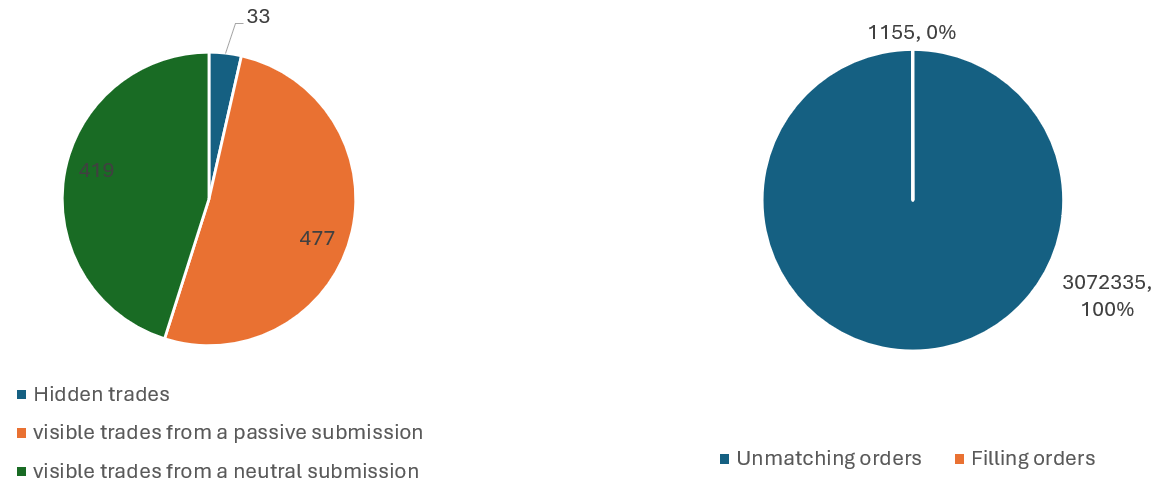
\includegraphics[width=0.8\linewidth]{figures/percentage_of_AT_unmatch.png}
    \caption{Percentage of Passive and Neutral Orders getting filled in the Trade Book and Orders Filled vs. Unmatched in the Order Book}
    \caption*{\textit{Note:} The left pie chart shows the breakdown of trades based on submission type. Only 3.5\% of trades are hidden, while the rest are visible and can be tracked in the order book. Among visible trades, roughly half come from passive submissions and half from neutral ones, indicating that many traders are willing to queue and wait for execution. This chart matches the behavior of FX trading strategies, which mostly use passive or neutral orders. The right pie chart shows the outcome of all limit orders submitted to the book. About 99\% of them are unmatched and end in cancellation, while only a small fraction result in executed trades.}
    \label{fig:p_of_AT_unma}
\end{figure}


\section{Prices and Filling Information} \label{sec:price}
To have a comprehensive understanding of how trades in trade book correspond to orders in order book, Figure~\ref{fig:p_f_i} provides an overview of the whole active trading hours from 10 am to 4 pm on 31st January. This date is chosen for demonstration, and the time window is the active trading time range during the day. This plot shows how filled price in the trade book track the mid-price in the order book, the distribution of passive and aggressive trades, and the spread range for each trade (not each order). The lower subplot presents the filled volume for each trading record.

% \begin{figure}[ht]
%     \centering
%     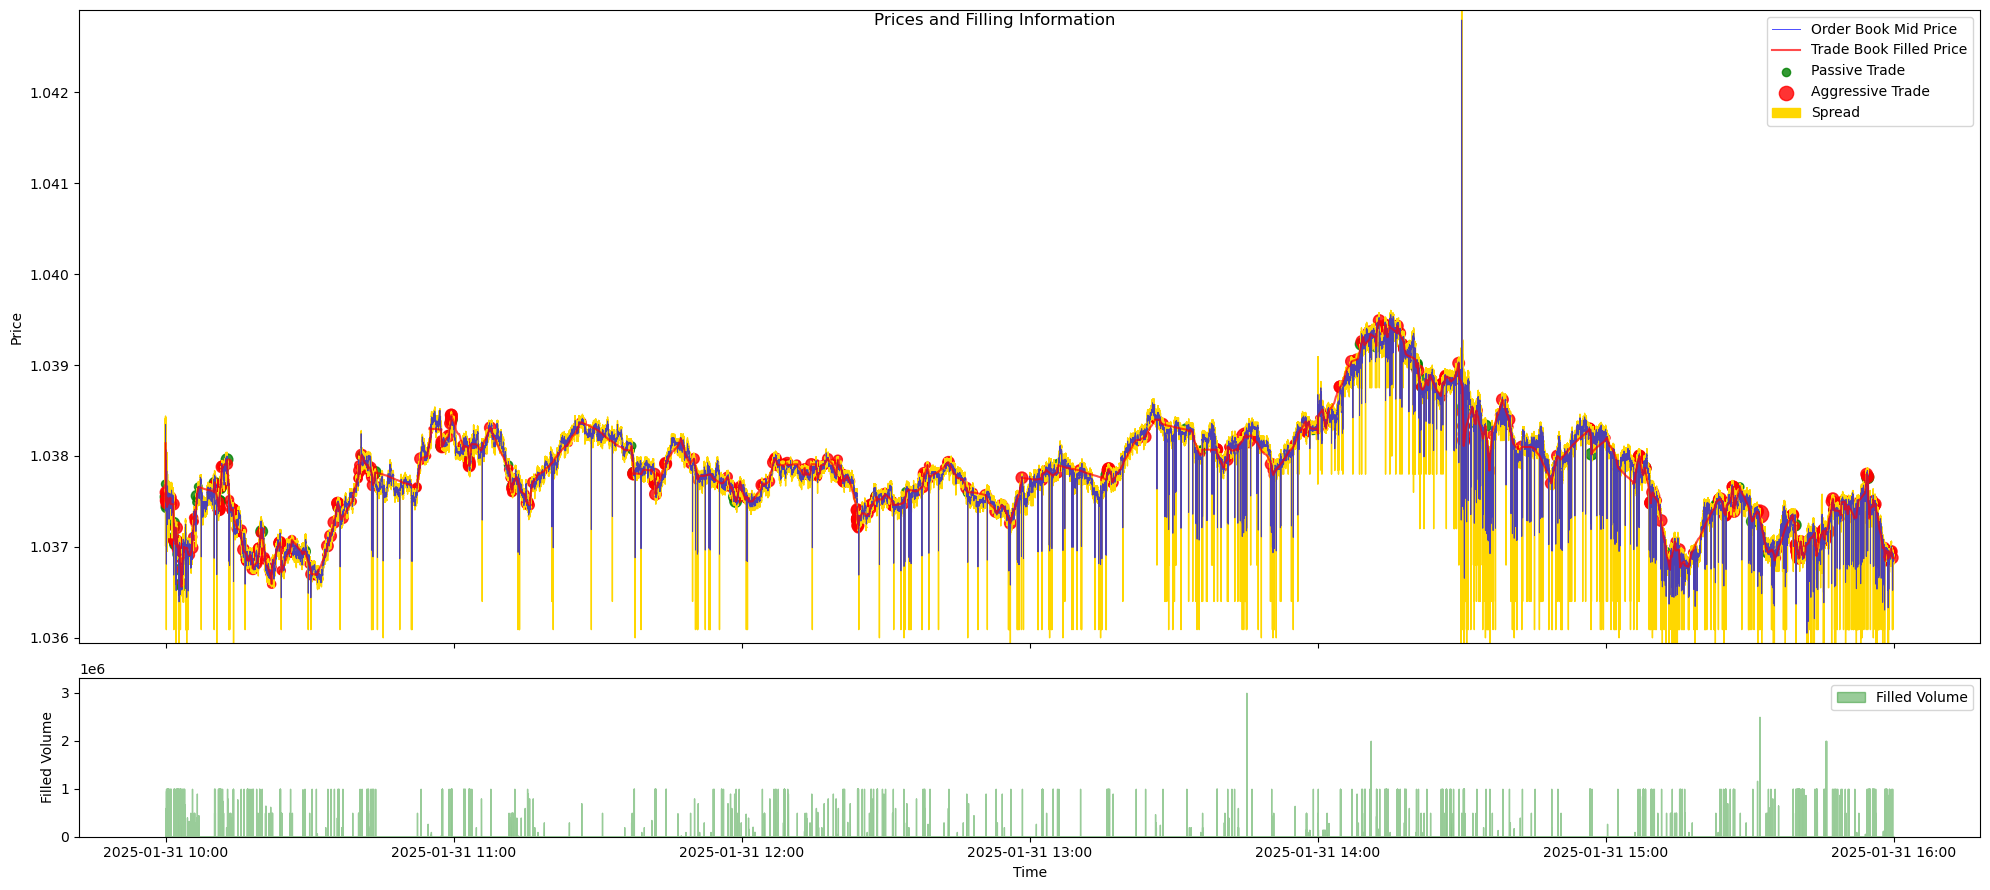
\includegraphics[width=1\linewidth]{figures/Prices and Filling Information.png}
%     \caption{Prices and filling information. This plot shows the mid-price from the order book (blue line), trade book filled prices (red line), and spread (yellow shading). Passive trades (green dots) and aggressive trades (red dots) are highlighted. The bottom panel represents the filled volume over time.}
%     \label{fig:p_f_i}
% \end{figure}


As can be seen in Figure~\ref{fig:p_f_i}, the mid-price has the highest point between 14:00 and 15:00. The filled price fits the mid-price well. I can see there are a lot of red dots which shows that they are aggressive trades. I did not classify bid or ask side because it's not the research target in the thesis. These aggressive trades go outside the spread range. The size of dots stands for relative volume of the trades. In other words, when the volume is large compared to other timestamps, the size of the dot will be larger. Therefore, I can easily see the active trading time point in the plot. Moreover, red dots represent aggressive trades in the trade book. I can see the red dots are more than green ones, which indicates that a lot of orders get filled by aggressive traders taking out them of the order book, instead of passively waiting for the market movements. This aligns with our need to improve the backtesting environment by predicting aggressive trades across the order book. Specially, there are several sparks in the trend of mid-price in the order book. Their frequent appearance in the plot suggests a systematic market behavior rather than random noise. These are caused by sudden jump in the best bid/ask price. As can be seen, most of them are downside sparks, which indicates that it seems the ask stays relatively stable while the bid collapses. This could be the reason that leads to sharp drops in mid-price.

From the bottom panel, in the beginning of 10:00, 15:45, 14:11, there are high volume up to 2,000,000, which are higher than common volume 1,000,000. At 13:45, the highest trading volume occurs as 3,000,000. Combined the two plots together, I can see when there's a drop, it's often accompanied by many trading records or large trades. 

In the Figure~\ref{fig:f_p_f_i} after filtering 2,381 sparks in the data, I can clearly see the price trends and some clustering for aggressive trades. For example, Table~\ref{tab:trade_sample} shows in the beginning of 10:00, many aggressive trades gather here. It may because there is a sharp dropping movement in the market, which triggers a wave of aggressive sell orders that consume the top levels of the bid side. This sudden removal of liquidity causes the mid-price to drop quickly, and encourages further aggressive selling or stop-loss execution.  

\begin{table}[htbp]
\centering
\caption{Sample of Trades and Order Book Information} 
\caption*{\textit{Note:} First 48 lines of the prices and filling information dataset, with 37 lines are hidden for simplification. Timestamps are in millisecond. $\bar{\alpha}$ indicates the trade is aggressive (1), passive (0) or no-trade (NaN). The hidden lines are all with NaN $\bar{\alpha}$. From the current data, several values of $\bar{\alpha}$ are 1 and only one is 0. This difference shows the importance of accurately predicting aggressive trades among all trade types. FPRICE and FVOLUME are filling prices and volumes respectively when trades happen. The spread and mid-price show volatility and variation over time. These patterns will be captured and used as features in the following sections.}
\small
    \begin{tabular}{l>{\raggedright\arraybackslash}p{3.3cm}cccccc}
    \toprule
    \textbf{Index} & \textbf{TIMESTAMP} & \textbf{$\bar{\alpha}$} & \textbf{FPRICE} & \textbf{FVOLUME} & \textbf{SPREAD} & \textbf{MID-PRICE} \\
    \midrule
    0  & 2025-01-31 10:00:00.007 & NaN & NaN   & 0.0      & 0.00042 & 1.037930 \\
    1  & 2025-01-31 10:00:00.012 & 1 & 1.038080 & 10000.0  & 0.00042 & 1.037930 \\
    2  & 2025-01-31 10:00:00.012 & 1 & 1.038140 & 1990000.0 & 0.00042 & 1.037930 \\
    3  & 2025-01-31 10:00:00.012 & 1 & 1.038140 & 10000.0  & 0.00042 & 1.037930 \\
    4  & 2025-01-31 10:00:00.017 & NaN & NaN & 0.0      & 0.00023 & 1.038325 \\
    5  & 2025-01-31 10:00:00.027 & NaN & NaN & 0.0      & 0.00007 & 1.038345 \\
    \vdots & \vdots & \vdots & \vdots & \vdots & \vdots & \vdots \\
    22 & 2025-01-31 10:00:00.195 & 1 & 1.037790 & 14841.0  & 0.00049 & 1.037745 \\
    23 & 2025-01-31 10:00:00.197 & NaN & NaN & 0.0      & 0.00054 & 1.037770 \\
    24 & 2025-01-31 10:00:00.205 & 1 & 1.037500 & 200000.0 & 0.00054 & 1.037770 \\
    25 & 2025-01-31 10:00:00.205 & 1 & 1.037500 & 180000.0 & 0.00054 & 1.037770 \\
    \vdots & \vdots & \vdots & \vdots & \vdots & \vdots & \vdots \\
    47 & 2025-01-31 10:00:00.417 & 0 & 1.037690 & 500000.0 & 0.00088 & 1.037980 \\
    % 48 & 2025-01-31 10:00:00.427 & NaN & 1.037680 & 0.0      & 0.00019 & 1.037635 \\
    % 49 & 2025-01-31 10:00:00.441 & NaN & 1.037670 & 0.0      & 0.00015 & 1.037615 \\
    \bottomrule
    \end{tabular}

\label{tab:trade_sample}
\end{table}


% \begin{sidewaysfigure}
%     \centering
%     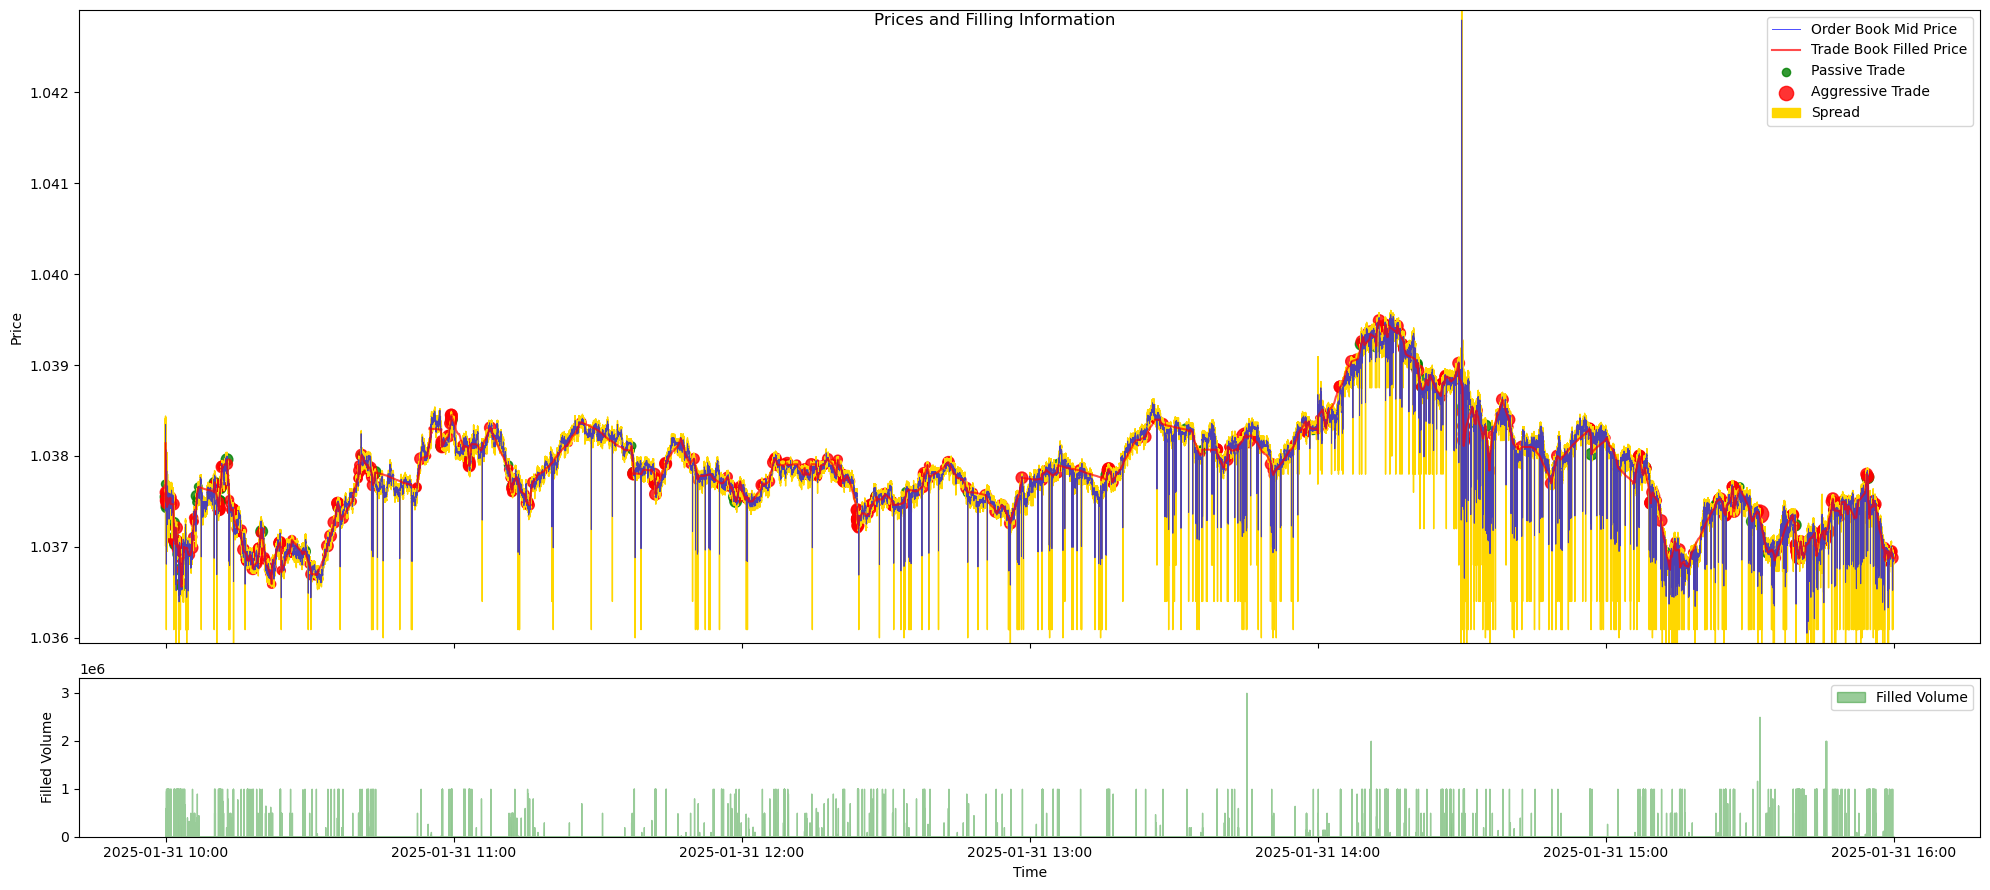
\includegraphics[width=\linewidth]{figures/Prices and Filling Information.png}
%     \caption{Prices and filling information}
%     \caption*{\textit{Note:} This plot shows the mid-price from the order book (blue line), trade book filled prices (red line), and spread (yellow shading). Passive trades (green dots) and aggressive trades (red dots) are highlighted. The bottom panel represents the filled volume over time.}
%     \label{fig:p_f_i}
% \end{sidewaysfigure}

% \begin{sidewaysfigure}
%     \centering
%     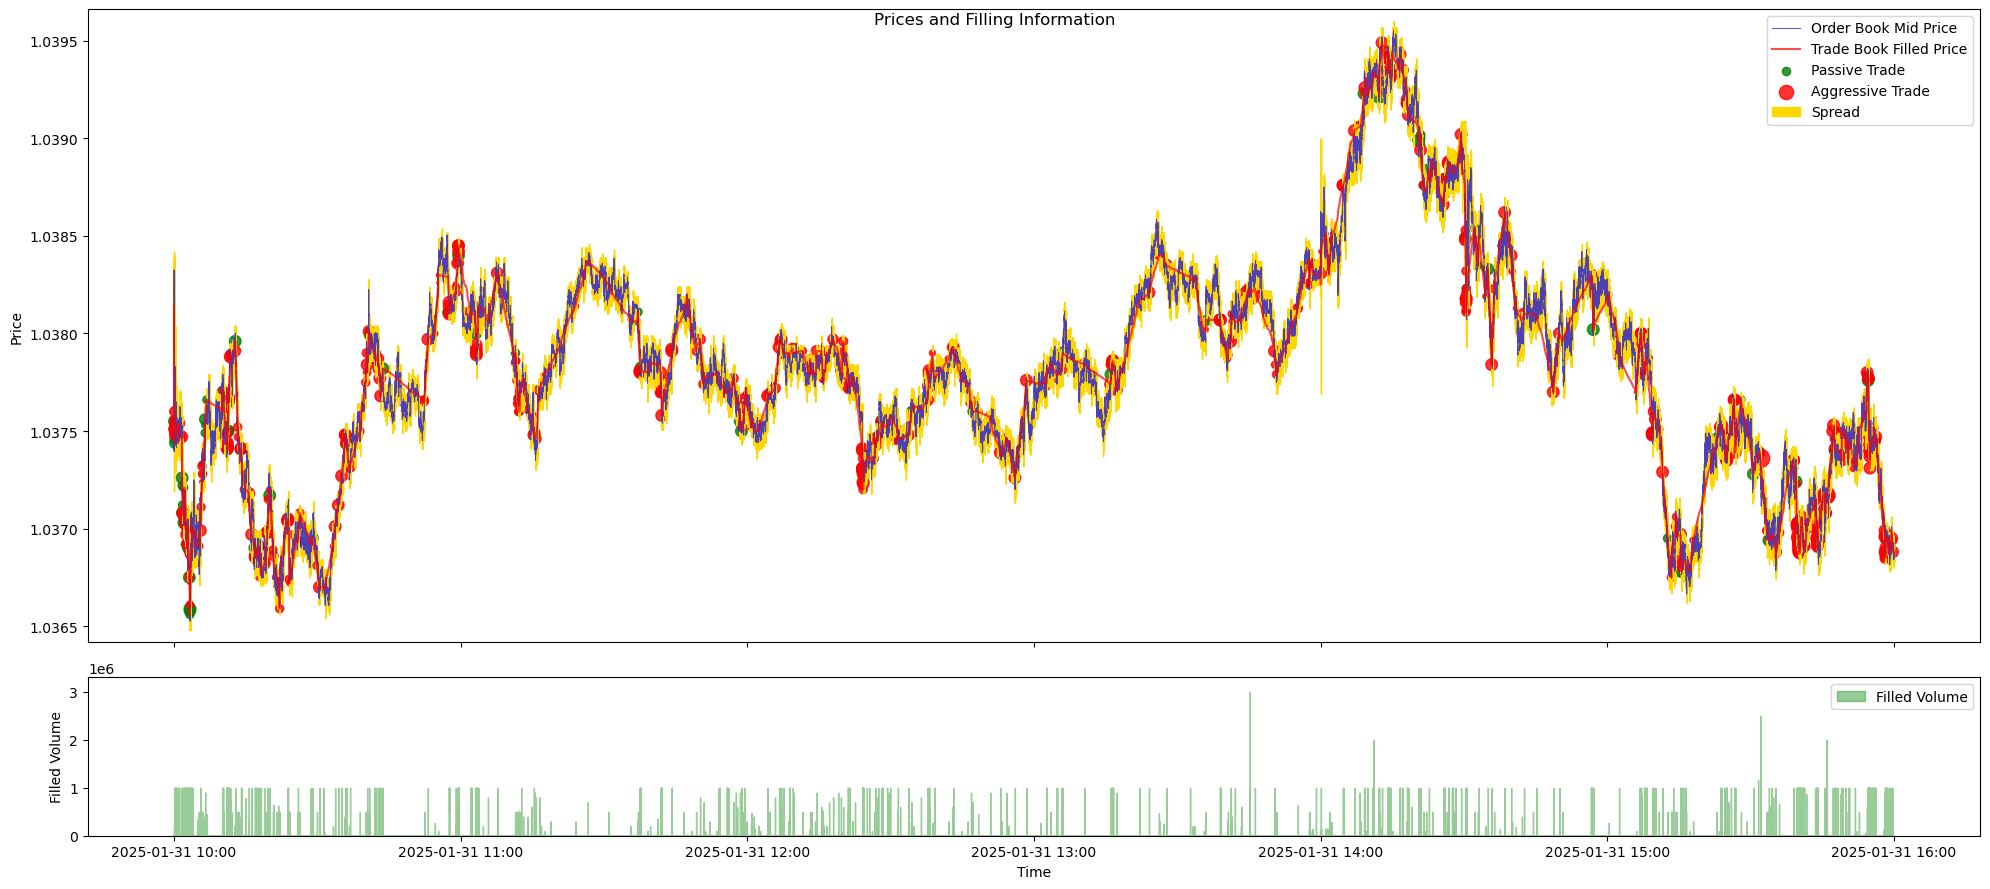
\includegraphics[width=\linewidth]{figures/Filtered Prices and Filling Information.png}
%     \caption{Filtered prices and filling information}
%     \caption*{\textit{Note:} Similar to Figure~\ref{fig:p_f_i}, but filtering sharp jump points. This plot shows the mid-price from the order book (blue line), trade book filled prices (red line), and spread (yellow shading). Passive trades (green dots) and aggressive trades (red dots) are highlighted. The bottom panel represents the filled volume over time. The price and trade dynamics remain the same.}
%     \label{fig:f_p_f_i}
% \end{sidewaysfigure}
\begin{figure}[p]
    \centering
    \rotatebox{90}{
        \begin{minipage}{\textheight}
            \centering
            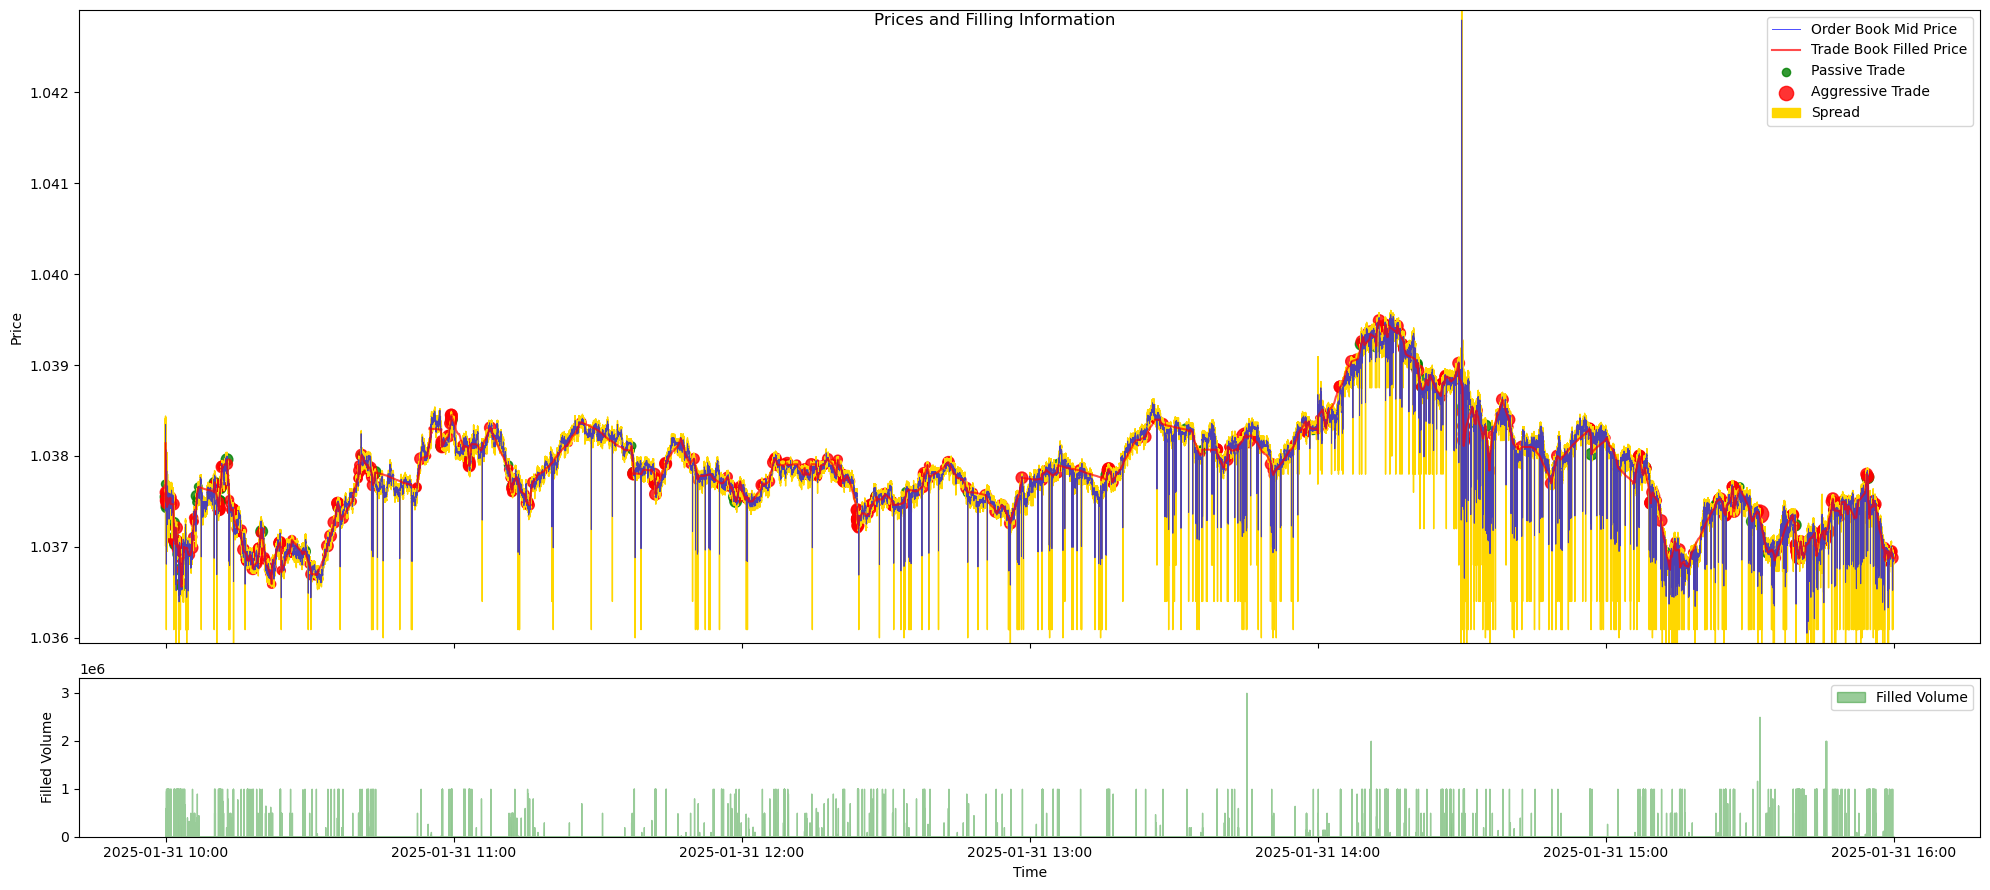
\includegraphics[width=\linewidth]{figures/Prices and Filling Information.png}
            \caption{Prices and filling information}
            \caption*{\textit{Note:} This plot shows the mid-price from the order book (blue line), trade book filled prices (red line), and spread (yellow shading). Passive trades (green dots) and aggressive trades (red dots) are highlighted. The bottom panel represents the filled volume over time.}
            \label{fig:p_f_i}
        \end{minipage}
    }
\end{figure}

\begin{figure}[p]
    \centering
    \rotatebox{90}{
        \begin{minipage}{\textheight}
            \centering
            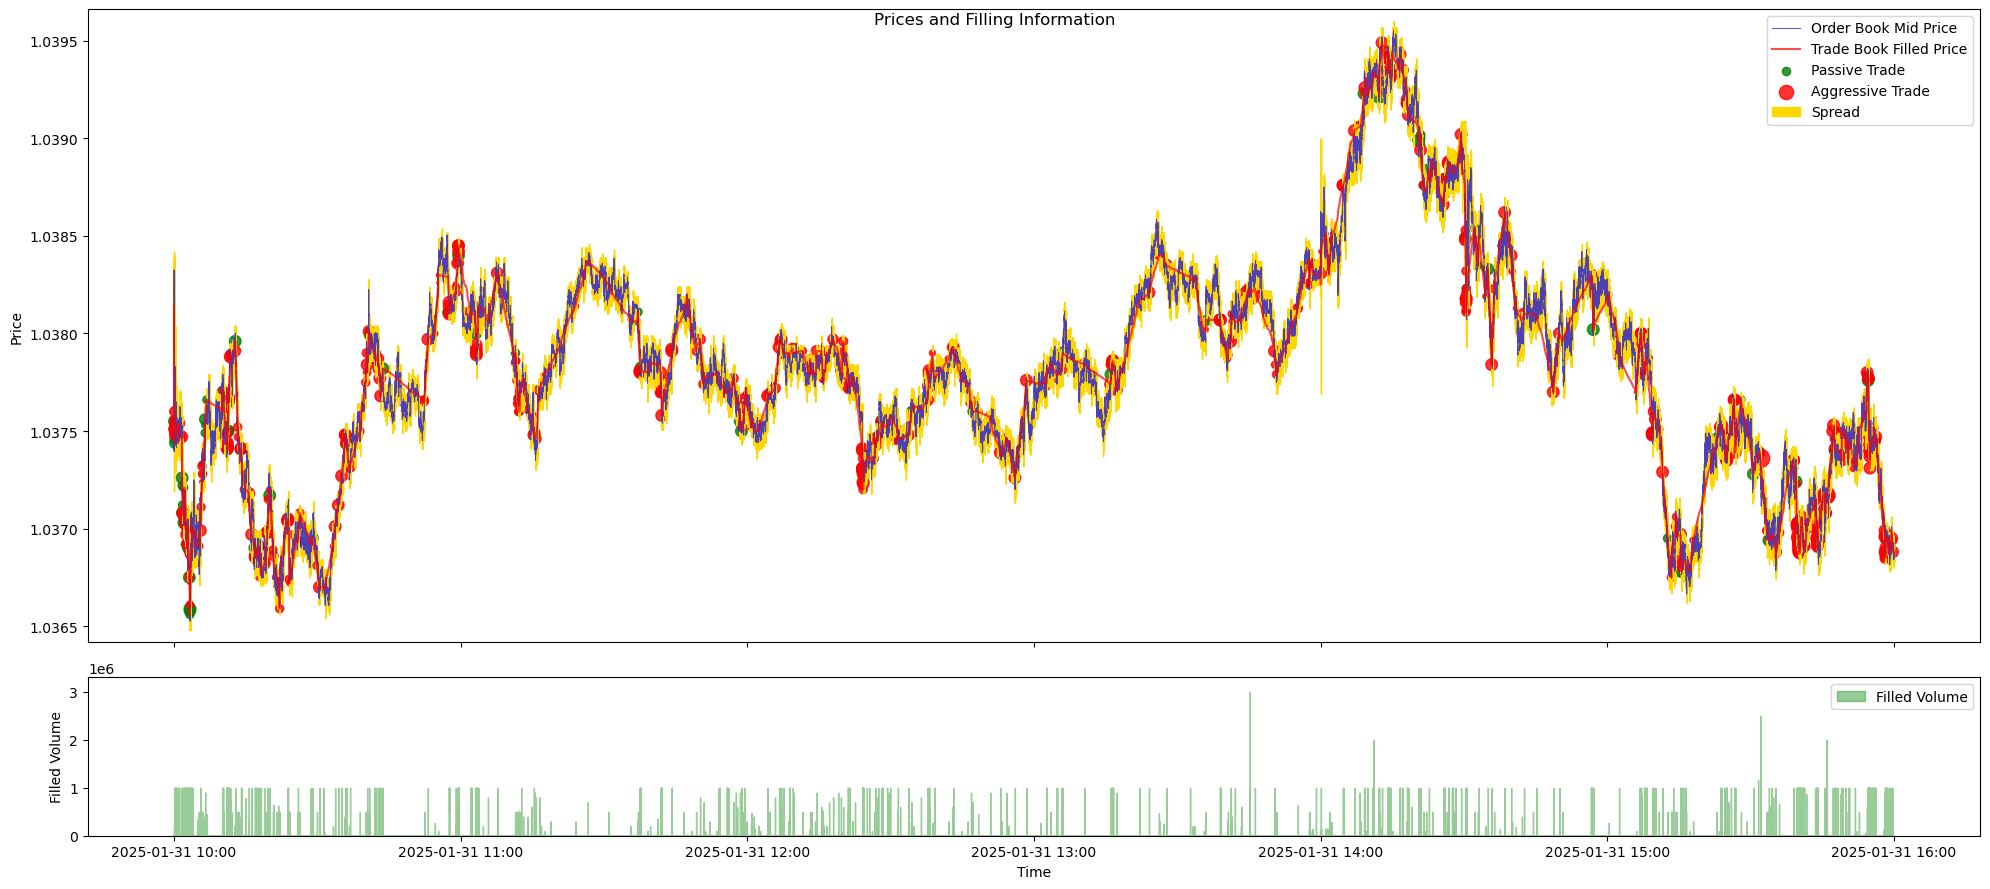
\includegraphics[width=\linewidth]{figures/Filtered Prices and Filling Information.png}
            \caption{Filtered prices and filling information}
            \caption*{\textit{Note:} Similar to Figure~\ref{fig:p_f_i}, but filtering sharp jump points. This plot shows the mid-price from the order book (blue line), trade book filled prices (red line), and spread (yellow shading). Passive trades (green dots) and aggressive trades (red dots) are highlighted. The bottom panel represents the filled volume over time. The price and trade dynamics remain the same.}
            \label{fig:f_p_f_i}
        \end{minipage}
    }
\end{figure}

\chapter{Methodology}\label{chapter:methodology}


% need change
This chapter discusses mathematical principles of models used in the thesis. The kernel metrics, basic dataset input for training, data processing methods and three prediction models are covered respectively, along with the intuition behind the methodology. In Section~\ref{sec:data-flow}, I summarize the whole data flow and how the three parts are connected. 

\section{Aggressive Trade: Target Variables}
In the FX trading market, once two orders get matched, the information is clearly recorded in trade book data, including the filling price, volume and direction where the order triggers. There are two ways of trading. Traders may aggressively participate and take out orders which are waiting in the order book. This happens when traders are eager to get trades done, putting more priority in time than price. Normally the filling price for this aggressive trade is higher (lower) than the mid-price and across the spread to touch even more aggressive price. In contrast to aggressive trade, it is also common that a trader just put forward a limit order and let it queue in the order flow. After positive market movements, the best bid/ask price matches the order price, the order is likely to get filled if it has the top priority. If the orders are matched, this information is also recorded in the trade book, but with a filling price at the best bid/ask. If it fails to match, it continues to stay in the order book and deepen the order book flow. Besides these two active trading situations, there are plenty of orders silently being submitted or staying and can not find any corresponding records in the trade book at the same timestamp. 

Two targets are provided in Section~\ref{sec: alpha} and Section~\ref{sec: aflag} which describe the trader behaviors in different situations. In the first section I introduce a continuous method to better understand the changing logic, while in the second section the real modeled target is shown and explained.

\subsection{Aggressiveness} \label{sec: alpha}
How aggressive a trader wants to submit orders and match existing orders is worth to discuss in this research. The purpose of defining it is to provide insight into aggressive trade behavior. It is not used in the model itself. In order to quantify and measure the level, I introduce a metric called \textit{aggressiveness}, denoted by $\alpha$:

\begin{equation}
    \alpha = \frac{P_F - P_B}{P_B}
    \label{eq: aggressiveness}
\end{equation}

$\alpha$ measures the aggressiveness of each trade. $P_F$ is the filling price at the time of the trade, and $P_B$ is the reference price used to determine whether a trade is aggressive. In this context, I set the benchmark as the previous mid-price in the order book, i.e., the mid-price from the most recent update before the current trade. For example, if a trader wants to buy and places an order above the mid-price to grab existing ask orders, this behavior is considered aggressive. The comparison is made against the last observed mid-price before the trader submitted the order. 

As shown in Equation~\ref{eq: aggressiveness}, for instance, on the bid side, $\alpha$ is positive if the filling price is higher than the benchmark price. This indicates that a trader is willing to buy at a price above the benchmark. Conversely, $\alpha$ is negative if the trader buys at a price below the benchmark. Similarly, on the ask side, $\alpha$ is negative when a trader sells at a price lower than the benchmark, and positive when the selling price exceeds the benchmark. Therefore, an aggressive trade is defined when $\alpha$ is positive on the bid side and negative on the ask side. When there are no trade records, $\alpha$ is assigned a value of 0. The meanings of different $\alpha$ values are summarized in Table~\ref{tb: alpha_meaning}. It is important to note that $\alpha$ is introduced only to help understand the aggressive trade situation and is not used in the modeling process. 

\begin{table}[h] 
    \centering 
    \begin{tabular}{lll} 
        \toprule 
        \textbf{$\alpha$} & \textbf{Meaning} & \textbf{Data Type} \\ 
        \midrule 
        $ > 0$ & Aggressive bid side trades, or passive ask side trades & Float \\
        $ < 0$ & Aggressive ask side trades, or passive bid side trades & Float \\ 
        $ = 0$ & No trades & Float \\  
        \bottomrule 
    \end{tabular} 
    \caption{Interpretation of $\alpha$ in Different Contexts}
    \label{tb: alpha_meaning}
\end{table}

\subsection{Binary Label for Aggressive Trade} \label{sec: aflag}
However, it is important to note that in the backtesting context at MN, I pay little attention to how aggressive a trader is, whether and when an aggressive trade will occur is more critical. Therefore, based on the $\alpha$, a binary target, called aggressiveness flag, denoted as $\bar{\alpha}$, is introduced. The direction of the trade is not considered by $\bar{\alpha}$ because I assume that traders will adjust order direction according to our order submission dynamically. $\bar{\alpha}$ is set to $0$ if no trade takes place or $\alpha$ is positive in ask side and negative in bid side takes at a given timestamp in the order book, and $1$ if $\alpha$ is possible in bid side and negative in ask side. 
\begin{table}[h] 
    \centering 
    \begin{tabular}{lll} 
        \toprule 
        \textbf{$\bar{\alpha}$} & \textbf{Meaning} & \textbf{Data Type} \\ 
        \midrule 
        $ = 1$ & Aggressive trades & Integer \\
        $ = 0$ & Both passive trades and cases where no trade occurred & Integer \\  
        \bottomrule 
    \end{tabular} 
    \caption{Interpretation of $\bar{\alpha}$ in Different Contexts}
    \label{tb: aflag_meaning}
\end{table}
In Table~\ref{tb: aflag_meaning}, I get binary flag $\bar{\alpha}$ which contains $1$ and $0$. It is reduced to a classification problem to solve by models, but the complexity of this issue comes from the class imbalance and feature dependencies. I will discuss them in the following contents in detail.



\section{Data Processing Methods}
% This part describes the dataset used for machine learning training, and resampling and rescale methods
The original order book data and trade book data (Table~\ref{tb: order book data description} and Table~\ref{tb: trade book data description}) fetched from Snowflake and exchange database are too raw to be modeled. In this section, I proceed to discuss methods that are used in data processing. First I discuss feature engineering. It is the process of transforming raw data into meaningful features that enhance the performance of machine learning models. I get effective features based on the calculation of spread, midprice and volume. Then another standard problem: class imbalance is analyzed.

Specifically, in Section~\ref{sec: training data}, I provide basic dataset for model training, test, estimation and prediction, along with specific formulas for certain features. The theoretical solution for extreme class imbalance is established in Section~\ref{sec: class imbalance}.

\subsection{Feature Engineering: Basic Dataset for Model Training} \label{sec: training data}
In selecting which features to generate, I inherit indicators from original order book and trade book, then extend them to get further features. The target discussed in Section~\ref{sec: aflag} is included as the basic dataset.

\begin{table}[h] 
    \centering 
    \begin{tabular}{lll} 
        \toprule 
        \textbf{Column} & \textbf{Description} & \textbf{Data Type} \\ 
        \midrule 
        $\bar{\alpha}$ & Binary flag & Integer \\
        $T$ & Timestamp of the snapshot in HH:MM.SSS & String \\
        \text{DIRECTION} & Bid($1$) or ask($-1$) trades & Integer \\
        $S$ & Difference between best ask and bid & Float \\
        $M$ & Middle price of best ask and bid & Float\\
        $V_A ^ {1}$ & Volume at best ask & Integer\\
        $V_B ^ {1}$ & Volume at best bid & Integer \\
        %$\alpha$ & How aggressive a trade is & Float \\ 
        %$\tau$ &  &  \\
        $\bar{\delta}_S$ & Average absolute spread change over the past 50 ticks & Float \\
        $\bar{\delta}_M$ & Average absolute mid-price change over the past 50 ticks & Float \\
        $\sigma_S$ & Volatility of spread over the last 50 ticks & Float \\
        $\sigma_M$ & Volatility of mid-price over the last 50 ticks & Float \\
        $r_V$ & Volume imbalance between best ask and bid & Float \\
        \bottomrule 
    \end{tabular} 
    \caption{Overall Dataset for Modeling}
    \label{tb: overall dataset for training}  
\end{table}
In the Table~\ref{tb: overall dataset for training}, capitalized terms refer to variables obtained directly from the order book and trade book data, including timestamp($T$), spread($S$), mid-price($M$), volume($V_A^{1}$, $V_B^{1}$). $T$ represents the time snapshot calculated relative to millisecond.

The last five features ($\bar{\delta}_S$, $\bar{\delta}_M$, $\sigma_S$, $\sigma_M$, $r_V$) are calculated from spread, mid-price or volume based on common factors which display order flow dynamics. $\bar{\delta}_S$ and $\bar{\delta}_M$ measure the local average absolute change over. They both capture the rapid changes in the cost of executing trades, directly related to liquidity changes in real market LOB dynamics. Specifically, $\bar{\delta}_M$ is useful to simulate realistic microstructure scenarios where aggressive trades tend to cluster, such as around price jumps. A 50-tick window is commonly used in high-frequency time series data because it effectively represents the local market environment without unnecessary noise or excessive smoothing. $\bar{\delta}_S$ and $\bar{\delta}_M$ can be formulated as follows:

\begin{equation}
    \bar{\delta}_{S_t} = \frac{1}{50} \sum_{i=0}^{49} \left| S_{t-i} - S_{t-i-1} \right| 
    \label{eq: spread change} 
\end{equation}
\begin{equation}
    \bar{\delta}_{M_t} = \frac{1}{50} \sum_{i=0}^{49} \left| M_{t-i} - M_{t-i-1} \right|
    \label{eq: midprice change} 
\end{equation}

Mid-price realized volatility affects order flows \citep{OrderAggressiveness2010}, thus $\sigma_M$ is used to depict the variability of mid-price changes. As defined in Equation~\ref{eq: midprice vola} and \ref{eq: spread vola}, standard deviation of mid-price changes and spread changes are calculated over a rolling window of 50 ticks. Spread factor $\sigma_S$ is also included because it reflects the consistency and variability of liquidity conditions.

\begin{equation}
    \sigma_{S_t} = \sqrt{\frac{1}{49}\sum_{i=0}^{48}\left((S_{t - i}-S_{t - i - 1})-\bar{\delta}_{S_t}\right)^2}
    \label{eq: spread vola}
\end{equation}

\begin{equation}
    \sigma_{M_t} = \sqrt{\frac{1}{49}\sum_{i=0}^{48}\left((M_{t - i}-M_{t - i - 1})-\bar{\delta}_{M_t}\right)^2}
    \label{eq: midprice vola}
\end{equation}

Higher $\bar{\delta}$ ($\bar{\delta}_S$ and $\bar{\delta}_M$) indicates that the market experiences frequent, sizable changes, with higher $\bar{\delta}_S$ reflecting unstable liquidity, and higher $\bar{\delta}_M$ showing active price discovery and increased market uncertainty. Conversely, lower $\bar{\delta}$ values signify stability, with lower $\bar{\delta}_S$ indicating consistent liquidity, and lower $\bar{\delta}_M$ suggesting calmer, more stable price movements.

Higher $\sigma$ ($\sigma_M$ and $\sigma_S$) represents greater variability and unpredictability in the market, with higher $\sigma_{S}$ highlighting liquidity risk, and higher $\sigma_{M}$ means significant fluctuations and uncertainty in the mid-price. Lower $\sigma$ denotes more predictable conditions, where lower $\sigma_{S}$ indicates stable liquidity conditions and lower $\sigma_{M}$ reflects reduced price uncertainty and market stability.

$r_V$ represents the relative imbalance between the ask and bid sides, as defined in Equation.~\ref{eq: volume ratio}. When $r_V$ approaches 1, most of the volume is concentrated on the ask side, indicating selling pressure in the limit order book. Conversely, when it approaches $-1$, the volume is mainly on the bid side, suggesting buying pressure. If $r_V$ is close to 0, the volumes are approximately balanced.
\begin{equation}
    r_V = \frac{V_A ^ {1} - V_B ^ {1}}{V_A ^ {1} + V_B ^ {1}}
    \label{eq: volume ratio}
\end{equation}

\subsection{Extreme Class Imbalance Solution} \label{sec: class imbalance}
% What is class imbalance
In a binary classification problem with data samples from two groups, class imbalance occurs when one class, the minority group, contains significantly fewer samples than the other class, the majority group \citep{johnson_survey_2019}. Extreme class imbalance refers to scenarios where the minority class represents less than 1\% of the total dataset \citep{leevy_survey_2018}. This level of imbalance brings significant challenges for machine learning algorithms, with strong bias results toward the majority class and may completely ignore the minority class in extreme cases. Extremely imbalanced datasets like this one are common in medicine and finance fields.

To predict aggressive trades in the limit order book, I study the aggressive trade flag ($\bar{\alpha}$). To demonstrate the imbalance clearly, one of a trading day is selected here, as shown in Figure.~\ref{fig: aflag_class_distribution}. $\bar{\alpha}$ faces severe class imbalance, which can lead to biased model predictions if not addressed. In the figure, class 0 dominates the dataset, accounting for 99.8\% of all samples, while Class 1 accounts for only 0.2\%. To solve this imbalance, techniques such as resampling, weighted loss function, and anomaly filter function are employed. 
\begin{figure}[h]
    \centering
    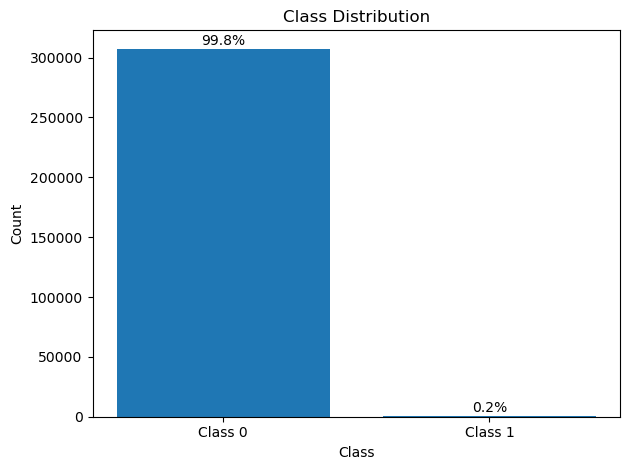
\includegraphics[width=0.8\linewidth]{figures/Imbalaced data for aflag.png}
    \caption{Class Distribution for $\bar{\alpha}$ on 31st January. In the overall 308,178 data, class 0 accounts for 99.8\% of the samples, while Class 1 represents only 0.2\%, indicating a severe class imbalance.}
    \label{fig: aflag_class_distribution}
\end{figure}

SMOTE (Synthetic Minority Over-sampling Technique) is an advanced oversampling method that generates synthetic samples of the minority class by interpolating between existing ones. However, since SMOTE connects both inliers and outliers arbitrarily, it may lead to a sub-optimal decision boundary, especially in high-dimensional and noisy datasets of our case. To better fit our dataset, I adopt a SMOTE variant called KMeansSMOTE, which applies KMeans clustering before performing oversampling. This clustering step groups similar samples together and generates synthetic data based on cluster density. For our high-frequency and extremely imbalanced data, KMeansSMOTE helps prevent synthetic samples from being generated in sparse or noisy regions, and creates more informative minority class samples that reflect the local data structure.
Let $\mathcal{X}_{\text{min}} = \{x_1, \dots, x_{N_{\text{min}}}\} \subset \mathbb{R}^d$ be the minority class. KMeansSMOTE proceeds as follows:

Apply KMeans to $\mathcal{X}_{\text{min}}$ with $k$ clusters:
  \[
  \min_{\{C_j\}} \sum_{j=1}^k \sum_{x \in C_j} \|x - \mu_j\|^2, \quad \mu_j = \frac{1}{|C_j|} \sum_{x \in C_j} x
  \]

For each cluster $C_j$, compute:
  \[
  \text{Density}_j = \frac{|C_j|}{\text{avg\_intra\_dist}(C_j)}, \quad w_j = \frac{1/\text{Density}_j}{\sum_{i} 1/\text{Density}_i}
  \]
where avg\_intra\_dist is the average pairwise distance within $C_j$. Set $n_j = \lfloor w_j \cdot n_{\text{gen}} \rfloor$.

For each $C_j$, repeat $n_j$ times:
  \[
  \tilde{x} = x + \lambda (x^{\text{NN}} - x), \quad \lambda \sim \mathcal{U}(0, 1)
  \]
where $x, x^{\text{NN}} \in C_j$ are randomly selected minority points and one of its $k$ nearest neighbors.

Building upon the foundation laid in the balanced class, weighted loss functions are implemented during the machine learning training process to focus on the accuracy of class 1. For example, in XGBoost, the weight is applied to the loss function by assigning a higher importance to the misclassification of class 1 samples. Specifically, the objective function includes a weighted logistic loss where the weight $w_i$ for each instance increases if the sample belongs to the target class, influencing both the gradient and Hessian in the boosting process. Additionally, take GRU-based RNN for another example, class weights are introduced in the binary cross-entropy loss function. The loss becomes:
\[
\mathcal{L} = -w_1 \cdot y \cdot \log(\hat{y}) - w_0 \cdot (1 - y) \cdot \log(1 - \hat{y})
\]
where $w_1$ and $w_0$ are the weights for class 1 and class 0, respectively, $y$ is the true label, and $\hat{y}$ is the predicted probability. This weighted loss penalizes the model more for errors on class 1, guiding it to pay more attention to the target class during training.

Anomaly filter methods are also applied to highlight the regions around aggressive trading events. This thesis presents a window-based filter function to extract time segments centered around class 1 instances. Specifically, for each sample with a non-missing DIRECTION label, which means there is at least one trade recorded, a window of certain milliseconds is defined. All entries within this time range are included for training. This method ensures that the model is exposed to a richer context around potential anomalies and enhances the learning of class 1 patterns in the high-frequency setting. In our practical implementation, I integrate an anomaly detection function alongside KMeansSMOTE across different models. This ensures that imbalanced class problem are handled without conflict in each model and maintains balanced class distributions consistently between the models.

\begin{algorithm}[H]
\caption{Window-Based Anomaly Filter} \label{al: window-based}
\begin{algorithmic}[1]
\State \textbf{Input:} Data with timestamps and labels; window size $\delta$
\State \textbf{Output:} Filtered data around class 1 instances
\For{each timestamp $t$ where \texttt{DIRECTION} is not NaN}
    \State Define window: $[t - \delta/2,\ t + \delta/2]$
    \State Find all rows within this window and add their indices to \texttt{result\_indices}
\EndFor
\State \Return rows corresponding to \texttt{result\_indices}
\end{algorithmic}
\end{algorithm}


\section{Prediction Model: An XGBoost-Enhanced Neural Hawkes Process Framework}
This thesis proposes an XGBoost-enhanced Neural Hawkes Process framework combining class imbalance solutions, neural encoder, and stochastic modeling to predict aggressive trades under extreme class imbalance. The framework is designed to first resolve class imbalance through resampling in XGBoost, then integrate nonlinear and long-range feature dependencies, which are extracted from recurrent neural networks, into the calculation of intensity in Hawkes processes. 

To depict the general workflow of our framework, Figure~\ref{fig:data-flow-diagram} presents the overall workflow of our framework, combining both the training (estimation) phase and the testing phase. More detailed and clearly separated diagrams will be discussed in Section~\ref{sec:data-flow}. The framework begins with an XGBoost classifier trained to identify aggressive trade events from limit order book features displayed in Table~\ref{tb: overall dataset for training}. 

To address the extreme class imbalance in the dataset, KMeansSMOTE is applied during training to generate synthetic minority samples in a structure-aware manner, ensuring a more balanced and representative training set. The first-filtered output of the XGBoost model, alongside features, is then fed into a Gated Recurrent Unit (GRU), which acts as a historical market state encoder. The GRU transforms the inputs into a compact hidden state that captures nonlinear dependencies and long-range dynamics in condition of temporal logic ($T$) and market features ($S$, $M$, $V_A^{1}$, $V_A^{1}$, $\bar{\delta}_S$, $\bar{\delta}_M$, $\sigma_S$, $\sigma_M$, $r_V$). This hidden state is used to condition the intensity function $\lambda(t)$ of a neural Hawkes process. Unlike classical Hawkes models based on additive exponential kernels, the intensity here is dynamically modulated by the GRU output, allowing the model to flexibly capture evolving market microstructure behavior. As a result, the process becomes a conditional point process, where the estimation of parameters is informed by both structured and balanced output of the XGBoost model and the latent dynamics embedded in recent order book activity.

In the first stage, I employ XGBoost to predict $\bar{\alpha}$ on the full trading day using limit order book features in Table~\ref{tb: overall dataset for training}. To address the extreme class imbalance and get potential aggressive trade rows, I apply KMeansSMOTE before training. This first classifier aims to identify as many true trade points as possible (high recall) and increase the proportion of minor class in the output. The model filters out most of the non-aggressive instances (class 0) and provides a broad set of aggressive trade activity candidates. This output serves two purposes: it reduces the candidate space for aggressive trade prediction, and its feature importance guides the selection of input features for subsequent models.

In the second stage, I train a GRU-based recurrent neural network to get the hidden state formula of the two market scenarios as mentioned in Table~\ref{tb: aflag_meaning} (aggressive and non-aggressive). The GRU model is trained on a balanced dataset constructed using a window-based anomaly filter function around class 1 labels as presented in Algorithm~\ref{al: window-based}. This stage further refines the prediction of aggressive trades by deep learning networks. The GRU hidden state captures these invisible market conditions that traditional Hawkes can not see, but that critically affect event intensity.

In the final stage, I apply a neural Hawkes process to analyze a more dynamic estimation and prediction of aggressive trades. The Hawkes model captures the temporal clustering of aggressive trade events and demonstrates interpretable output in the form of aggressive and non-aggressive trade intensity and probability. This significantly compensates for the limited ability of machine learning models. I also incorporate a condition based on MN trade execution information: if an internal order is filled within certain milliseconds window, it increases the likelihood of a nearby aggressive trade. This step not only enhances the final accuracy and F1 score, but also produces a more interpretable, precise and inclusive prediction set.

Overall, this framework effectively predicts rare aggressive trades by combining class imbalance solution, market states features, temporal dependency, and clustering modeling. It predicts the intensity and final pattern of aggressive and non-aggressive events. The following parts of the section elaborate each of the three components and discuss the combined contribution of the predictive framework.

\begin{figure}[H]
    \centering
    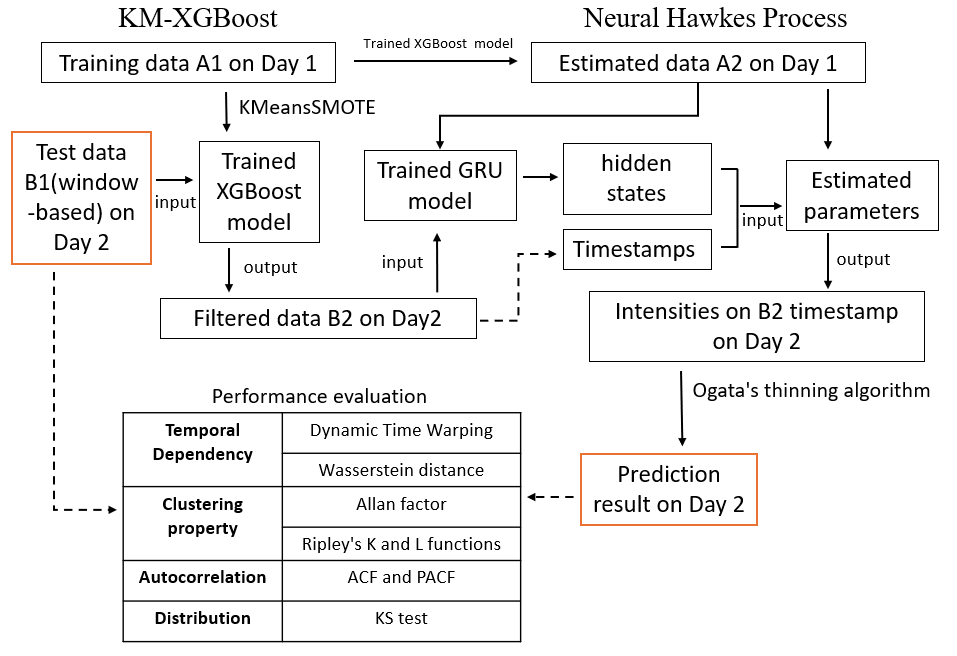
\includegraphics[width=0.8\textwidth]{figures/data_flow1.png}
    \caption{Data flow of the full pipeline from raw data to final prediction, combining both training and testing stages.}
    \label{fig:data-flow-diagram}
\end{figure}


\subsection{XGBoost with KMeansSMOTE Filtering (KM-XGBoost)}
XGBoost is a tree-based ensemble learning method that builds a sequence of decision trees to minimize a specified loss function. With a gradient boosting logic, each new tree is trained on the residual errors of the current model, effectively correcting its mistakes by following the negative gradient of the loss. 

XGBoost is a strong overall model, which includes features that make it especially practical and powerful in real-world applications. \cite{XGBoost_2016} compare XGBoost with some other popular classifiers, and find XGBoost helps prevent overfitting through built-in regularization, can handle sparse data automatically without preprocessing, and is optimized for speed and memory efficiency, making it well-suited for large-scale datasets with imbalanced data. XGBoost can capture nonlinear patterns that logistic regression cannot, and handles sparse data with native sparsity-aware algorithms. Compared to GBM (Traditional Gradient Boosting Machines), XGBoost significantly outperforms them in training time (up to 10x faster) and often in test accuracy. In the context of Kaggle competitions, XGBoost outperforms neural networks, especially in tabular data, and top entries use XGBoost rather than deep learning models \citep{XGBoost_2016}. It represents that XGBoost is easier to tune and more robust to hyperparameter choices in those settings and less data-hungry than deep neural nets.

The underlying objective function of XGBoost can be explained as follows: a loss term and a regularization term. It is defined as:

\begin{equation}
\mathcal{L}(\phi) = \sum_{i=1}^{n} l(y_i, \hat{y}_i^{(t)}) + \sum_{k=1}^{t} \Omega(f_k)
\end{equation}

Where $l$ is a differentiable convex loss function, such as the logistic loss for binary classification. It measures the difference between the true label $y_i$ and the predicted value $\hat{y}_i^{(t)}$ at iteration $t$. The second term, $\Omega(f_k)$, is a regularization function that penalizes the complexity of each added tree $f_k$.

The regularization term is defined as:

\begin{equation}
\Omega(f) = \gamma T + \frac{1}{2} \lambda \|w\|^2
\end{equation}

Here, $T$ denotes the number of leaves in the regression tree, $w$ represents the vector of scores assigned to the leaves, and $\gamma$, $\lambda$ are regularization parameters that control the penalty on the number of leaves and the magnitude of leaf weights respectively. If $T$ is larger, it gives better data fitting and gets penalties by $\lambda$ and $\lambda \|w\|^2$, avoiding overfitting.

This thesis uses GridSearchCV and cross-validation to find the best hyperparameters for the XGBoost model. GridSearchCV is a module from the Python library scikit-learn \citep{scikit-learn2011}, which performs an ergodic search over a grid of hyperparameter values. It combines this with cross-validation, a technique that splits the training data into multiple folds. In each round, one fold is used for validation and the others for training. This helps to evaluate the model performance more fairly and avoids overfitting to one specific subset of data. 

Algorithm~\ref{alg: grid_search} demonstrates the setup of hyperparameter tuning. The search is conducted over three values each for $n\_estimators$ (number of boosting rounds), $max\_depth$, $learning\_rate$, and $min\_child\_weight$. One fixed value of $scale\_pos\_weight$, which was computed based on the class imbalance ratio. The evaluation metric used is ROC-AUC, which is especially suitable for imbalanced classification tasks. A 3-fold cross-validation ($cv=3$) is applied, and the search is performed in parallel using all available CPU cores ($n\_jobs=-1$) for efficiency. To give more focus on aggressive trades, instance weights are manually adjusted before fitting: class 1 (aggressive trades) is assigned a higher weight (100.0), while class 0 (non-aggressive trades) receives a weight of 1. This weighting helps the model pay more attention to aggressive trades during training.

% \begin{algorithm}[H]
% \caption{Grid Search with Cross-Validation for XGBoost} \label{alg: grid_search}
% \begin{algorithmic}[1]
%     \State Define base XGBoost model with fixed settings:
%     \Statex \hspace{\algorithmicindent} \texttt{use\_label\_encoder=False}, \texttt{eval\_metric='logloss'}, \texttt{random\_state=42}
%     \State Define hyperparameter grid:
%     \Statex \hspace{\algorithmicindent} \texttt{n\_estimators} $\in \{100, 300, 500\}$
%     \Statex \hspace{\algorithmicindent} \texttt{max\_depth} $\in \{3, 5, 7\}$
%     \Statex \hspace{\algorithmicindent} \texttt{learning\_rate} $\in \{0.01, 0.02, 0.05\}$
%     \Statex \hspace{\algorithmicindent} \texttt{min\_child\_weight} $\in \{3, 5, 7\}$
%     \Statex \hspace{\algorithmicindent} \texttt{scale\_pos\_weight} = computed class imbalance ratio
%     \State Initialize GridSearchCV with:
%     \Statex \hspace{\algorithmicindent} scoring metric: ROC-AUC
%     \Statex \hspace{\algorithmicindent} cross-validation folds: 3
%     \Statex \hspace{\algorithmicindent} parallel jobs: all CPUs (\texttt{n\_jobs=-1})
%     \State Compute sample weights:
%     \Statex \hspace{\algorithmicindent} weight = 100.0 for aggressive trades
%     \Statex \hspace{\algorithmicindent} weight = 1.0 for non-aggressive trades
%     \State Fit model to resampled training data using \texttt{sample\_weight}
%     \State Return best hyperparameters and cross-validated model
% \end{algorithmic}
% \end{algorithm}

\begin{algorithm}[H]
\caption{Grid Search with Cross-Validation for XGBoost}\label{alg: grid_search}
\begin{algorithmic}[1]
    \State Define base XGBoost model:
    \Statex \hspace{\algorithmicindent} \texttt{use\_label\_encoder=False}, \texttt{eval\_metric='logloss'}, \texttt{random\_state=42}
    \State Define base XGBoost model with fixed settings:
    \Statex \hspace{\algorithmicindent} \texttt{use\_label\_encoder=False}, \texttt{eval\_metric='logloss'}, \texttt{random\_state=42}
    \State Define hyperparameter grid:
    \Statex \hspace{\algorithmicindent} \texttt{n\_estimators} $\in \{100, 300, 500\}$
    \Statex \hspace{\algorithmicindent} \texttt{max\_depth} $\in \{3, 5, 7\}$
    \Statex \hspace{\algorithmicindent} \texttt{learning\_rate} $\in \{0.01, 0.02, 0.05\}$
    \Statex \hspace{\algorithmicindent} \texttt{min\_child\_weight} $\in \{3, 5, 7\}$
    \Statex \hspace{\algorithmicindent} \texttt{scale\_pos\_weight} = computed class imbalance ratio
    \State Initialize GridSearchCV with:
    \Statex \hspace{\algorithmicindent} scoring metric: ROC-AUC
    \Statex \hspace{\algorithmicindent} parallel jobs: all CPUs (\texttt{n\_jobs=-1})
    \State Compute sample weights:
    \Statex \hspace{\algorithmicindent} weight = 100.0 for aggressive trades
    \Statex \hspace{\algorithmicindent} weight = 1.0 for non-aggressive trades
    \ForAll {hyperparameter combinations in grid}
        \For{fold $k = 1$ to $K$ (e.g. 3)}
            \State Split data into training set $D_{\text{train}}^{(k)}$ and validation set $D_{\text{val}}^{(k)}$
            \State Train model on $D_{\text{train}}^{(k)}$ using sample weights
            \State Evaluate ROC-AUC on $D_{\text{val}}^{(k)}$
        \EndFor
        \State Compute average ROC-AUC across $K$ folds
    \EndFor
    \State Select the hyperparameter set with the highest average ROC-AUC
    \State Re-train final model on full training set using selected hyperparameters
\end{algorithmic}
\end{algorithm}

The architecture of XGBoost encourages the model to fit the data effectively with awareness of class focus, while avoiding overfitting by controlling model complexity. This results in a faster and more practical training process.

In our study, KMeansSMOTE is applied to the training data to address class imbalance before feeding it into XGBoost. XGBoost is then used to predict $\bar{\alpha}$ and to generate feature importance scores. These scores serve as a reference for selecting relevant features in the subsequent neural network training. This feature selection step helps reduce model complexity and focuses the learning process on the most informative patterns. The input-output workflow of this process can be summarized as follows:
\begin{itemize}
  \item \textbf{Input:}  
  The model receives a resampled dataset obtained by applying KMeansSMOTE to the original data presented in Table~\ref{tb: overall dataset for training}. The resampling adjusts the class distribution to approximately 3:7 (aggressive:non-aggressive). Input features include engineered features $S$, $M$, $V_A^{1}$, $V_A^{1}$, $\bar{\delta}_S$, $\bar{\delta}_M$, $\sigma_S$, $\sigma_M$, $r_V$.

  \item \textbf{Model Configuration:}  
  An XGBoost classifier is trained using hyperparameters selected via GridSearchCV. The final model configuration is:
  \begin{itemize}
    \item \texttt{n\_estimators} = 500
    \item \texttt{max\_depth} = 7
    \item \texttt{min\_child\_weight} = 5
    \item \texttt{learning\_rate} = 0.05
    \item \texttt{scale\_pos\_weight} = computed imbalance ratio
    \item \texttt{eval\_metric} = 'logloss'
    %\item \texttt{random\_state} = 42
  \end{itemize}

  \item \textbf{Output:}  
  The model outputs a binary prediction for each record in the time window of a given trading day, indicating whether the event is likely to be an aggressive trade (\texttt{class = 1}). The output gives a more balanced class dataset, with the class 1 (aggressive trade) accounting for approximately 10\% of the whole data.

\end{itemize}



%-------------------------GRU-----------------------------
\subsection{Gated Recurrent Units (GRU)-based RNN}
% what's GRU
To model the nonlinear and long-range sequential dynamics in condition of market features of aggressive trades, I employ a recurrent neural network (RNN) based on GRU. GRU is a type of neural network designed to work with sequential data alongside engineered features, such as time series, sentences, or trading records. Unlike standard models that treat each input independently, a GRU learns from past information and current input at the same time. When I deal with data that unfolds over time, like a series of trades, it's important to understand how earlier events influence later ones. For example, an aggressive trade might be more likely to happen now if the spread was very low several ticks ago. 

% why GRU not others
GRU is a simplified variant of the Long Short-Term Memory (LSTM) network, designed to capture long-range dependencies while using fewer parameters and computational resources \citep{GRU2014}. It has a simplified architecture with two gates: the update gate and reset gate. The update gate controls how much of the previous hidden state should be retained, and the reset gate determines how much of the past information to forget. The two gates allow the model to remember or forget past information as needed, crucial for understanding market patterns in order book data. Since it lacks the forget gate, compared to LSTM, GRU has fewer parameters and faster training times, making it more efficient for larger datasets. In many cases, the performance difference between LSTM and GRU is not significant, and GRU is often preferred due to its simplicity and efficiency. 

In our study, I adopt a GRU architecture instead of the LSTM structure used by \cite{lalor_event-based_2025} because our problem involves fewer event types, but much higher frequent dynamics, where fast and robust convergence is critical. More specifically, Table~\ref{tab:gru_vs_lstm} compares the use of GRU with the LSTM approach used by \cite{lalor_event-based_2025}.

\begin{table}[H]
\centering
\caption{Comparison of LSTM-Based Model vs. GRU-Based Model}
\begin{tabular}{p{3cm} p{5.5cm} p{5.5cm}}
\toprule
\textbf{Aspect} & \textbf{LSTM-Based Model} & \textbf{GRU-Based Model} \\
\midrule
\textbf{Data Domain} & Stock LOBSTER data (lower tick frequency, long time span) & FX spot market data (millisecond frequency, short time window) \\
\textbf{Purpose} & Simulates all 12 LOB event types & Predicts binary outcome \\
\textbf{Complexity} & High: expressive but computationally intensive & Low: efficient and sufficient for task-specific modeling \\
\textbf{Training Time} & Slower convergence; more resource intensive & Faster training; lightweight structure \\
\textbf{Overfitting Risk} & High: due to model size and variable performance across assets & Lower: binary setting with consistent performance \\
\bottomrule
\end{tabular}
\label{tab:gru_vs_lstm}
\end{table}

On the one hand, the LSTM-based approach is designed to handle a large and diverse set of 12 LOB event types. This level of event complexity and inter-type interaction needs a more complicated but also heavier architecture like LSTM. In contrast, our setting focuses on a simpler and more specific prediction task. Our training dataset contains just two types of market scenarios (aggressive vs. non-aggressive trades). I do not simulate all LOB events but instead focus on binary classification. Therefore, the computational burden of LSTM is unnecessary, and the more efficient GRU offers a faster and equally expressive alternative for our goal.

On the other hand, \cite{lalor_event-based_2025} relied on stock data from LOBSTER. It is relatively lower tick frequencies compared to higher-frequent FX spot markets. As a result, fast and robust convergence is critical. GRU is a more suitable RNN to predict aggressive trade pattern in the high frequency FX spot market.


% why hidden states matter and math formulas
GRU helps the model remember those earlier patterns by giving a hidden state. It is a memory storage that is updated at each step in the sequence. The core assumption behind using an RNN is that the current output depends not only on the current input but also on the historical sequence of past inputs. Formally, a GRU updates its hidden state through gating mechanisms that regulate the flow of information, allowing it to selectively retain or forget past information as needed. It can consist of multiple stacked GRU layers and be followed by a dense output layer. Each GRU layer returns sequences to preserve the full temporal structure across time steps. The model is trained to minimize a weighted mean squared error (MSE) loss. 
\begin{equation}
    \mathcal{L} = \frac{1}{N} \sum_{i=1}^{N} \sum_{t=\text{warmup\_steps}}^{T} w_{i,t} \left( y_{i,t} - \hat{y}_{i,t} \right)^2
    \label{eq:GRU loss function}
\end{equation}
    where
\begin{equation}
    w_{i,t} =
    \begin{cases}
    w_\text{nozero}, & \text{if } y_{i,t} \neq 0 \\
    w_\text{zero}, & \text{if } y_{i,t} = 0
    \end{cases}
    \label{eq:weight in GRU loss}
\end{equation}
    
In Equation.~\ref{eq:GRU loss function} and \ref{eq:weight in GRU loss}, higher importance is given to nonzero targets to emphasize the prediction of aggressive behaviors. Furthermore, the initial warmup steps are ignored in each sequence when calculating the loss. During this phase, hidden state representations are still developing, and their predictions are often noisy \citep{lambrechts2023warmingrecurrentneuralnetworks}. This can prevent the model from being penalized during its early and uncertain predictions.

The GRU works through four simple steps. First, the reset gate $r_t$ decides how much of the previous memory to forget when creating new information. If values close to 0, it forgets most of the past and values, while values closing to 1 mean remember everything. Next, the update gate $z_t$ acts as a mixing controller that determines how much to blend old memory with new information. The candidate hidden state $\tilde{h}_t$ represents the proposed new memory based on the current input. Finally, the most important part, actual hidden state $h_t$, is computed as a weighted average between the old memory and the new candidate. It controls how much of the old memory should be used to create new information, and how much should the memory be updated with this new information.
\begin{align}
    % Reset Gate
    r_t = \sigma(W_r \cdot [h_{t-1}, x_t] + b_r) \\
    % Update Gate
    z_t = \sigma(W_z \cdot [h_{t-1}, x_t] + b_z) \\
    % Candidate Hidden State
    \tilde{h}_t = \tanh(W_h \cdot [r_t \odot h_{t-1}, x_t] + b_h) \\
    % Final Hidden State
    h_t = (1 - z_t) \odot h_{t-1} + z_t \odot \tilde{h}_t
\end{align}

% input and output
In our study, the model is trained to capture hidden states which can keep useful memory of past inputs. These hidden states are later used as dynamic inputs for the Hawkes process. It works well enough for our binary trade prediction task and helps connect market features with intensity estimation. The input-output workflow of this process can be summarized as follows:

\begin{itemize}
  \item \textbf{Input:}  
  An anomaly filter is applied to the raw dataset. For each record with a valid \texttt{DIRECTION} label, a fixed-width time window is constructed. All entries falling within this window are collected to form a training sample. This ensures the filtered dataset maintains approximately 10\% aggressive trades, aligning with the XGBoost classifier's output distribution.

  Before training, features and labels are scaled using \texttt{MinMaxScaler()}, and sequences are reshaped with a fixed length of 3000 time steps. The training is conducted using a batch size of 32.

  \item \textbf{Model Configuration:}  
  A GRU-based model is defined using Keras \texttt{Sequential()}:
  \begin{itemize}
    \item First layer: GRU with 1024 units, returning sequences.
    \item Second layer: Fully connected \texttt{Dense} layer with sigmoid activation.
    \item Optimizer: RMSprop with learning rate $10^{-3}$
    \item Loss function: custom \texttt{loss\_mse\_warmup} to exclude initial warmup steps from the loss.
  \end{itemize}

  The model is trained with \texttt{model.fit()} using a generator that yields sequences, over 6 epochs with 6 steps per epoch. These settings are selected based on convergence behavior.

  \item \textbf{Output:}  
  After training, a hidden state extraction function is applied to retrieve the dynamic GRU hidden states at each timestamp for both aggressive (class 1) and non-aggressive (class 0) trades. These hidden states are then used to condition the intensity function in the subsequent Hawkes process.
\end{itemize}




\subsection{Neural Hawkes Process}
% what is Hawkes and how our neural HP nice
The Hawkes process is a self-exciting point process that models events happening over time. It is called 'self-exciting' because each event can make future events more likely (or less likely) to happen soon after. This is different from normal classification models that give a yes-or-no answer. The Hawkes process gives a time-varying intensity function, written as $\lambda(t)$, which represents the conditional probability density of the occurrence of an event in the immediate future \citep{bacry_hawkes_2015}. 

I use a neural Hawkes process to improve this traditional model. Instead of using fixed formulas, I let a neural network reinforce the calculation of the intensity function. This makes the model more flexible and able to fit complex patterns, like how the memory of past trades changes over time and how the historical market features affect current situations. By the way of GRU learning hidden patterns in the order book sequence, using its hidden states inside the Hawkes model allows us to connect trading signals with time-based predictions in a natural way. This design is especially useful for modeling latent, event-driven and clustering data like trades in the FX market.


% why integrate hidden states instead of traditional HP
The neural Hawkes model extends traditional Hawkes process which uses a fixed parametric form for the intensity function. Traditional Hawkes processes use simple exponential kernels model the event intensity function. However, in real markets, especially in high-frequency trading, these patterns can be much more complex and change over time. By using hidden states from a GRU-based RNN, I let the model learn a flexible and feature-driven representation of market dynamics, which is new and novel. The GRU encodes recent history, including both the timing and features of past events, into a hidden state. This hidden state is then used to compute the event intensity $\lambda(t)$ in the Hawkes model. In this way, the influence of past events is no longer predefined, but instead learned directly from the data. Integrating GRU hidden states with the Hawkes process turns the model into a neural version, called a neural Hawkes process. In our case, this gives the model the ability to adapt to irregular and complex trade patterns, while still keeping the time-based prediction structure of Hawkes models. This makes it more suitable for FX markets, where trade behavior can change quickly and does not always follow simple rules but latent status.


% how hidden states and trade aware are used in math formula
A key innovation in our approach is the hidden state integration and trade-aware intensity adjustment. In the following part of this section, I explain the mathematical interpretation of intensity function in our neural Hawkes process. I first use the GRU hidden state $h_t$ to adjust the intensity. This allows the model to include latent market conditions that traditional Hawkes process cannot detect, but which may critically strongly influence the intensity of a new event. Moreover, I add another term to the intensity function: if one of our own trades occurs within a short time window near time $t$, I increase the intensity $\lambda(t)$ by a small boost $\delta$. This reflects the idea that our own trading activity may increase the chance of other events happening soon after. The adjusted conditional intensity function is given by:

\begin{equation}
    \lambda_k(t) = (\mu_k + \sum_{j=1}^{K} \sum_{t'_j=T}^{t-1} \alpha_{kj} e^{-\beta_{kj}(t - t'_j)}) \times \log(1+e^{h_k(t)}) + \delta \cdot \mathbf{1}_{\{\exists \tau \in \mathcal{T}_{\text{own}},\ |t - \tau| \leq \Delta \}}
    \label{eq:intensity}
\end{equation}

\begin{equation}
    \log \mathcal{L} = \sum_{i=1}^{N} \log \lambda_{t_i}^{k_i} - \sum_{k=1}^{K} \int_{0}^{T} \lambda_t^{k} \, dt
    \label{eq:log_likelihood_hawkes}
\end{equation}

In Equation~\ref{eq:intensity}, $\lambda_k(t)$ is the intensity of event $k$ at time $t$. The term $\mu_k$ is the baseline intensity, which stays constant for that event type across all time. The parameters $\alpha_{kj}$ and $\beta_{kj}$ control the influence of past events: $\alpha_{kj}$ measures how much an event of type $j$ excites the occurrence of type $k$, and $\beta_{kj}$ is the decay rate that reduces this influence over time. $K$ is the total set of events. The sum over $t'_j$ from fixed time $T$ up to time $t-1$ means I are considering a certain length of the past events history before time t. I assume that only one event can happen at each timestamp, so there is no overlap. The first part $(\mu_k + \sum_{j=1}^{K} \sum_{t'_j=T}^{t-1} \alpha_{kj} e^{-\beta_{kj}(t - t'_j)})$ is the same structure as the traditional Hawkes process. It gives the intensity based on a decaying memory of past events. 

However, I extend this with two additional terms. The first is a neural modulation term \( \log(1 + e^{h_k(t)}) \), where \( h_k(t) \) is the hidden state from the GRU. This component allows the intensity to be adjusted based on recent market signals learned from sequential patterns. The second is a spike term $\delta$. If one of our own trades occurred within a small time window \( \Delta \) around time \( t \), I increase the intensity by a fixed boost \( \delta \). This term reflects the idea that our own trading activity may influence the short-term behavior of the market.

In Equation~\ref{eq:log_likelihood_hawkes}, \( \log \mathcal{L} \) is the log-likelihood function of our model. The first term sums the log intensity values at all observed event times \( t_i \), for their corresponding event types \( k_i \). $N$ is the total number of observed events in the time interval \([0, T]\). $t_i$ is the timestamp of the $i$-th observed event. These are the times at which events occur, such that $0<t_1<t_2<...<t_i<...<T$.
The second term subtracts the integral of the intensity function over the full time period \([0, T]\) for all event types. The combination of the two terms ensures that the model explains observed events well without overestimating event frequency in general. It is worth to note that the integral $\int_{0}^{T} \lambda_t^{k} \, dt$ is part of the exact log-likelihood in this continuous-time setting. It measures the total 'expected number of events' over time and penalizes models that expect too many events between actual ones.


% how I use it
During the implementation, I model each trade event using a one-hot encoded vector to distinguish between aggressive and non-aggressive trades. Specifically, I define the event types as:
\begin{center}
\begin{tabular}{lll}
(1, 0) & : & Non-aggressive trade \\
(0, 1) & : & Aggressive trade \\
\end{tabular}
\end{center}
This encoding provides a clear way to display the type of trading behavior at each timestamp. Passive trades are grouped with no-trade events because the interest is only in predicting aggressive trades.

I define the number of event types with the variable \texttt{n\_dims=2}, and initialize the key parameters of the neural Hawkes process as follows:

\begin{itemize}
    \item \( \mu_k = 0.1 \): the baseline intensity for each type.
    \item \( \alpha_{kj} = 0.2 \): the excitation parameter measuring how much a type-\( j \) event influences the likelihood of a future type-\( k \) event.
    \item \( \beta_{kj} = 1.0 \): the decay rate that controls how fast the influence of past events fades over time.
\end{itemize}

I choose to include the 50 most recent events before each time step to strike a balance between capturing sufficient historical influence and maintaining computational efficiency. This window size is also consistent with the memory length encoded by the GRU hidden states used in our neural intensity modulation. For training, I minimize the negative log-likelihood defined in Equation~\ref{eq:log_likelihood_hawkes}. I use the L-BFGS-B optimization method, which is well suited for problems with parameter bounds. This procedure also respects positivity and numerical stability constraints of the intensity function because in Equation~\ref{eq:intensity} $\mu$ and $\alpha$ are all positive, and no other terms contribute any negative value.

% Ogata's thinning algorithm
Once the intensity function \( \lambda(t) \) is fitted, I decide aggressive trade patterns using \textbf{Ogata's thinning algorithm}. This method allows us to sample event times from a continuous-time multivariate point process by checking whether each proposed event fits the modeled intensity. At each candidate time \( t \), I follow these steps:

\begin{enumerate}
    \item I compute the GRU hidden state \( h(t) \) and use it, along with past events, to calculate the conditional intensity vector \( \boldsymbol{\lambda}(t) \in \mathbb{R}^K \), where \( K \) is the number of event types.
    
    \item I define an upper-bound intensity \( \lambda_{\text{max}} \) for thinning. If no events have occurred yet, I set \( \lambda_{\text{max}} = \sum_{k=1}^{K} \mu_k \). Otherwise, I use \( \lambda_{\text{max}} = \sum_{k=1}^{K} \lambda_k(t) \), based on current computed intensities.

    \item A candidate time \( t \) is accepted if a random number \( u \sim \text{Uniform}(0,1) \) satisfies:
    \[
    u < \frac{\sum_{k=1}^{K} \lambda_k(t)}{\lambda_{\text{max}}}
    \]
    
    \item If accepted, the event type is sampled from a categorical distribution proportional to the individual intensities:
    \[
    p_k = \frac{\lambda_k(t)}{\sum_{j=1}^{K} \lambda_j(t)}
    \]
    where \( p_k \) is the probability of sampling event type \( k \) at time \( t \).

    \item The resulting event \( (t, \text{type}, h(t)) \) is recorded for future simulation steps.
\end{enumerate}
This ensures that the resulting sample reflects the target intensity function \( \lambda(t) \). As noted by \citet{magris_simulation_nodate}, Ogata's modified thinning algorithm remains one of the most efficient and widely adopted techniques for simulating self-exciting point processes.



% why it's more interpreable
It is important to note that this modeling approach gives interpretable results, which is essential for real-world applications like MN's FX backtesting system. Unlike black-box models, where it is difficult to explain why a prediction is made, the Hawkes process provides an explicit intensity function that describes the probability of aggressive trades over time. A higher intensity in the aggressive trade dimension directly corresponds to a higher likelihood of predicting such a trade. This makes it easier to explain the model's behavior to traders or portfolio managers. Instead of saying 'the machine decided', I can point to specific factors like recent market activity, hidden states learned from GRU, or our own past executions that contributed to the increased intensity. The model not only captures temporal clustering, but also integrates latent market conditions and the effect of our own executions.


% \section{Whole Framework}
\section{Overall Data Flow} \label{sec:data-flow}
First, I provide a more detailed explanation of Figure~\ref{fig:data-flow-diagram}, which shows the complete data flow of the framework. It includes KMeansSMOTE XGBoost and the Neural Hawkes Process. On the left side, training data A1 from Day 1 is used to train the KM-XGBoost classifier. KMeansSMOTE is applied to improve class imbalance. Normally the final training dataset contains  over 400,000 rows and 13 columns. The trained model is then used to filter aggressive trades on window-based (like 30 minutes or 1 hour) test data B1 from Day 2, producing the output data B2.

On neural Hawkes process side, estimated data A2 is functioned by an anomaly detection for class balance. Then it is processed by a GRU model to extract hidden states. After that, estimation of the parameters is implemented. The filtered data B2 from the XGBoost stage is used to compute the event intensities on B2 timestamps. These intensities are passed through Ogata's thinning algorithm to promote the final aggressive trade predictions.

The final prediction result is evaluated against the true events using various metrics, including dynamic time warping, Wasserstein distance, Allan factor, Ripley's K and L functions, autocorrelation (ACF/PACF), and KS test. These metrics cover different dimensions such as temporal dependency, clustering, and distribution.

Specially, 

\begin{figure}[H]
\centering
\begin{tikzpicture}[node distance=2cm]

\node (data) [block] {Original Training Data \\ (Table~\ref{tb: overall dataset for training})};
\node (resample) [block, below of=data] {KMeansSMOTE \\ (Class ratio 3:7)};
\node (xgboost) [block, below of=resample] {XGBoost Classifier \\ (Tuned via GridSearchCV)};
\node (output) [block, below of=xgboost] {Predicted Class \\ (Aggressive Trade ~10\%)};

\draw [arrow] (data) -- (resample);
\draw [arrow] (resample) -- (xgboost);
\draw [arrow] (xgboost) -- (output);

\end{tikzpicture}
\caption{XGBoost input-output workflow for aggressive trade prediction.}
\label{fig:xgboost-flow}
\end{figure}

\begin{figure}[H]
\centering
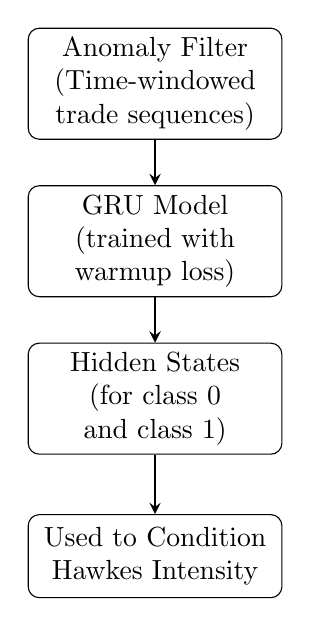
\begin{tikzpicture}[node distance=2cm]

    \tikzstyle{block} = [rectangle, draw, text width=8.5em, align=center, rounded corners, minimum height=3em]
    \tikzstyle{arrow} = [thick,->,>=stealth]

    \node (filtered) [block] {Anomaly Filter\\ (Time-windowed trade sequences)};
 
    \node (gru) [block, below of=filtered] {GRU Model\\ (trained with warmup loss)};

    \node (hidden) [block, below of=gru] {Hidden States\\ (for class 0 and class 1)};

    \node (hawkes) [block, below of=hidden] {Used to Condition\\ Hawkes Intensity};

    \draw [arrow] (filtered) -- (gru);
    \draw [arrow] (gru) -- (hidden);
    \draw [arrow] (hidden) -- (hawkes);

\end{tikzpicture}
\caption{Input-output flow of the GRU-based encoder.}
\label{fig:gru-flow}
\end{figure}

The input-output workflow of this process can be summarized as follows:
\begin{figure}[H]
\centering
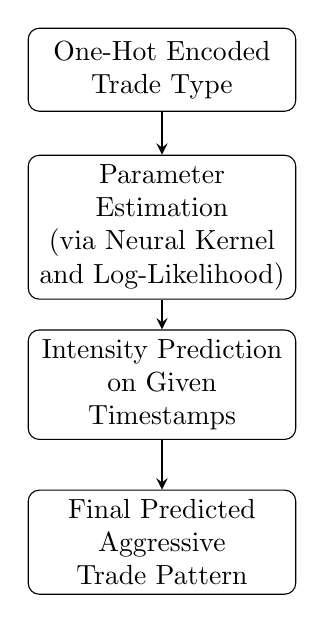
\begin{tikzpicture}[node distance=2cm]
    \tikzstyle{block} = [rectangle, draw, text width=9em, align=center, rounded corners, minimum height=3em]
    \tikzstyle{arrow} = [thick,->,>=stealth]
    \node (onehot) [block] {One-Hot Encoded\\ Trade Type};
    \node (estimate) [block, below of=onehot] {Parameter Estimation\\ (via Neural Kernel and Log-Likelihood)};
    \node (predict) [block, below of=estimate] {Intensity Prediction\\ on Given Timestamps};
    \node (output) [block, below of=predict] {Final Predicted\\ Aggressive Trade Pattern};

    \draw [arrow] (onehot) -- (estimate);
    \draw [arrow] (estimate) -- (predict);
    \draw [arrow] (predict) -- (output);

\end{tikzpicture}
\caption{Input-output flow of the Neural Hawkes Process.}
\label{fig:neural-hawkes-flow}
\end{figure}

\section{Evaluation Metrics} \label{sec:evaluation-metrics}
This section introduces the metrics useful to evaluate how well the predicted aggressive trades resemble the actual ones in the market. Traditional classification metrics, such as precision and recall, assume that each predicted event must match one true event exactly. However, in our case, MN accepts that the prediction of an aggressive trade does not have to be exactly on the timestamp in the data, but can be in an interval around this moment. Thus, I care more about the temporal patterns and distributional behavior of events. For this reason, I include other metrics that can measure similarity in terms of clustering, alignment, and statistical distribution.

As shown in Table~\ref{tb:Evaluation Metrics}, I organize the evaluation into five categories: classification-based metrics, temporal dependency metrics, clustering metrics, autocorrelation, distributional statistical tests.

\begin{table}[h]
\centering
\begin{tabular}{|l|l|l|}
\hline
\textbf{Category} & \textbf{Metric} & \textbf{Purpose} \\
\hline
Classification & Confusion Matrix & Pointwise event match \\
Classification & Precision, Recall, F1-score & Basic prediction quality \\
Temporal Dependency & DTW & Flexible pattern alignment \\
Temporal Dependency & Wasserstein Distance & Distributional shift in timing \\
Temporal Dependency & Fréchet Distance & Curve shape similarity \\
Clustering & Allan Factor & Burstiness and overdispersion \\
Clustering & Event Counts & Count variation in time bins \\
Clustering & Ripley's K Function & Multi-scale clustering test \\
Autocorrelation & Autocorrelation Analysis & Memory and repeated patterns \\
Distributional Test & KS Test & Statistical distribution equality \\
Distributional Test & KL Divergence & Information loss in distributions \\
\hline
\end{tabular}
\caption{Summary of Evaluation Metrics}\label{tb:Evaluation Metrics}
\end{table}

\subsection{Classification-based Metrics}
The confusion matrix shows the number of correctly and incorrectly predicted events. It includes true positives (TP), false positives (FP), true negatives (TN), and false negatives (FN). TP are cases where the model correctly predicts an aggressive event, meaning both the actual and predicted values are one. FP occur when the model predicts an aggressive event, but no actual event happens. TN are when the model correctly predicts non-aggressive trades, with both actual and predicted values being zero. FN happen when an actual aggressive event occurs, but the model fails to detect it, resulting in a missed event. These values help measure how many real events were captured and how many predictions were wrong.

Based on the confusion matrix, I calculate precision, recall, and F1-score. Precision is the proportion of correct predictions out of all predicted events. Recall is the proportion of actual events that were correctly predicted. F1-score is the harmonic mean of precision and recall. However, in our case, these values are not very meaningful because aggressive events are rare and exact matches are unlikely. Still, I include them for completeness.

\subsection{Temporal Dependency Metrics}
Temporal dependency metrics evaluate how well the predicted aggressive trade sequence follows the timing and rhythm of the actual sequence. These metrics are useful when the goal is to match general behavior.

Dynamic Time Warping (DTW) is a technique that allows flexible alignment between two sequences by warping the time axis, making it suitable for comparing patterns that may not align perfectly in time \citep{muller2007dtw}. Wasserstein Distance, also known as Earth Mover's Distance, measures how much 'effort' is needed to move one event timing distribution into another. It is useful for comparing the overall position and spread of events. Fréchet Distance measures the similarity between two event trajectories, considering the order and path taken by events. It focuses more on the global shape than local alignment.

Together, these three metrics provide a more complete evaluation of temporal similarity. DTW captures local flexibility and pattern alignment, Wasserstein Distance reflects distributional shift in timing, and Fréchet Distance focuses on overall shape.

\subsection{Clustering Metrics}
Clustering metrics test whether events happen close together in time, which is a common behavior in financial markets, especially for trader behaviors.

The Allan Factor measures how much the event counts vary in fixed time windows. Values close to one suggest random behavior, while higher values indicate clustering. Event Counts per Fixed Window analyze how many events happen in each time bin (e.g., 1 second, 5 seconds). Ripley's K Function is used to check clustering at multiple time scales. If the K value is higher than expected under randomness, then clustering is present.

Each of these metrics captures clustering from a different perspective. The Allan Factor focuses on overdispersion in event counts over time, Event Counts per Fixed Window provide direct insight into local density, and Ripley's K Function examines clustering across multiple time scales. Using all three allows us to evaluate both short-term and long-term clustering behavior, making the analysis more reliable than using any single metric alone.

\subsection{Autocorrelation Metrics}
Autocorrelation metrics check whether events are dependent on previous events. In market microstructure, it is common to see memory or self-excitation in order flows. Autocorrelation Analysis measures the correlation between an event and its past values. If the correlation is significant at short lags, it suggests that events are not independent.

\subsection{Distributional Statistical Tests}
These tests compare the statistical properties of predicted and actual events. The Kolmogorov-Smirnov (KS) Test compares the cumulative distributions of inter-arrival times. A high p-value means there is no significant difference between the two. Kullback-Leibler Divergence (KL) measures how much information is lost when one distribution is used to represent another. Lower values mean the two distributions are more similar.

While the KS Test provides a formal statistical test for distributional similarity, KL Divergence offers a continuous measure of how much the distributions differ in shape and information. By combining both, I can assess distributional similarity, which leads to a more balanced evaluation than relying on either one alone.




\chapter{Analyses and Results}\label{chapter:experiments}
% \setcounter{page}{0}
% \pagenumbering{arabic}
In this chapter, I present the empirical experiments to test the model. The goal is to test our proposed prediction framework in modeling aggressive trades in the FX spot market. In Section~\ref{sec:prediction}, I present the prediction results from the full framework. It includes: first, an XGBoost model is used to reduce the size of the data and find possible aggressive trades; second, a GRU-based neural network encodes temporal market conditions into hidden states, a Neural Hawkes Process uses these hidden states to estimate the chance of aggressive trades over time. Lastly, Section~\ref{sec:benchmark} compares our model's performance with a benchmark XGBoost classifier without resampling. This shows our approach not only has dynamic prediction ability but also reflects realistic trading behavior in terms of timing, clustering, and statistical distribution.

% Evaluating how well the model captures aggressive trades movements and distribution.
% Market realism (stylized facts: price impact, spread, volume clustering).

\section{Prediction Results} \label{sec:prediction}
The prediction framework consists of three sequential stages. The first stage employs an XGBoost model to identify potential aggressive trade timestamps while reducing the overall dataset size. The second stage is GRU networks. It serves as a bridge between machine learning approaches and stochastic processes. It generates hidden states as neural kernels. The final stage implements a neural Hawkes process that estimates event intensity. In the end this approach produces a detailed and interpretable decision of predictions for aggressive trading events.

% ------------Appendix------------
I present the prediction results of each stage using representative trading days. The training data consists of a whole trading day and the test data consist of random fragment datasets from different days. In this section, the training dataset consists of the whole trading day from January 31, 2025, 10:00:00 to 15:59:59 PM, containing 307,764 rows. This day is chosen because it contains lots of market information and trade data, which is the most comprehensive trading day across the whole dataset. The testing dataset is 30-minute from February 18, 2025, 13:30:04.710 to 13:59:53.060. More testing datasets which are some 30-minute, 1-hour windows from different trading days and each with around 20,000 rows are displayed in Appendix. This specific time window was selected as it represents a commonly used timeframe for FX trading backtesting within the MN platform.

\subsection{XGBoost Stage: With and Without KMeansSMOTE}

KMeansSMOTE, introduced in Chapter~\ref{chapter:methodology}, is an oversampling technique designed to address class imbalance in training data. I compare the XGBoost prediction results with and without KMeansSMOTE to evaluate the influence of oversampling. The impact of applying this oversampling method on both class balance and prediction quality is analyzed.

I first present the classification results of XGBoost trained with KMeansSMOTE. The KMeansSMOTE configuration is as follows:

\begin{verbatim}
pipeline = Pipeline([
("imputer", SimpleImputer(strategy="median")),
("smote", KMeansSMOTE(random_state=42,
cluster_balance_threshold=0.02,
kmeans_estimator=KMeans(n_clusters=200, random_state=42),
sampling_strategy=0.5))
])
\end{verbatim}

The median strategy fills missing values with the median of each feature. A cluster balance threshold of 0.02 ensures oversampling is done in 'safe' areas where there are at least some genuine minority examples. As a result, the training set has the ratio of 3:7 about class 1 and class 0. It significantly increases the class balance from 1:499 in Figure~\ref{fig: aflag_class_distribution}.

% !!maybe need refinement
This step is aimed to get a model to initially find out as many positives as possible by keeping recall as 0.6 without losing precision. So, the input for testing only depends on market features ($S$, $M$, $V_A^{1}$, $V_A^{1}$, $\bar{\delta}_S$, $\bar{\delta}_M$, $\sigma_S$, $\sigma_M$, $r_V$), and the output contains the shortened training dataset for the next step with aggressive trade candidates. The filtered output also gets rebalanced towards class 1 because I filter out those are not predicted as 1. the bias toward class 0 and helps the model learn better from the underrepresented class 1.

As shown in Figure~\ref{fig:xgb-pred-vs-true-km}, KM-XGBoost catches many true positives. The class balancing done by KMeansSMOTE reduces the bias toward class 0 and helps the model learn better from the underrepresented class 1.

Table~\ref{tab:xgb-confusion-km} shows the confusion matrix. 4,011 are predicted as class 0 (non-aggressive trade), and 3,739 are predicted as class 1. The model correctly finds 13 true positives and 4,001 true negatives. I exclude those which are not predicted as class 1, so the testing dataset size drops from 7,750 to 3,739 rows, which is 51.75\% of the original. This helps improve speed and keeps most of the important trade points, and make preparation for prediction in the next neural Hawkes process.

Moreover, Table~\ref{tab:xgb-classification-report-km} shows the detailed classification report. I mainly care about the prediction performance for class 1, since this is the main goal of the whole research. The precision of class 0 is not meaningful here because the original data is extremely imbalanced. Although the precision for class 1 is still very low at 0.0035, the recall reaches 0.5652. This means the model finds sufficient true trades under the model with oversampling. This makes preparation for next neural Hawkes process.

In Table~\ref{tab:xgb-noKM}, without KMeansSMOTE, even if I reach the same recall, the precision is even worse (only 0.0019). This value means almost all predicted class 1 are wrong. The F1-score is just 0.0038, which is only half of the score from XGBoost with KMeansSMOTE. Also, the filter effect is weaker. More lines (5,065) are left in the result, which makes the next detection step slower and more difficult. So using KMeansSMOTE helps not only improve model performance but also makes the pipeline more efficient.

\begin{figure}[H]
    \centering
    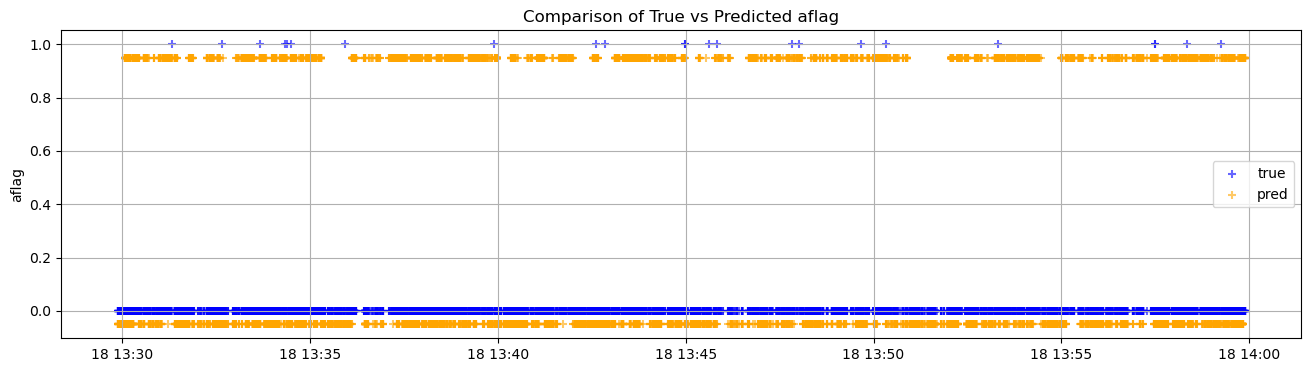
\includegraphics[width=\textwidth]{figures/aflag_XGBoost_181330.png}
    \caption{Comparison of true vs. predicted $\bar{\alpha}$ from XGBoost with KMeansSMOTE} 
    \caption*{\textit{Note:} The blue '+' markers show the true class labels, and the orange '+' markers show the predicted ones. To make the plot easier to read, the predicted values are moved down by 0.05 on the y-axis.  The prediction catches most of the true values.
    }
    \label{fig:xgb-pred-vs-true-km}
\end{figure}

\begin{table}[H]
    \centering
    \caption{Confusion matrix of XGBoost with KMeansSMOTE}
    \caption*{\textit{Note:} The confusion matrix from the XGBoost model trained with KMeansSMOTE to handle class imbalance. The model correctly predicts 4,001 true negatives (class 0) and 13 true positives (class 1). It misclassifies 3,726 instances as aggressive trades and misses 10 true aggressive events. In total, 3,739 rows are predicted as class 1, which is 51.75\% of the original test set size of 7,750. This filtered output keeps most of the important aggressive trade candidates and reduces data size for the next step in the neural Hawkes process.}
    \label{tab:xgb-confusion-km}
    \begin{tabular}{lcc}
        \toprule
        & Predicted 0 & Predicted 1 \\
        \midrule
        True 0 & 4,001 & 3,726 \\
        True 1 & 10 & 13 \\
        \bottomrule
    \end{tabular}
\end{table}

\begin{table}[H]
    \centering
    \caption{Classification report of XGBoost with KMeansSMOTE}
    \caption*{\textit{Note:} The classification performance of the XGBoost model trained with KMeansSMOTE. The main focus is on class 1, which represents aggressive trades. Although the precision for class 1 is very low (0.0035), the recall reaches 0.5652, meaning the model captures more than half of the true aggressive events. This is important because the data is extremely imbalanced, and the goal is to find as many true trades as possible for the next stage in the neural Hawkes process. The precision of class 0 is not meaningful due to the imbalance. Overall accuracy is 51.79\%, but recall for class 1 is the key metric here.}

    \label{tab:xgb-classification-report-km}
    \begin{tabular}{lcccc}
        \toprule
        Class & Precision & Recall & F1-score & Support \\
        \midrule
        0 & 0.9962 & 0.5178 & 0.6817 & 7727 \\
        1 & 0.0035 & 0.5652 & 0.0069 & 23 \\
        \midrule
        Accuracy & \multicolumn{4}{c}{0.5179} \\
        \bottomrule
    \end{tabular}
\end{table}

\begin{table}[H]
    \centering
    \caption{Confusion matrix of XGBoost without KMeansSMOTE}
    \caption*{\textit{Note:} The classification performance of the XGBoost model without using KMeansSMOTE. When the recall for class 1 remains similar (0.5881), the precision drops to 0.0019. The F1-score is 0.0038, which is only half of the score obtained when using KMeansSMOTE. In addition, the model leaves 5,065 rows in the output, which reduces filtering effectiveness and increases the computational burden for the next detection step.}
    \label{tab:xgb-noKM}
    \begin{tabular}{lccc}
        \toprule
        Class & Precision & Recall & F1-score\\
        \midrule
        1 & 0.0019 & 0.5881 & 0.0038 \\        
        \bottomrule
    \end{tabular}
\end{table}

In conclusion, these results show that KMeansSMOTE gives significant improvement when dealing with extreme class imbalance, especially in terms of F1-score. I can also infer from the classification evaluation that single XGBoost is not enough for the prediction task even with resampling methods. The large set of candidate points predicted at this stage will be passed to the next neural Hawkes model, which helps to further clean and refine the aggressive trade signals. 

\newpage

%------------- Neural Hawkes process -------------
\subsection{Neural Hawkes Process Results}
I use the GRU model to generate hidden states as a neural kernel, which are then used in the Hawkes process. In this stage, I refer to the training process as estimation and testing process as prediction, since it involves fitting a Hawkes process. The estimation (training) is performed on the dataset from January 31, 2025, between 10:00:00 and 15:59:59. This period is the same as the XGBoost training set, but the data is filtered using the XGBoost filter to reduce class imbalance.

In the estimation stage, the GRU is trained as mentioned in Chapter~\ref{chapter:methodology} and hidden states $h_t$ are extracted. For estimation in next Hawkes process, Figure~\ref{fig:train-hidden-state} depicts the hidden states generated from GRU.

In the estimation stage, the GRU is trained as described in Chapter~\ref{chapter:methodology}, and the hidden states $h_t$ are extracted for each time step. These hidden states serve as a compressed representation of the input dynamics and are used as input features for the Hawkes process parameter estimation. The hidden states are transformed using the function $\log(1 + e^{h_k(t)})$ as in Formula~\ref{eq:intensity}. Figure~\ref{fig:train-hidden-state} depicts the hidden states generated from the GRU, separated by class. The top panel shows the hidden state for class 0 (non-aggressive events), while the bottom panel displays the hidden state for class 1 (aggressive events). Compared to class 0, the hidden state for class 1 shows smoother trends and more distinct spikes, which may help the Hawkes process distinguish aggressive event patterns more effectively in the next stage.

\begin{figure}[H]
    \centering
    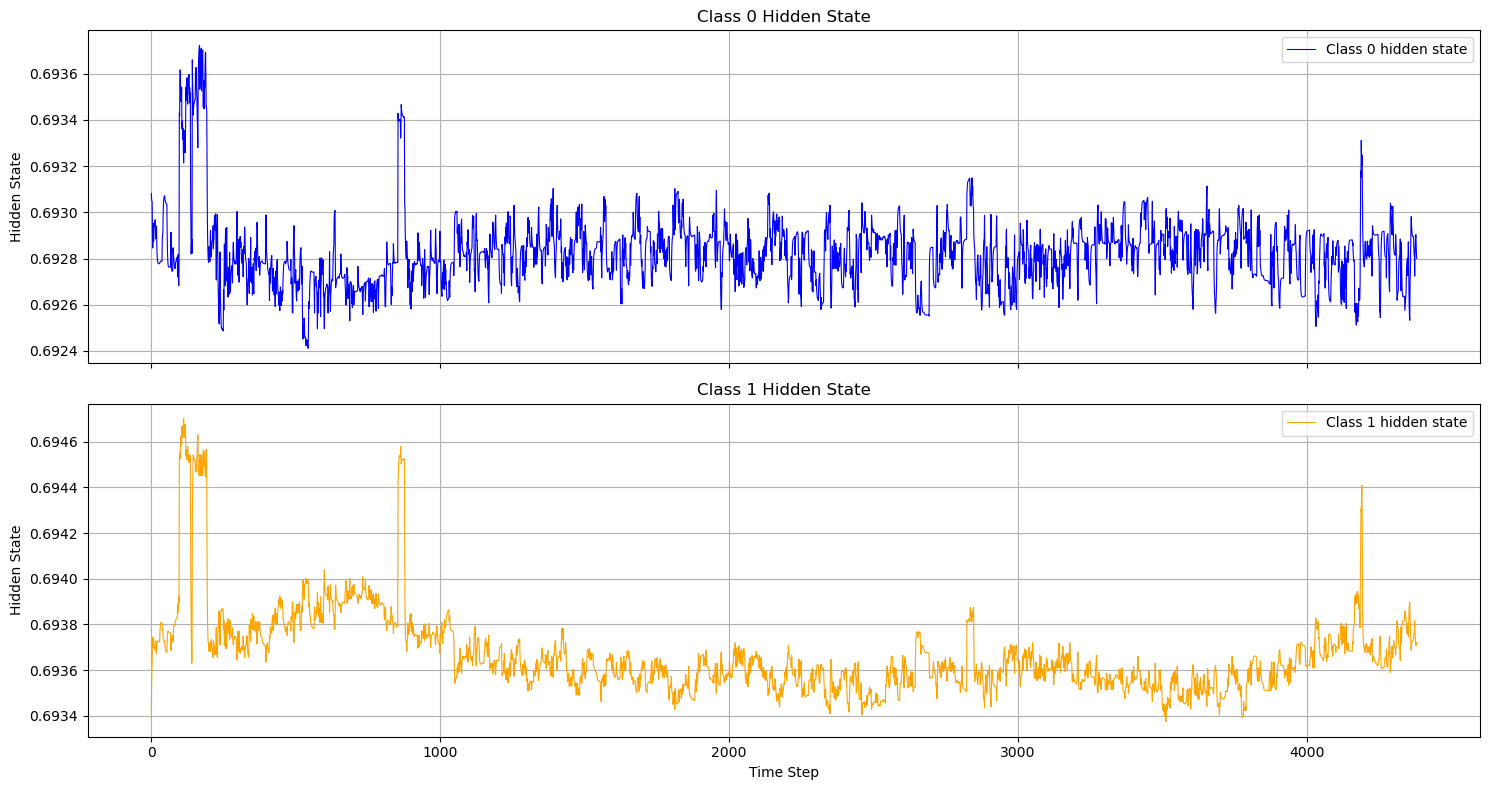
\includegraphics[width=0.95\linewidth]{figures/train-hidden-state.png}
    \caption{Hidden state for estimation dataset of each event type}
    \caption*{\textit{Note:} The top panel shows the hidden state for class 0 (non-aggressive events), while the bottom panel displays the hidden state for class 1 (aggressive events).}
    \label{fig:train-hidden-state}
\end{figure}


These hidden states are passed to the Hawkes intensity formula in Equation~\ref{eq:intensity}. I estimate the parameters by minimizing the negative log-likelihood using the L-BFGS-B method. The optimization process completed in 363.98 seconds, the final negative log-likelihood reached $-8261.28$, and success flag returned \texttt{True} which means it successfully get convergence. The estimated results are as follows:
\begin{table}[H]
    \centering
    \caption{Estimated Parameters of the Neural Hawkes Process}
    \caption*{\textit{Note:} The estimated parameters of the neural Hawkes process. The baseline intensity $\mu$ shows that non-aggressive trades (Type 0) are more likely to occur by default than aggressive trades (Type 1). The excitation matrix $\alpha$ captures how one trade type increases the likelihood of another trade type. Aggressive trades have a strong self-excitation ($\alpha_{1,1} = 2.57$) and also increase the chance of non-aggressive trades ($\alpha_{0,1} = 15.85$). Non-aggressive trades have little effect on aggressive ones ($\alpha_{1,0} = 0.52$). The decay matrix $\beta$ tells us how quickly these effects fade. Aggressive trades have a short but strong influence on others, while non-aggressive trades influence aggressive trades only briefly.}
    \label{tb:hawkes-params}
    \begin{tabular}{lcc}
    \toprule
    \textbf{Parameter} & \textbf{Type 0 (Non-Aggressive)} & \textbf{Type 1 (Aggressive)} \\
    \midrule
    \multicolumn{3}{l}{\textbf{Baseline Intensity} (\( \mu \))} \\
    \quad Value & 0.0677 & 0.0029 \\
    \midrule
    \multicolumn{3}{l}{\textbf{Excitation Matrix} (\( \alpha \))} \\
    \quad From Type 0 & 10.12 & 0.52 \\
    \quad From Type 1 & 15.85 & 2.57 \\
    \midrule
    \multicolumn{3}{l}{\textbf{Decay Matrix} (\( \beta \))} \\
    \quad From Type 0 & 10.55 & 62.32 \\
    \quad From Type 1 & 18.48 & 14.76 \\
    \bottomrule
    \end{tabular}
\end{table}

Results of the baseline intensity $\mu$ mean the natural chance of a non-aggressive trade is higher than an aggressive trade without any past event influence. In our case, non-aggressive trades are more likely to occur by default with $\mu_0 = 0.0677$, while aggressive trades are rare ($\mu_1 = 0.0029$) and usually triggered by certain market activity otherwise less easy to happen naturally.

For excitation matrix $\alpha$, the first column shows how past events of both types excite type 0 (non-aggressive), and the second column shows how they excite type 1 (aggressive). An aggressive trade (type 1) causes a strong self-excitation (2.57), but non-aggressive trade has much smaller influence on aggressive one (0.52). Surprisingly, for non-aggressive trade, cross-excitation from aggressive to non-aggressive (15.85) is higher than its self-excitation. This reflects aggressive trade events have significant market influence both to themselves and to non-aggressive trades.

Each value in the decay matrix $\beta$ represents how quickly the effect of a past event of type fades when it influences the intensity of current type. A non-aggressive trade (type 0) decays with a moderate speed when it influences another non-aggressive trade (\( \beta = 10.55 \)). When an aggressive trade (type 1) influences non-aggressive activity (\( \beta = 18.48 \)), the effect decays faster. Combined with the $\alpha = 15.85$, it suggests that aggressive trade has a short but noticeable impact for non-aggressive trade in the market. On the other hand, a non-aggressive trade has almost no lasting effect on aggressive trades, as shown by the very fast decay rate (\( \beta = 62.32 \)). Lastly, the self-decay for aggressive trades (\( \beta = 14.76 \)) is moderate, meaning aggressive trades cluster, but the effect also wears off gradually.


% ----------------estimated intensity plot------------------
% !!need careful explain of this plot
Figure~\ref{fig:neuralhp-intensity} shows the result of the intensity estimation based on the fitted model and the hidden states from GRU. It is generated by computing the intensity at evenly spaced timestamps over the trading period, and only 1,750 steps are shown here. The model uses the hidden state $h_t$ from GRU at each time point, along with the event history up to that point, to calculate the intensity values. 

The top plot is the sum of intensities $\sum_{m} \lambda_k(t)$ across both event types at every time step. The small purple markers indicate when actual events occurred. The middle plot shows the intensity for type 0 (non-aggressive). It has strong fluctuations and many large peaks. It aligns well with the red event markers. As can be seen in the bottom plot, it is type 1 (aggressive) intensity, which is generally much lower than non-aggressive trade events. Still, many aggressive trade events align with sharp local peaks, meaning the model successfully captures those trades. In conclusion, the estimation results show that the model correctly adjusts intensity to reflect aggressive trade likelihood.

\begin{figure}[H]
    \centering
    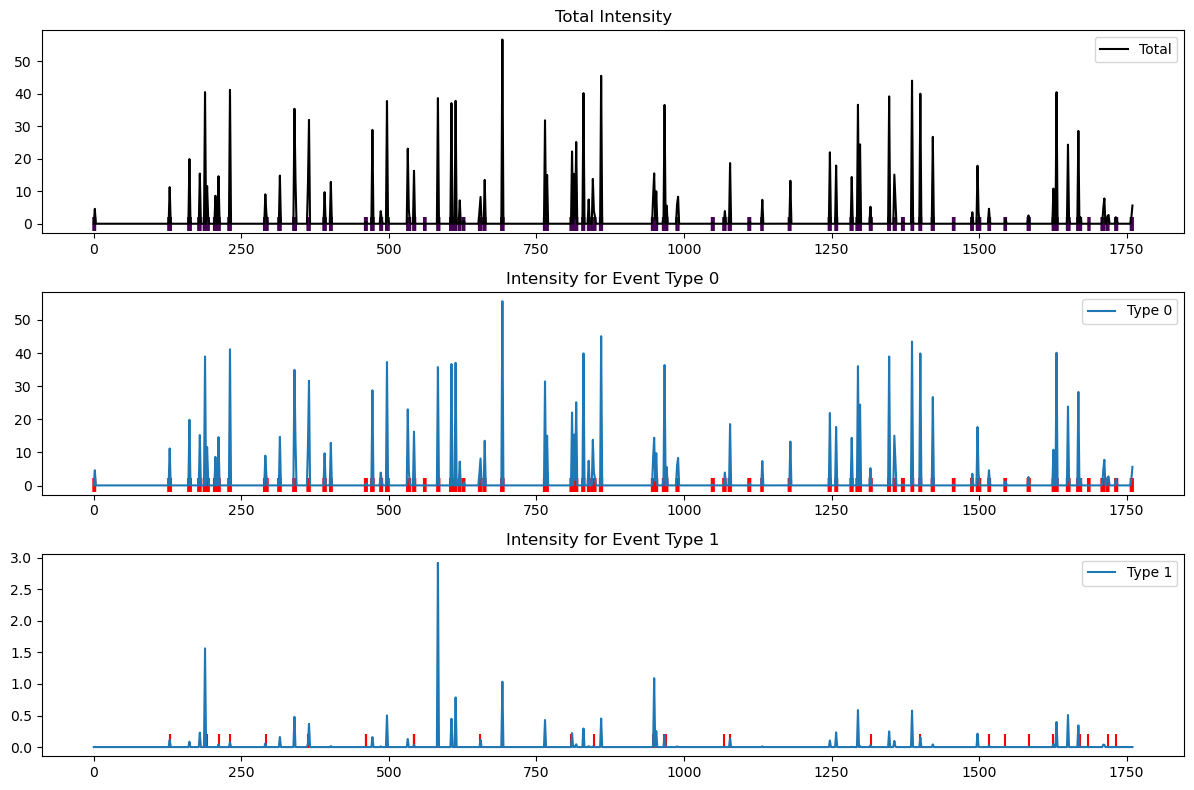
\includegraphics[width=0.95\linewidth]{figures/hp_estimation.png}
    \caption{Estimated intensity functions for each event type}
    \caption*{\textit{Note:} This figure shows the estimated intensity functions from the neural Hawkes process. Only 1,750 time steps are shown for clarity. The top plot shows the total intensity across both types. Small purple markers show when events occurred. The middle plot shows the intensity for non-aggressive trades (type 0), which has many peaks and follows the event markers well. The bottom plot shows the intensity for aggressive trades (type 1), which is much lower, but still shows peaks at the correct times.}

    \label{fig:neuralhp-intensity}
\end{figure}
\newpage
%------------ prediction -------------
After getting the estimated parameters from the training phase, I test the Neural Hawkes Process on out-of-sample data. The input for prediction comes from the out-of-sample output of the XGBoost classifier. This XGBoost, as discussed before, is designed to contain more aggressive trades by predicting as many positives as possible, helping us balance the class better during prediction. It includes market features such as spread ($S$), mid-price ($M$), volume at best ask and bid ($V_A^1$, $V_B^1$), short-term average changes ($\bar{\delta}_S$, $\bar{\delta}_M$), volatilities ($\sigma_S$, $\sigma_M$), and volume ratio ($r_V$). These can all be fetched directly from Snowflake or calculated by these raw data. These features are used to extract hidden states from the GRU, and the corresponding timestamps ($T$) are passed into the Hawkes process to compute event intensities using the previously estimated parameters.

I first conduct prediction on a sample from 2025-02-18 13:30:04.710 to 2025-02-18 13:59:53.060. The model finally predicts 38 points as aggressive trades. In reality, 23 of them are actual aggressive trades during this time window. It is acceptable because it is more tolerant for false positives than false negatives. The prediction result is in Figure~\ref{fig:nhp-aflag}.

\begin{figure}[H]
    \centering
    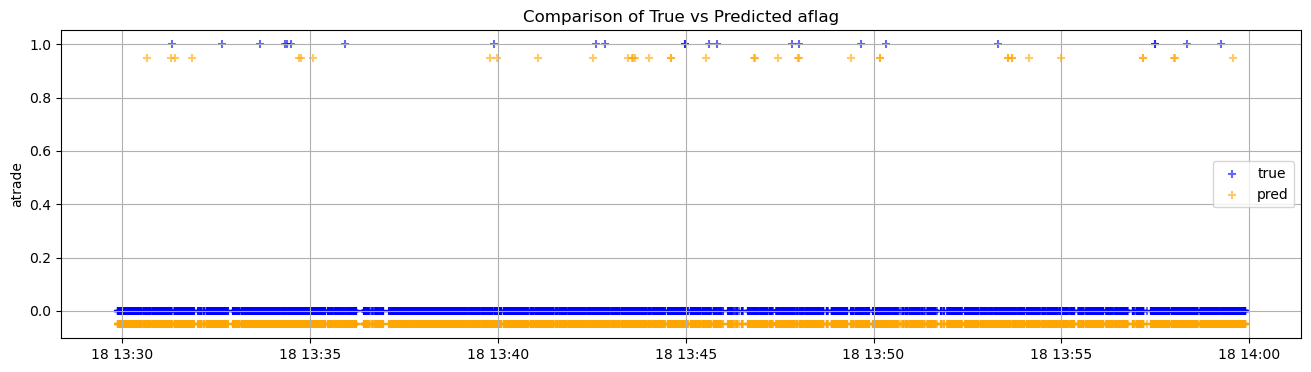
\includegraphics[width=0.9\linewidth]{figures/aflag_NHP_181330.png}
    \caption{Comparison of true vs. predicted $\bar{\alpha}$ from neural Hawkes process} 
    \caption*{\textit{Note:} The blue '+' markers show the true class labels, and the orange '+' markers show the predicted ones. To make the plot easier to read, the predicted values are moved down by 0.05 on the y-axis.
    }
    \label{fig:nhp-aflag}
\end{figure}



\subsection{Performance Evaluation}
When it comes to performance evaluation, relying on exact matching metrics like confusion matrix, precision, or recall is not sufficient. In our case, the model predicts 38 aggressive trades while only 23 are truly observed. This difference is expected because the neural Hawkes process simulates events based on the fitted intensity. Its purpose is to capture realistic market patterns, rather than replicate the exact event sequence. In the MN backtesting context, it is more important to match the overall temporal behavior and shape of trading activity than to align precisely with every timestamp. Below, I explain the results of more appropriate evaluation metrics, as summarized in Table~\ref{tb:Evaluation Metrics}.

%----------Temporal Alignment---------
The \textbf{Dynamic Time Warping (DTW)} distance is 23.0, with a normalized DTW value of 0.00297 in Table~\ref{tab:dtw}. This is very low, which shows that the predicted trade activity follows a very similar time pattern as the actual aggressive trades. The alignment path length is 15,464, and the diagonal ratio is 1.995. A ratio close to 2 means the predicted and actual sequences align almost one-to-one. These results confirm that the model learns the shape and rhythm of the trading activity well.
\begin{table}[H]
    \centering
    \caption{Dynamic Time Warping (DTW) Results} \label{tab:dtw}
    \caption*{\textit{Note:} The results from DTW. The DTW distance is 23.0, and the normalized distance is 0.00297. This small value means the predicted trades follow a very similar time pattern as the true ones. The diagonal ratio is 1.995. A ratio near 2 means the predicted and actual events align almost one-to-one.}
    \begin{tabular}{lr}
    \toprule
    Metric & Value \\
    \midrule
    DTW Distance & 23.0 \\
    Normalized DTW Distance & 0.00297 \\
    Alignment Path Length & 15,464 \\
    Diagonal Ratio & 1.995 \\
    \bottomrule
    \end{tabular}
\end{table}

The \textbf{Wasserstein distance} is 0.0019 in Table~\ref{tb:wasserstein-results}, and the normalized value is also 0.0019 out of a possible maximum distance of 1.0. This is extremely low. It means that the distribution of predicted event times is almost the same as the real distribution. This is a very strong result, showing that even if the model doesn't predict every individual event correctly, the timing and density of trades over time is very accurate.
\begin{table}[H]
    \centering
    \caption{Wasserstein Distance Results}
    \caption*{\textit{Note:} The Wasserstein distance between the predicted and actual distributions of aggressive trade times. The distance is 0.0019, and the normalized value is also 0.0019 out of a maximum of 1.0. This is extremely low, which means the predicted timing and density of trade events are very close to the real ones. Even if the model does not capture every single event, the overall distribution pattern over time is very accurate.}
    \label{tb:wasserstein-results}
    \begin{tabular}{lr}
    \toprule
    Metric & Value \\
    \midrule
    Wasserstein Distance & 0.0019 \\
    Normalized Distance & 0.0019 \\
    Maximum Possible Distance & 1.0000 \\
    \bottomrule
    \end{tabular}
\end{table}

% For the \textbf{Fréchet distance} in Table~\ref{tb:frechet-results}, the value is 120.98 and the normalized value is 0.4263. This is a higher value compared to DTW or Wasserstein, which suggests that while the general pattern is followed, the paths are not perfectly smooth or identical. Still, it is within an acceptable range for modeling real-world stochastic processes. The model predicts 37 event intervals, while there are 22 in reality, indicating a slight over-generation of events. However, the Kolmogorov-Smirnov (KS) test p-value is 0.1239, which means the model's event interval distribution is not statistically different from the true one at common significance levels.
% \begin{table}[H]
%     \centering
%     \caption{Fréchet Distance and Distribution Comparison}
%     \label{tb:frechet-results}
%     \begin{tabular}{lr}
%     \toprule
%     Metric & Value \\
%     \midrule
%     Fréchet Distance & 120.98 \\
%     Fréchet Distance (Normalized) & 0.4263 \\
%     Wasserstein Distance (Reference) & 30.99 \\
%     KS Test p-value & 0.124 \\
%     Actual Intervals & 22 \\
%     Predicted Intervals & 37 \\
%     \bottomrule
%     \end{tabular}
% \end{table}

In summary, these metrics show that our model captures the dynamics and timing patterns of aggressive trades well. While not perfect in predicting exact events, the low DTW and Wasserstein distances confirm strong temporal alignment and distributional similarity. This supports the usefulness of our model for predicting trader behavior in backtesting environments.



%-------------------clustering---------------------
To further evaluate the realism of the predicted aggressive trades, I assess the clustering behavior using two statistical tools: the Allan Factor and Ripley's K/L functions. These methods help us understand whether the predicted results have realistic temporal clusters like the reality in the market, or whether they behave more like random noise.

The \textbf{Allan factor} measures event clustering over different time windows. A value of AF greater than 1 indicates clustering, while AF close to 1 suggests a random process. As can be seen in Table~\ref{tb:allan-factor}, for the true aggressive trades ($\bar{\alpha}_\text{true}$), the average Allan Factor is 1.0698. The Allan Factors across different window sizes are as follows: 1.044 for window size 2, 1.044 for window 5, 0.958 for window 10, 1.090 for window 20, and 1.050 for window 50. This suggests consistent clustering in the actual events. For the predicted aggressive trades ($\bar{\alpha}_\text{pred}$), the average Allan Factor is higher, at 1.2687. The Allan Factors at various window sizes are: 0.869 at window size 2, 1.290 at window 5, 1.159 at window 10, 1.346 at window 20, and 1.722 at window 50. These values show stronger clustering in the prediction, especially at longer windows. This is reasonable, as the neural Hawkes process is designed to model self-exciting behavior especially.

\begin{table}[H]
    \centering
    \caption{Allan Factor Results for Aggressive Trade Clustering}
    \caption*{\textit{Note:} The Allan Factor (AF) values for both true and predicted aggressive trades across different window sizes. An AF greater than 1 indicates clustering. For the true trades ($\bar{\alpha}_\text{true}$), the average AF is 1.0698. The predicted trades ($\bar{\alpha}_\text{pred}$) have a slightly higher average AF of 1.2687. This difference is expected, since the neural Hawkes process models self-exciting behavior.}
    \label{tb:allan-factor}
    \begin{tabular}{lcc}
    \toprule
    \textbf{Window Size} & $\bar{\alpha}_\text{true}$ & $\bar{\alpha}_\text{pred}$\\
    \midrule
    2   & 1.044 & 0.869 \\
    5   & 1.044 & 1.290 \\
    10  & 0.958 & 1.159 \\
    20  & 1.090 & 1.346 \\
    50  & 1.050 & 1.722 \\
    \midrule
    \textbf{Average AF} & 1.0698 & 1.2687 \\
    \textbf{Number of Events} & 23 & 38 \\
    \textbf{Event Rate} & 0.00297 & 0.00490 \\
    \bottomrule
    \end{tabular}
\end{table}

I also use \textbf{Ripley's K and L functions} to further test clustering. These functions evaluate how events are spread in time. If the \( L(r) \) value is greater than 0, the process is considered clustered; if it is near 0, the process is closer to random. In Table~\ref{tb:ripley-l}, for $\bar{\alpha}_\text{true}$, the number of events is 23, the event intensity is 0.0128 events per second, and the average \( L(r) \) value is 22.76. The values at 1s, 2s, and 5s distances are 12.61, 11.61, and 15.42 respectively. For $\bar{\alpha}_\text{pred}$, the number of events is 38, the intensity is 0.0211 events per second, and the average \( L(r) \) is 31.04. The values at the same distances are 13.96 at 1s, 15.45 at 2s, and 22.42 at 5s. These consistently higher \( L(r) \) values again show stronger clustering in the predicted trades. In the Figure~\ref{fig:ripley-kl}, the blue curve corresponds to the actual aggressive trades, while the orange curve shows the predicted trades generated by the neural Hawkes model. I observe that both curves are consistently above the baseline, indicating clustering behavior in both series. The predicted trades closely match the clustering pattern of the actual trades, particularly at shorter distances. This suggests that the model captures the clustering of aggressive trading activity well.

In conclusion, both Allan Factor and Ripley's L function results suggest that the predicted aggressive trades exhibit realistic clustering behavior. While the predicted clustering is slightly stronger than in the true data, this is a natural result of the self-exciting nature of the Hawkes process.

\begin{table}[H]
    \centering
    \caption{Ripley's L Function Summary}
    \caption*{\textit{Note:} The clustering results based on Ripley's L function for both actual and predicted aggressive trades. If \( L(r) \) is greater than 0, it indicates clustering. For true trades ($\bar{\alpha}_\text{true}$), the average \( L(r) \) is 22.76, while for predicted trades ($\bar{\alpha}_\text{pred}$), the average is 31.04. The values at different time distances (1s, 2s, 5s) are also higher for the predictions, showing that the model produces stronger clustering.}
    \label{tb:ripley-l}
    \begin{tabular}{lcc}
    \toprule
    \textbf{Metric} & $\bar{\alpha}_\text{true}$ & $\bar{\alpha}_\text{pred}$ \\
    \midrule
    Number of Events & 23 & 38 \\
    Event Intensity (events/sec) & 0.0128 & 0.0211 \\
    Average \( L(r) \) & 22.76 & 31.04 \\
    \( L(1s) \) & 12.61 & 13.96 \\
    \( L(2s) \) & 11.61 & 15.45 \\
    \( L(5s) \) & 15.42 & 22.42 \\
    \bottomrule
    \end{tabular}
\end{table}

\begin{figure}[H]
    \centering
    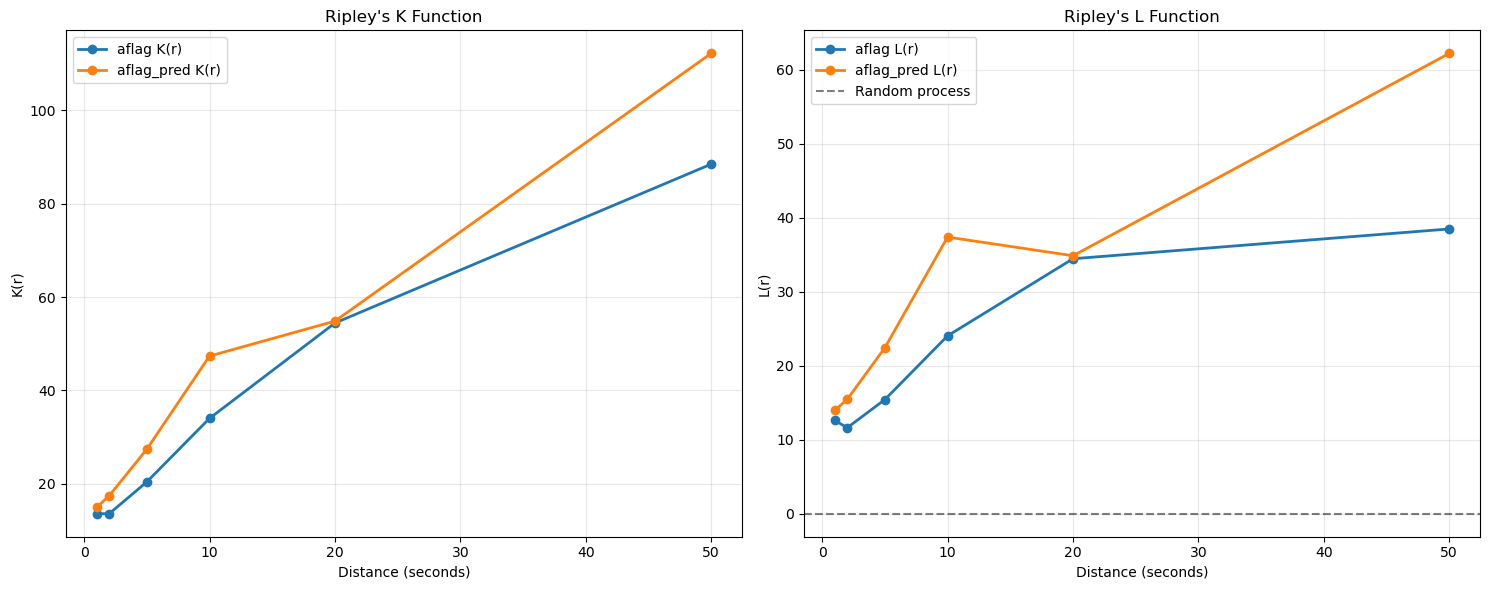
\includegraphics[width=\linewidth]{figures/RIPLEY_181330.png}
    \caption{Ripley's K and L functions comparing real and predicted aggressive trades}
    \caption*{\textit{Note:} Values above the dashed line in the \( L(r) \) plot indicate clustering behavior. Both actual and predicted series exhibit clustering across all distances. The predicted trades show stronger clustering, especially at larger distances, which is consistent with the self-exciting nature of the Hawkes process.}
    \label{fig:ripley-kl}
\end{figure}



%----------------------ACF--------------------
Next, I analyse the \textbf{autocorrelation} structure of both the actual and predicted aggressive trade series to assess whether the neural Hawkes process model shows the temporal dependence between trades. The Autocorrelation Function (ACF) and Partial Autocorrelation Function (PACF) plots are shown in Figure~\ref{fig:acf-pacf}. For the actual aggressive trade series ($\bar{\alpha}_\text{true}$), the lag-1 autocorrelation is 0.0842, showing weak but positive short-term dependence. The values quickly drop near zero at higher lags. For example lag-5 and lag-10 both are -0.0030. In total, 6 lags are statistically significant, and the Ljung-Box test p-value is essentially zero. This indicates that even though the autocorrelations are small, the actual process does have significant temporal structure. Next I test if the temporal structure also exists in our prediction. For the predicted series ($\bar{\alpha}_\text{pred}$), the lag-1 autocorrelation is 0.0744, which is very close to the actual series. Lag-5 and lag-10 values are -0.0049, also similar to the actual values. There are 4 significant lags, and the Ljung-Box test again returns a p-value closing to 0. This indicates the presence of temporal dependence.

These results suggest that the neural Hawkes process produces a time series with similar short-term dependency structure as the actual trader behaviors in the real market. It is fair to say the neural Hawkes process is capable of capturing temporal structure in aggressive trade patterns.

% \textbf{Cross-correlation Analysis:} The cross-correlation between the true and predicted series is also computed. The maximum cross-correlation value is 0.0980, occurring at lag 49. The zero-lag correlation is 0.0301. Although the absolute correlation is small, this shows that the predicted sequence partially aligns with the actual series, especially with a slight time shift.

\begin{figure}[H]
    \centering
    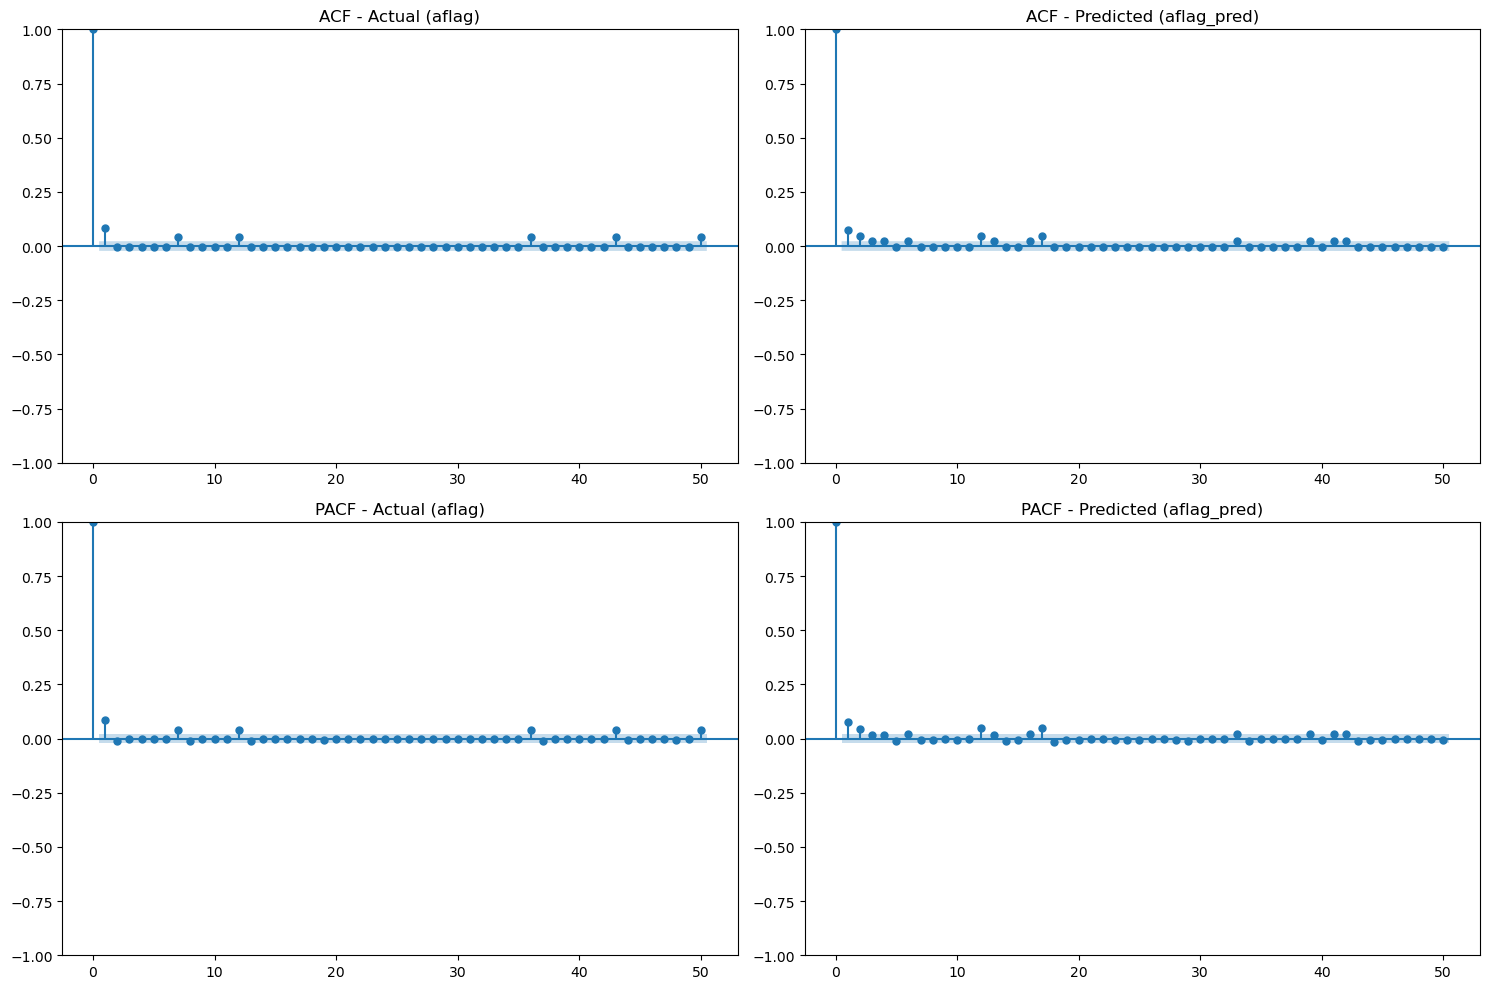
\includegraphics[width=0.95\linewidth]{figures/ACF_181330.png}
    \caption{Autocorrelation (ACF) and Partial Autocorrelation (PACF) plots of actual and predicted aggressive trade series.}
    \caption*{\textit{Note:} The ACF and PACF plots for both the actual and predicted aggressive trade series. The actual series ($\bar{\alpha}_\text{true}$) has a lag-1 autocorrelation of 0.0842, while the predicted series ($\bar{\alpha}_\text{pred}$) has 0.0744. Higher lag values like lag-5 and lag-10 are close to zero or slightly negative in both cases. In total, 6 lags are significant for the actual series and 4 for the predicted one. The Ljung-Box test p-values are close to 0 in both cases, showing that there is meaningful temporal dependence.}
    \label{fig:acf-pacf}
\end{figure}


%----------------Distributional Test-------------

Furthermore, to evaluate how well the predicted aggressive trade events match the statistical distribution of actual trades, I perform distributional tests by the \textbf{Kolmogorov-Smirnov (KS) test}. 
% and the \textbf{Kullback-Leibler (KL) divergence}.

The KS test is used to compare the cumulative distributions of two sample sets. It returns a test statistic and a p-value. If the p-value is below 0.05, the distributions are considered significantly different. In our case as shown in Table~\ref{tb:ks-test}, the KS statistic is 0.0019 and the p-value is 1.0000, indicating that there is no statistically significant difference between the predicted and actual event distributions. The actual proportion of aggressive trades is 0.0030, and the predicted proportion is 0.0049. The difference between them is only 0.0019. This result shows that the neural Hawkes model accurately matches the distribution of aggressive trade occurrence over time.

\begin{table}[H]
    \centering
    \caption{Kolmogorov--Smirnov Test Results}
    \caption*{\textit{Note:} The result of the Kolmogorov-Smirnov (KS) test, which compares the distribution of predicted and actual aggressive trade events. The KS statistic is 0.0019 and the p-value is 1.0000, which means there is no significant difference between the two distributions. The actual proportion of aggressive trades is 0.0030, and the predicted proportion is 0.0049. Their difference is very small, only 0.0019, meaning the neural Hawkes model successfully captures the statistical distribution of aggressive trade events.}
    \label{tb:ks-test}
    \begin{tabular}{lr}
    \toprule
    \textbf{Metric} & \textbf{Value} \\
    \midrule
    KS Statistic & 0.0019 \\
    p-value & 1.0000 \\
    Significant ($p < 0.05$) & False \\
    Actual Proportion & 0.0030 \\
    Predicted Proportion & 0.0049 \\
    Proportion Difference & 0.0019 \\
    \bottomrule
    \end{tabular}
\end{table}

% KL divergence is a measure of how one probability distribution differs from another. I compute the KL divergence in both directions between the windowed count distributions of the predicted and actual events. 

% The value of KL (actual $\parallel$ predicted) is 7.7609 bits, while KL (predicted $\parallel$ actual) is 2.6656 bits. The symmetric KL divergence is 5.2132 bits. These values are relatively moderate, indicating that the predicted distribution is somewhat more peaked or uneven than the actual one. Still, the predicted distribution resembles the actual distribution well enough for backtesting purposes. Lower KL divergence values generally mean higher similarity, and in our case the distributional shape is captured to a reasonable degree.

% \begin{figure}[H]
%     \centering
%     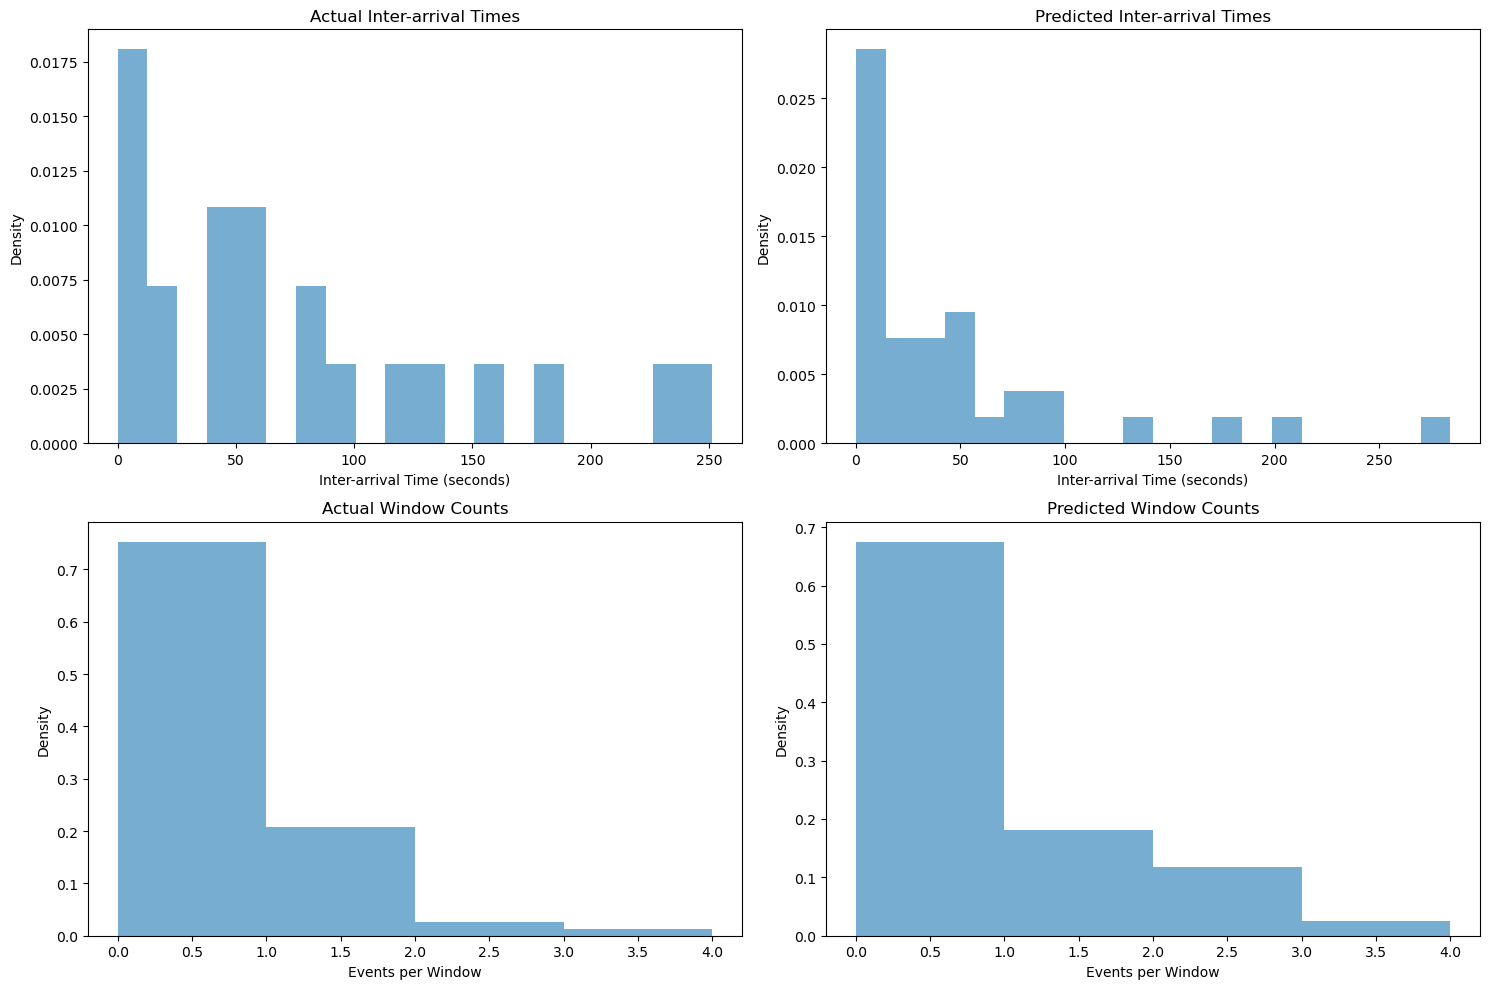
\includegraphics[width=0.95\linewidth]{figures/KL_181330.png}
%     \caption{KL divergence plot for event count distributions (predicted vs actual).}
%     \label{fig:kl-divergence}
% \end{figure}

% \begin{table}[H]
%     \centering
%     \caption{Kullback--Leibler Divergence Between Actual and Predicted Distributions}
%     \label{tb:kl-divergence}
%     \begin{tabular}{lr}
%     \toprule
%     \textbf{Metric} & \textbf{Value (bits)} \\
%     \midrule
%     KL(actual $\parallel$ predicted) & 7.7609 \\
%     KL(predicted $\parallel$ actual) & 2.6656 \\
%     Symmetric KL Divergence & 5.2132 \\
%     \bottomrule
%     \end{tabular}
% \end{table}


%---------Conclusion-----------
Overall, all these metrics, including DTW, Wasserstein distance, Allan factor, Ripley's K and L functions, autocorrelation and KS test confirm that the neural Hawkes process not only models the timing and clustering of events, but also captures the underlying distributional structure of aggressive trade frequency. The Neural Hawkes Process with XGBoost filter and GRU kernel captures realistic and reliable patterns in aggressive trade. It shows interpretable dynamics like short-term excitation, quick decay, and clustering, especially for aggressive trades. This supports our idea that using our framework not only captures overall market features and temporal dependency, but also gives more robustness and control than black-box classifiers.


\newpage

\section{Benchmark Comparison} \label{sec:benchmark}
% \section{Benchmark Model}
% % Describe the existing MN backtesting system and its limitations.
% 1. how the venues give historical data
% 2. the current filling possibility model to represent different scenarios in the market
In order to show the outperformance of our model, traditional XGBoost is used as a benchmark model. Other settings are the same as in Chapter~\ref{chapter:methodology}, but KMeansSMOTE resampling method is also removed, so it is a complete basic machine learning tool for classification. I compare the evaluation results between the benchmark (XGBoost) and our model (XGBoost-Enhanced Neural Hawkes). 

Table~\ref{tb:dtw_com} compares Dynamic Time Warping (DTW) results between the benchmark model and our model for aligning predicted and actual aggressive trade pattern. The DTW results show the model gives more accurate timing and better matches the true aggressive trade pattern. The DTW distance drops from 632 to 23 when comparing from the benchmark to our model. It means the predicted trades are much closer in time to the real ones. This is a big improvement. The normalized DTW distance also becomes much smaller, going from 0.0815 to 0.0029. Though the diagonal ratio stays about the same in both cases, the model has a slightly lower value. This shows a small improvement in how well the predicted trades match one-to-one with real trades.

\begin{table}[H]
    \centering
    \caption{DTW Results Comparison} \label{tb:dtw_com}
    \caption*{\textit{Note:} The Dynamic Time Warping (DTW) results between the benchmark model and our model. The DTW distance drops from 632 to 23, and the normalized distance drops from 0.0815 to 0.0029. These are large improvements, showing that the predicted aggressive trades from our model are much closer to the real ones in timing.}
    \begin{tabular}{lrr}
    \toprule
    Metric & Benchmark Value & Model Value\\
    \midrule
    DTW Distance & 632 & 23 \\  % The total cost (distance) of aligning your two sequences
    Normalized DTW Distance & 0.0815 & 0.0029 \\  % DTW distance normalized by the length of the alignment path
    Alignment Path Length & 15,464 & 15,464 \\
    Diagonal Ratio & 1.996 & 1.995 \\   % 	Measures deviation from perfect 1-to-1 alignment. Closer to 1 = better
    \bottomrule
    \end{tabular}
\end{table}

In Table~\ref{tb:wasserstein_com}, the Wasserstein distance results also show that the model predicts the timing of aggressive trades much better than the benchmark. The distance drops from 0.1054 to 0.0019, meaning the average time difference between predicted and real aggressive trades is much smaller in the model. The normalized distance shows the same result. This means the model's predictions are much closer to the real timing, while the benchmark is further off.
\begin{table}[H]
    \centering
    \caption{Wasserstein Distance Results Comparison}
    \caption*{\textit{Note:} The Wasserstein distance between the benchmark and our model. The distance drops from 0.1054 to 0.0019, showing that the predicted aggressive trade timings are much closer to the real ones when using our model. The normalized distance confirms this improvement. Both models are compared against the maximum possible distance of 1.0.}

    \label{tb:wasserstein_com}
    \begin{tabular}{lrr}
    \toprule
    Metric & Benchmark Value & Model Value\\
    \midrule
    Wasserstein Distance & 0.1054 & 0.0019 \\  % The average time difference between predicted and actual events.
    Normalized Distance & 0.1054 & 0.0019 \\  % 10.54% of the worst-case possible mismatch
    Maximum Possible Distance & 1.0000 & 1.0000 \\
    \bottomrule
    \end{tabular}
\end{table}

The Allan Factor results in Table~\ref{tb:allan-factor_com} show how clustered the aggressive trades are over different time windows. The true aggressive trade pattern has an average Allan Factor of about 1.0698. It suggests a mild clustering pattern. The model predictions have a slightly higher average of 1.2687, meaning they are a bit more clustered than the reality, but still close. In contrast, the benchmark shows very high clustering, with an average Allan Factor of 4.9571 and especially large values at bigger windows, such as 9.064 at window size 50. This means the benchmark tends to group many predicted trades together in short bursts, which is not realistic. Our model gives a pattern that is much closer to the true market behavior, both in clustering and in how the trades are spaced out over time.
\begin{table}[H]
    \centering
    \caption{Allan Factor Results Comparison}
    \caption*{\textit{Note:} The Allan Factor values across different time windows for the actual, predicted, and benchmark aggressive trade series. The model prediction is slightly more clustered at 1.2687 but still close to reality. In contrast, the benchmark shows very strong clustering with an average of 4.9571, especially at large window sizes. This means the benchmark tends to bunch trades together unrealistically. Our model produces a more realistic and balanced clustering pattern over time.}

    \label{tb:allan-factor_com}
    \begin{tabular}{lccc}
    \toprule
    Window Size & $\bar{\alpha}_\text{true}$ & $\bar{\alpha}_\text{pred}$ & $\bar{\alpha}_\text{benchmark}$ \\
    \midrule
    2   & 1.044 & 0.869 & 0.452 \\
    5   & 1.044 & 1.290 & 1.148 \\
    10  & 0.958 & 1.159 & 2.303 \\
    20  & 1.090 & 1.346 & 4.582 \\
    50  & 1.050 & 1.722 & 9.064 \\
    \midrule
    Average AF & 1.0698 & 1.2687 & 4.9571 \\
    Number of Events & 23 & 38 & 840 \\
    Event Rate & 0.00297 & 0.00490 & 0.108387 \\
    \bottomrule
    \end{tabular}
\end{table}


For Ripley's \(L\) function in Table~\ref{tb:ripley-l_com}, our model predicts a slightly stronger clustering pattern, with an average of 31.04. But this is still close to the true pattern and suggests the model captures the clustering behavior well. In contrast, the benchmark has a much higher average \(L(r)\) value of 48.34, and especially large values at larger time windows like 39.46 at 5 seconds. This means the benchmark predicts too much clustering, far more than what happens in the real data. 

\begin{table}[H]
    \centering
    \caption{Ripley's L Function Comparison} 
    \caption*{\textit{Note:} The Ripley's \(L\) function values for actual, predicted, and benchmark aggressive trades. The average \(L(r)\) value of our model is 31.04, which is slightly higher than the true value of 22.76, showing mild over-clustering. But this is still close to the real pattern. The benchmark has a much higher average \(L(r)\) of 48.34, and especially large values at bigger time windows like 39.46 at 5 seconds. This means the benchmark predicts too many trades close together, which is not realistic.}

    \begin{tabular}{lccc}
    \toprule
    \textbf{Metric} & $\bar{\alpha}_\text{true}$ & $\bar{\alpha}_\text{pred}$ & $\bar{\alpha}_\text{benchmark}$ \\
    \midrule
    Number of Events & 23 & 38 & 840 \\
    Event Intensity (events/sec) & 0.0128 & 0.0211 & 0.4667 \\
    Average \( L(r) \) & 22.7610 & 31.04 & 48.3360 \\
    \( L(1s) \) & 12.6101 & 13.96 & 17.4891\\
    \( L(2s) \) & 11.6101 & 15.45 & 25.2693\\
    \( L(5s) \) & 15.4251 & 22.42 & 39.4575\\
    \bottomrule
    \end{tabular}
    %\caption{Ripley's L Function Comparison for true, predicted, and benchmark aggressive trade indicators}    
    \label{tb:ripley-l_com}
\end{table}

Table~\ref{tab:acf-series-com} and Figure~\ref{fig:acf-pacf-com} compare the autocorrelation patterns of true, predicted, and benchmark aggressive trade sequences. The benchmark shows a very high lag-1 autocorrelation of 0.7196, which slowly decreases but still remains strong at lag-5 (0.3897) and lag-10 (0.2428). This suggests that the benchmark predictions are highly dependent on their recent past values. The model predictions lie in between true series and benchmark: they have a lag-1 autocorrelation of 0.1310, which is slightly higher than the true series, but still far below the benchmark. 

\begin{table}[htbp]
\centering
\caption{Autocorrelation comparison}
\caption*{\textit{Note:} The autocorrelation values for actual, predicted, and benchmark aggressive trades results. The actual trades show weak short-term dependence with lag-1 autocorrelation at 0.0842, and values near zero at longer lags. The model prediction shows stronger but still moderate autocorrelation, with lag-1 at 0.1310 and very small values after lag-5. In contrast, the benchmark has very high autocorrelation at all lags. It starts from 0.7196 at lag-1 and stays strong at lag-5 and lag-10. It also has 48 significant lags, meaning the benchmark prediction is heavily dependent on past values and lacks natural variation.}

\begin{tabular}{lccc}
\toprule
\textbf{Metric} & $\bar{\alpha}_{\text{true}}$ & $\bar{\alpha}_{\text{pred}}$ & $\bar{\alpha}_{\text{benchmark}}$ \\
\midrule
Lag-1 autocorrelation       & 0.0842  & 0.1310  & 0.7196  \\
Lag-5 autocorrelation       & -0.0030 & 0.0224  & 0.3897  \\
Lag-10 autocorrelation      & -0.0030 & -0.0048 & 0.2428  \\
\# Significant lags         & 6       & 14      & 48      \\
Has significant autocorr    & True    & True    & True    \\
\bottomrule
\end{tabular}
%\caption{Autocorrelation comparison for true, predicted, and benchmark aggressive trade indicators}
\label{tab:acf-series-com}
\end{table}


\begin{figure}[H]
    \centering
    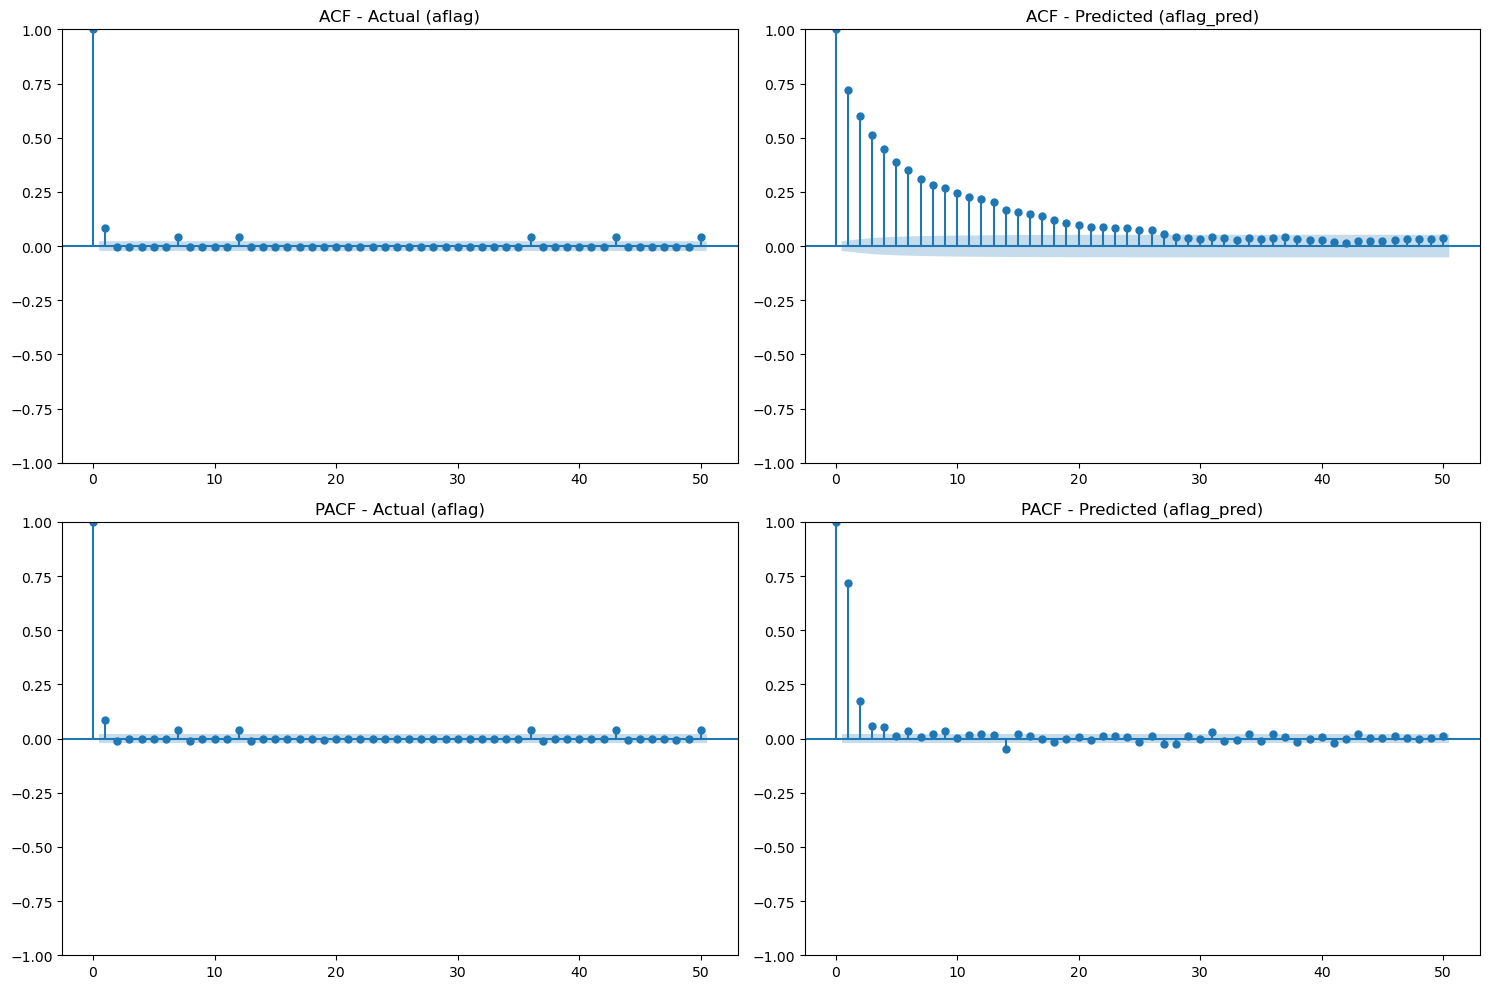
\includegraphics[width=0.95\linewidth]{figures/ACF_181330_benchmark.png}
    \caption{Autocorrelation (ACF) and Partial Autocorrelation (PACF) plots of actual and benchmark predicted aggressive trade series}
    \caption*{\textit{Note:} The plot confirms that the benchmark pattern is very different from both the true and model-predicted series in Figure~\ref{fig:acf-pacf}.}
    \label{fig:acf-pacf-com}
\end{figure}

Table~\ref{tb:ks-test-com} compares the Kolmogorov--Smirnov (KS) test results between the benchmark and the model. The KS statistic for the model is only 0.0019, compared to 0.1054 for the benchmark. This shows that the predicted event time distribution from the model is much closer to the true distribution than the benchmark. The p-value for the model is 1.0000, meaning there is no significant difference between the predicted and actual distributions. 
In contrast, the benchmark's p-value is 0.0000, indicating a clear mismatch.  The predicted proportion of aggressive trades from the model is 0.0049, which is very close to the actual proportion of 0.0030. Meanwhile, the benchmark predicts 10.84\% of events as aggressive, far from the actual value. The proportion difference is only 0.0019 for the model, but 0.1054 for the benchmark. These results show that the model not only matches the number of aggressive trades more accurately but also better captures their overall distribution over time.

\begin{table}[H]
    \centering
    \caption{Kolmogorov--Smirnov Test Results Comparison}
    \caption*{\textit{Note:} The statistical difference between actual and predicted aggressive trade event distributions using the Kolmogorov--Smirnov (KS) test. A smaller KS statistic and a larger p-value indicate better alignment. The model's KS statistic is much lower (0.0019) compared to the benchmark (0.1054), and its p-value is 1.0000, showing no significant difference from the actual data. In contrast, the benchmark has a p-value of 0.0000, meaning its prediction is statistically different from the real distribution. The model also gives a predicted aggressive trade proportion of 0.0049, which is much closer to the actual 0.0030 than the benchmark's 0.1084.}
    \label{tb:ks-test-com}
    \begin{tabular}{lrr}
    \toprule
    Metric & Benchmark Value & Model Value\\
    \midrule
    KS Statistic & 0.1054 & 0.0019 \\
    p-value & 0.0000 & 1.0000 \\
    Significant ($p < 0.05$) & True & False \\
    Actual Proportion & 0.0030 & 0.0030 \\
    Predicted Proportion & 0.1084 & 0.0049 \\
    Proportion Difference & 0.1054 & 0.0019 \\
    \bottomrule
    \end{tabular}
\end{table}

\chapter{Conclusions and Discussion}\label{chapter:cd}
% discussion of the outcomes
In conclusion, the results in Chapter~\ref{chapter:experiments} show that our framework has good alignment with real FX spot market in both the market conditions, temporal dependencies and clustering properties of aggressive trades. By using the XGBoost filter, class imbalance gets solved, and the Neural Hawkes Process is able to fits well with the true pattern of aggressive trade. The model gives realistic and dynamic predictions, which are two critical requirements confirmed by evaluation metrics results. By clear short-term excitation, fast decay, and intensity, the model is capable to be explained clearly why an aggressive trade occurs and why not. It is more robust and transparent than black-box models, and more sophisticated and dynamic than single stochastic model. It is useful for building better and more realistic backtesting environments.

% Comparison with Existing Approache, simplications for FX backtesting environments
Compared to the existing backtesting approach at MN as shown in Table~\ref{tab:filling_spread}, our method gives a more realistic and dynamic view of order filling method. The traditional backtesting method uses filling probabilities based on spread only. This is simple and fast, but it does not reflect how aggressive trades happen in the market, thus loses many transaction opportunities. It ignores the clustering of trades and changes in market conditions. By the use of our model, it captures how often trades happen and when they happen. This makes the backtesting more realistic, dynamic and closer to real market scenarios. 

% Potential applications beyond FX, e.g., equities, crypto markets.
Besides the use in FX spot market, it is also appliable in other high-frequent trading markets, like equities and crypto. Outside the financial field, it can also be used for classification prediction problems with extreme class imbalance, like medical disease detection, fraud detection in banking, network intrusion detection in cybersecurity, and rare event prediction in industrial systems. In all these cases, events are rare, depend on time and conditions, and require models that can capture both sequence and intensity patterns, which our framework is designed to do.

% Future Research Directions and possible improvement
There are also some ways to improve our work in the future. First, the model can be extended to simulate multiple types of market events, not just aggressive trades. This would help build a more complete market environment. Second, the current model focuses on one market. Future work can explore multi-asset or cross-market scenarios to test trading strategies across different markets. Finally, the model now uses fixed features calculated by order book information for prediction. It might help to include more features, such as news sentiment. 


%\makeglossaries
% \newglossaryentry{CBOE}{
%     name={Chicago Board Options Exchange},
%     description={The Chicago Board Options Exchange (CBOE), founded in 1973, is the world's largest options exchange. It focuses on trading standardized options contracts related to individual equities, indexes, and interest rates.}
% }


\newglossaryentry{parallel execution}{
    name={parallel execution},
    description={Parallel execution refers to the process of running multiple tasks or operations simultaneously rather than sequentially. In trading algorithms, it enables multiple child orders to be submitted to different venues at the same time, improving execution speed and optimizing order distribution while maintaining market efficiency.}
}

\newglossaryentry{venues}{
    name={venues},
    description={Venue is exchange in the financial market.}
}

\newacronym{lob}{LOB}{limit order book}

\newglossaryentry{microstructure of financial markets}{
    name={microstructure of financial markets},
    description={Market microstructure is the study of how financial markets work at a detailed level — how trades happen, how prices are set, and how buyers and sellers interact in real time.}
}

\printglossary[type=\acronymtype, title=Acronyms]
\printglossary

%Choose a good bibliography style, plain would do often, but these might be nice too
%\bibliographystyle{these}
\bibliographystyle{plainnat}
\bibliography{references}

\newpage
\appendix
\input{appendices/main}


\end{document}
